% +--------------------------------------------------------------------+
% | Chapter 04 - T-power invariant implications				   |
% +--------------------------------------------------------------------+

\graphicspath{{./_figures/04_tpowerinvariant/}}

\section{Introduction}

From a pragmatic aspect of language, linguistic modifiers are defined as words that can be used to strengthen or weaken the force in which an statement is expressed \cite{Nikula1996}. For instance, it is clear that in natural language words like \textit{unlikely}, \textit{sort of}, \textit{certainly}, \textit{rather}, \textit{very} or \textit{extremely} modify the meaning of an statement. With respect to fuzzy logic, linguistic modifiers (also called ``fuzzy hedges'') were introduced by Lakoff in \cite{Lakoff1973} as ``words whose job is to make things fuzzier or less fuzzy''. More specifically, fuzzy hedges are defined as operators that transform a fuzzy set into another, normally by modifying the shape of the membership function \cite{Zimmermann1991}. Thus, fuzzy hedges modify the meaning of a fuzzy proposition by changing the membership degrees of the underlying fuzzy sets. Depending on whether they strengthen or soften the impact or meaning of an statement, a distinction between stresser or depresser hedges is made:

\begin{quotation}
	This is a \textit{significant} contribution to the field (stresser).
	
	This is a \textit{modest} contribution to the field (depresser).
\end{quotation}

Formally, any increasing function $h:[0,1] \to [0,1]$ with $h(0)=0$, $h(1)=1$ is considered to be a fuzzy hedge, which is a stresser if $h(a)\leq a$ for all $a \in [0,1]$ and a depresser if $h(a) \geq a$ for all $a \in [0,1]$ \cite{Esteva2011}. For instance, widely-used fuzzy hedges are the following unary operations: $h(a)=a^2$ (usually called concentration and often interpreted as the word \textit{very}) and $h(a)= a^{\frac{1}{2}}$ (usually called dilation and often interpreted as the word \textit{little} or \textit{fairly}) \cite{Zimmermann1991}. More generally, in \cite{Baldwin1979,Nafarieh1991} the functions $h(a)=a^r$ with $r \in (0,+\infty)$ were proposed as a family of fuzzy hedges, which are stressers for all $r > 1$ and depressers for all $r < 1$.

Besides, in \cite{Walker2002} the $r$-th powers of a continuous t-norm $T$, denoted by $a_T^{(r)}$, with $r$ any positive real number were defined and studied in detail. From this study we derive that $a^r=a_{\TP}^{(r)}$ for all $a \in [0,1]$ and $r \in(0,+\infty)$. Then, the family of fuzzy hedges announced before can be written as $h(a)=a_{\TP}^{(r)}$ with $r \in (0,+\infty)$. From this new perspective, the family of unary functions $h(a)=a_T^{(r)}$ with $r \in (0,+\infty)$ can be considered as a family of fuzzy hedges for each continuous t-norm $T$, which are also stressers for all $r>1$ and depressers for all $r<1$ (see Figure \ref{fig:fuzzyhedges} for a graphical representation when $T \in \{\TP,\TLK\}$). Not only this generalization provides plenty of families of fuzzy hedges, but also it allows to define fuzzy hedges based on the same t-norm that could be considered as the fuzzy conjunction in a particular application. In our opinion, this family may be a more coherent choice as a family of fuzzy hedges than $h(a)=a^r$ when the product t-norm is not considered.

	\begin{figure}[h]
	\centering
	\begin{subfigure}[t]{0.5\linewidth}\vspace{0pt}
		\centering
		\begin{tikzpicture}
			\draw ($(4,0) + (0,-2pt)$) -- ($(4,0) + (0,2pt)$);
			\node[below] at (4,0) {$1$};
			\draw ($(0,4) + (-2pt,0)$) -- ($(0,4) + (2pt,0)$);
			\node[left] at (0,4) {$1$};
			\node[below right] at (-0.05,0.05) {$0$};
			\draw[scale=4,->] (-0.1, 0) -- (1.1, 0) node[right] {$a$};
			\draw[scale=4,->] (0, -0.1) -- (0, 1.1) node[above] {$h$};
			\draw[scale=4,samples=1000, domain=0:1, smooth, variable=\x, teal] plot ({\x}, {\x^(0.0625)});
			\draw[scale=4,samples=1000, domain=0:1, smooth, variable=\x, teal] plot ({\x}, {\x^(0.125)});
			\draw[scale=4,samples=1000, domain=0:1, smooth, variable=\x, teal] plot ({\x}, {\x^(0.25)});
			\draw[scale=4,samples=100, domain=0:1, smooth, variable=\x, teal] plot ({\x}, {\x^(0.5)});
			\draw[scale=4, domain=0:1, smooth, variable=\x, purple] plot ({\x}, {\x^2});
			\draw[scale=4, domain=0:1, smooth, variable=\x, purple] plot ({\x}, {\x^4});
			\draw[scale=4, domain=0:1, smooth, variable=\x, purple] plot ({\x}, {\x^8});
			\draw[scale=4, domain=0:1, smooth, variable=\x, purple] plot ({\x}, {\x^16});
		\end{tikzpicture}
		\caption{$T=\TP$}	
	\end{subfigure}~
	\begin{subfigure}[t]{0.5\linewidth}\vspace{0pt}
		\centering
		\begin{tikzpicture}
			\draw ($(4,0) + (0,-2pt)$) -- ($(4,0) + (0,2pt)$);
			\node[below] at (4,0) {$1$};
			\draw ($(0,4) + (-2pt,0)$) -- ($(0,4) + (2pt,0)$);
			\node[left] at (0,4) {$1$};
			\node[below right] at (-0.05,0.05) {$0$};
			\draw[scale=4,->] (-0.1, 0) -- (1.1, 0) node[right] {$a$};
			\draw[scale=4,->] (0, -0.1) -- (0, 1.1) node[above] {$h$};
			\draw[scale=4,samples=1000, domain=0:1, smooth, variable=\x, teal] plot ({\x}, {1-0.0625*(1-\x)});
			\draw[scale=4,samples=1000, domain=0:1, smooth, variable=\x, teal] plot ({\x}, {1-0.125*(1-\x)});	
			\draw[scale=4,samples=1000, domain=0:1, smooth, variable=\x, teal] plot ({\x}, {1-0.25*(1-\x)});	
			\draw[scale=4,samples=1000, domain=0:1, smooth, variable=\x, teal] plot ({\x}, {1-0.5*(1-\x)});
			\draw[scale=4,samples=1000, domain=0:1, smooth, variable=\x, purple] plot ({\x}, {(\x<=0.5)*(0)+(\x>0.5)*(1-2*(1-\x))});
			\draw[scale=4,samples=1000, domain=0:1, smooth, variable=\x, purple] plot ({\x}, {(4*\x<=3)*(0)+(4*\x>3)*(1-4*(1-\x))});
			\draw[scale=4,samples=1000, domain=0:1, smooth, variable=\x, purple] plot ({\x}, {(8*\x<=7)*(0)+(8*\x>7)*(1-8*(1-\x))});
			\draw[scale=4,samples=1000, domain=0:1, smooth, variable=\x, purple] plot ({\x}, {(16*\x<=15)*(0)+(16*\x>15)*(1-16*(1-\x))});
		\end{tikzpicture}
		\caption{$T=\TLK$}
	\end{subfigure}
	\caption{Plot of $h(a)=a_T^{(r)}$ for all $r \in \{\frac{1}{16},\frac{1}{8},\frac{1}{4},\frac{1}{2},2,4,8,16\}$ for the cases $T \in \{\TP,\TLK\}$. Stressers are colored in purple and depressers in teal.}\label{fig:fuzzyhedges}
\end{figure}

In \cite{Mizumoto1982}, Mizumoto and Zimmermann presented the following example of fuzzy propositions involving fuzzy hedges:
\begin{quotation}
	If the tomato is red, then it is ripe.
	
	If the tomato is \textit{very} red, then it is \textit{very} ripe.
	
	If the tomato is \textit{little} red, then it is \textit{little} ripe.
\end{quotation}
They studied some properties of several fuzzy reasoning methods in the case of the general Modus Ponens and Modus Tollens applied to this example. An important characteristic of this example is that the antecedent and the corresponding consequent of the fuzzy propositions are affected by the same linguistic modifier (``\textit{very}'', ``\textit{little}''). This fact was considered in \cite{Massanet2017} to propose a novel additional property for fuzzy implication functions called the invariance property. This property relies on the reasonable demand that a fuzzy implication function which is used to model the fuzzy conditionals involved in this problem should provide the same truth value. More generally, the truth value provided by the fuzzy implication function should not change when the same linguistic modifier is applied to the antecedent and the consequent of the fuzzy conditional.


The invariance property was formally defined in \cite{Massanet2017} when the linguistic modifier is modeled through powers of a continuous t-norm. \footnote{The definition of \PIT considered in this chapter corresponds to a slight modification of the original one presented in \cite[Definition~5]{Massanet2017}. We refer the reader to Remark \ref{remark:PITmodification} for the justification of this alteration.}

\begin{definition}
	Let $I$ be a fuzzy implication function and $T$ a continuous t-norm. It is said that $I$ is \emph{invariant with respect to $T$-powers}, or simply that it is $T$-\emph{power invariant} when
	$$
	I(x,y)=I\left(x_T^{(r)}, y_T^{(r)}\right) \eqno {\text{\PIT}}
	$$
	holds for all positive real numbers $r > 0$ and for all $x, y \in (0,1)$ such that $x_T^{(r)}, y_T^{(r)} \not = 0$.
\end{definition}

It is straightforward to check that many of the most usual fuzzy implication functions (\L ukasiewicz, Kleene-Dienes, G\"odel or Yager implications, among others) do not fulfill this property. For that reason, in the same paper, the so-called power based implications were introduced as a family of fuzzy implication functions which fulfill the invariance property with respected to many continuous t-norms (see also the corrigendum \cite{Massanet2019}). Moreover, in \cite{Massanet2019B} the authors characterize all binary functions that are invariant with respect to a certain t-norm $T$, whether it is strict, nilpotent or, more generally, continuous. However, the characterization in the case when $T$ is nilpotent was not entirely correct. Thus, one of the contributions of this chapter is to correct that result and to present the family of fuzzy implication functions characterized by the fact that they are invariant with respect to the positive powers of a strict or nilpotent t-norm, named strict or nilpotent T-power invariant implications, respectively.


 On the other hand, in \cite{Massanet2019B} no other additional properties apart from the invariance were studied and therefore, it is not known whether there exist invariant fuzzy implication functions  satisfying the exchange principle, the left neutrality principle, the law of importation, the generalized modus ponens, or other important additional properties. Since these properties may also be required for a particular problem, it is important to study them jointly with the invariance property. In this chapter, several additional properties of the families of fuzzy implication functions which are invariant with respect to the positive powers of a strict or nilpotent t-norm are deeply analyzed. This study has an important derivation: the characterization of the intersections of this family with ten of the most well-known families of fuzzy implication functions such as $(S,N)$, $R$, $QL$ or Yager's implications, among others. Thus, the operators belonging to these families which satisfy the invariance property with respect to the positive powers of a strict or nilpotent t-norm are characterized. Although one may expect the studies for nilpotent and strict t-norms to be analogous, the two families have quite different properties and the two cases had to be studied separately.


The structure of the chapter is as follows. In Section \ref{section:Tpowerimplications} the families of fuzzy implication functions which are invariant with respect to the positive powers of a strict or nilpotent t-norm, called strict or nilpotent invariant implications, are introduced. In Section \ref{section:additional_propertiesTpower}, several additional properties are studied for these families, determining under which conditions they are fulfilled. From this study, in Section \ref{section:intersectionsTpower}, the intersections of strict and nilpotent $T$-power invariant implications with ten of the most well-known classes are presented. The chapter ends in Section \ref{section:ConclusionsTpowerInvariant} with some conclusions and future work. 

\section{Strict and nilpotent $T$-power invariant implications}\label{section:Tpowerimplications}

In \cite{Massanet2017} (see also \cite{Massanet2019}) the family of $T$-power based implications was introduced as a family of fuzzy implication functions which, for many choices of $T$, fulfills the invariance with respect to linguistic modifiers modeled through powers of continuous t-norms. Moreover, the authors studied other additional properties of these fuzzy implication functions as well as their intersection with the main families of fuzzy implication functions. From this study it was pointed out that $T$-power based implications do not fulfill some of the most common properties of fuzzy implication functions such as \NP or \EP and, as a consequence, they do not belong to the most well-known families of fuzzy implication functions. Recently, a characterization of $T$-power based implications was proposed in \cite{Massanet2019B}. As an intermediate step for solving such characterization, a complete characterization of all binary functions $I:[0,1]^2 \to [0,1]$ which are invariant with respect to $T$-powers where $T$ is a strict, nilpotent and, more generally, continuous t-norm was provided in \cite{Massanet2019B}. Moreover, the authors particularized these solutions to the case when $I$ is a fuzzy implication function. In this section, we recall the respective result in \cite{Massanet2019B} to define the families of strict and nilpotent $T$-power invariant implications, respectively. 

\subsection{Strict $T$-power invariant implications}\label{subsection:strictTpowerimplications}

The next result given in \cite{Massanet2019B} provides the characterization of all binary functions that are invariant with respect to the positive powers of a strict t-norm.
\begin{proposition}[{\bf\cite[Proposition 7]{Massanet2019B}}]\label{prop:strict:charactbintpowerinv}
	Let $T$ be a continuous Archimedean strict t-norm and $t$ an additive generator of $T$. A mapping $I:[0,1]^2 \to [0,1]$ is invariant with respect to $T$-powers if and only if there exists a mapping $\varphi:(0,+\infty) \to [0,1]$ such that $I$ is given by
	$$I(x,y)=\varphi \left(\frac{t(x)}{t(y)}\right), \quad \text{for all } x,y \in (0,1).$$
\end{proposition}
From imposing the conditions of the definition of a fuzzy implication function in the previous proposition, the authors derived the characterization of all fuzzy implication functions that are invariant with respect to the positive powers of a strict t-norm.
\begin{theorem}[{\bf\cite[Theorem 8]{Massanet2019B}}]\label{thm:strict:invimp}
	Let $T$ be a strict t-norm and $t$ an additive generator of $T$. A mapping $I:[0,1]^2 \to [0,1]$ is a fuzzy implication function invariant with respect to $T$-powers if and only if there exists an increasing mapping $\varphi:[0,+\infty] \to [0,1]$ with $\varphi(0)=0$, $\varphi(+\infty)=1$ such that $I$ is given by
	\begin{equation}
		I(x,y)=\varphi \left( \frac{t(x)}{t(y)} \right), \quad \text{for all } (x,y) \in [0,1]^2 \setminus \{(x,0),(1,y) \vert 0<x,y<1\},
		\label{eq:strict:invimpl}
	\end{equation}
	with the convention that $\frac{0}{0}=\frac{+\infty}{+\infty}=+\infty$, and such that the remaining values $I(x,0)$ and $I(1,y)$ preserve the monotonicity conditions.
\end{theorem}

Since our aim is to study the family of fuzzy implication functions described in the theorem above, we first provide a concrete definition of such family analyzing in more depth which properties must fulfill $I(x,0)$ and $I(1,y)$ to guarantee that the monotonicities in the definition of a fuzzy implication function are satisfied.

Let $T$ be a strict t-norm, $t$ an additive generator of $T$ and $I:[0,1]^2 \to [0,1]$ a fuzzy implication function invariant with respect to $T$-powers. According to Theorem \ref{thm:strict:invimp}, there exists an increasing function $\varphi:[0,+\infty] \to [0,1]$ with $\varphi(0)=0$, $\varphi(+\infty)=1$ such that $I$ is given by Equation (\ref{eq:strict:invimpl}). First of all, notice that this representation of $I$ is independent from the choice of the generator $t$, because the additive generator of a t-norm is unique up to a multiplicative constant. Now, let us fix the notation of $f(x)=I(x,0)$ for all $x \in (0,1)$ and $g(y)=I(1,y)$ for all $y \in (0,1)$. According to Theorem \ref{thm:strict:invimp}, $I$ is a fuzzy implication function whenever the monotonicity conditions \Ione and \Itwo are fulfilled with the chosen functions $f$ and $g$. From \Ione we get that $f$ needs to be a decreasing function and from \Itwo we get that $g$ has to be an increasing function. Under such conditions, the next lemma proves that the monotonicities  \Ione and \Itwo are equivalent to a single inequality that involves the functions $f$, $g$ and $\varphi$.
\begin{lemma}\label{lem:strict:monotonicity_condition}
	Let $\varphi:[0,+\infty]\to[0,1]$ be an increasing mapping with $\varphi(0)=0$ and $\varphi(+\infty)=1$, $T$ a strict t-norm and $t$ an additive generator of $T$. Let $I:[0,1]^2\to[0,1]$ be a binary mapping invariant with respect to $T$-powers given by Equation (\ref{eq:strict:invimpl}). Then $I$ is a fuzzy implication function if and only if $f(x)=I(x,0)$ for all $x\in(0,1)$ is decreasing, $g(y)=I(1,y)$ for all $y\in(0,1)$ is increasing and
	\begin{equation}\label{eq:strict:monotonicity_condition}
		\displaystyle\inf_{w \in (0,+\infty)} \varphi (w) \geq \max \left\lbrace \sup_{y \in (0,1)} g(y), \sup_{x \in (0,1)} f(x) \right\rbrace.
	\end{equation}
\end{lemma}
\begin{proof} Let us consider first that $I$ is a fuzzy implication function. Therefore, it satisfies \Ione and \Itwo. Fix an arbitrary $w_0 \in (0,+\infty)$. Let us consider $x_0 \in (0,1)$, then taking $y_0=t^{-1}\left(\frac{t(x_0)}{w_0}\right)$ we have that
	$$\varphi(w_0)=\varphi \left(\frac{t(x_0)}{t(y_0)}\right)=I(x_0,y_0) \geq I(x_0,0) =f(x_0).$$
	Thus, $\varphi(w_0) \geq f(x)$ for all $x \in (0,1)$. On the other hand, consider $y_0 \in (0,1)$, then taking $x_0=t^{-1}(w_0t(y_0))$ we get
	$$\varphi(w_0)=\varphi \left(\frac{t(x_0)}{t(y_0)}\right)=I(x_0,y_0) \geq I(1,y_0) =g(y_0),$$
	and then $\varphi(w_0) \geq g(y)$ for all $y\in(0,1)$. Thus,
	$$\varphi(w_0) \geq \max \left\lbrace \sup_{y \in (0,1)} g(y), \sup_{x \in (0,1)} f(x) \right\rbrace, \quad \text{for all } w_0 \in (0,+\infty).$$
	Clearly, Inequality (\ref{eq:strict:monotonicity_condition})  follows. Conversely, assume that $f(x)=I(x,0)$ is decreasing, $g(y)=I(1,y)$ is increasing  and  $\varphi$, $f$ and $g$ satisfy Inequality (\ref{eq:strict:monotonicity_condition}). Let us consider $x_1 \leq x_2 <1$ and $y \in (0,1]$, then
	$$I(x_1,y)=\varphi\left(\frac{t(x_1)}{t(y)}\right)\geq \varphi\left(\frac{t(x_2)}{t(y)}\right)=I(x_2,y),$$
	$$I(x_2,y)= \varphi \left(\frac{t(x_2)}{t(y)}\right) \geq g(y)=I(1,y),$$
	and $I$ satisfies \Ione. On the other hand, for $0<y_1 \leq y_2$ and $x \in [0,1)$ we have that
	$$I(x,y_1)=\varphi\left(\frac{t(x)}{t(y_1)}\right)\leq \varphi\left(\frac{t(x)}{t(y_2)}\right)=I(x,y_2),$$
	$$ I(x,0) = f(x) \leq \varphi \left(\frac{t(x)}{t(y_1)}\right)=I(x,y_1),$$
	and $I$ satisfies \Itwo. Finally, \Ithree directly follows by Equation (\ref{eq:strict:invimpl}).
\end{proof}
Considering the above, we can explicitly define now the family of strict $T$-power invariant implications as the fuzzy implication functions which are invariant with respect to $T$-powers where $T$ is a strict t-norm.
% Definicio %
\begin{definition}\label{def:strict:TPowerInv} Let $T$ be a strict t-norm and $t$ an additive generator of $T$. Let $f:(0,1) \to [0,1]$ be a decreasing function and $\varphi : [0,+\infty] \to [0,1]$, $g:(0,1) \to [0,1]$  increasing functions such that $ \varphi(0)=0$,  $\varphi(+\infty)=1$ and 
	\begin{equation}
		\displaystyle\inf_{w \in (0,+\infty)} \varphi (w) \geq \max \left\lbrace \sup_{y \in (0,1)} g(y), \sup_{x \in (0,1)} f(x) \right\rbrace.
		\label{eq:strict:TPowerInv:MonotonicityCond}
	\end{equation}
	The function $I^T_{\varphi,f,g}:[0,1]^2 \to [0,1]$ defined by
	\begin{equation}
		I^T_{\varphi,f,g}(x,y) =\left\{ \begin{array}{ll}
			f(x) &   \text{if }   x \in (0,1) \text{ and } y=0, \\
			g(y) &  \text{if }  x = 1 \text{ and } y\in (0,1), \\
			\varphi \left(\frac{t(x)}{t(y)}\right) &  \text{otherwise},
		\end{array}
		\right.
		\label{eq:strict:TPowerInv:Expression}
	\end{equation}
	with the understanding $\frac{0}{0}=\frac{+\infty}{+\infty}=+\infty$, is called a \emph{\STP}.
\end{definition}

\begin{remark} In \cite{Massanet2017} it was proved that,  if $T$ is a strict t-norm, $t$ is an additive generator of $T$ and $I^T$ is the corresponding power based implication which is given by
	$$ 
	I^{T}(x,y) =\left\{ \begin{array}{ll}
		1 &   \text{if }   x \leq y, \\
		\frac{t(x)}{t(y)} &  \text{if } x>y,
	\end{array}
	\right.
	$$
with the convention that $\frac{a}{+\infty}=0$ for all $a \in [0,+\infty)$, then $I^T$ is invariant with respect to $T$-powers. Therefore, $I^T$ is also a \STP. Indeed, by considering $f(x)=g(y)=0$ for all $x,y \in (0,1)$ and
	$$ 
	\varphi(x) =\left\{ \begin{array}{ll}
		x &   \text{if }   x < 1, \\
		1 &  \text{if } x \geq 1,
	\end{array}
	\right.
	$$
	we have that $\IT = I^T$.
\end{remark}

% Exemple 1 %
\begin{example}\label{ex:strict:TPowerInv} Let us show two examples of strict $T$-power invariant implications. While the first one is not a power based implication, the second one belongs to that family.
	\begin{enumerate}[label=(\roman*)]
		\item Let us consider $t(s)=\frac{1-s}{s}$ for all $s \in [0,1]$, $f(x)=\frac{1-x}{3}$ for all $x \in (0,1)$, $g(y)=\frac{y}{3}$ for all $y \in(0,1)$  and
		$$\varphi(w)= \left\{ \begin{array}{ll}
			0 &   \text{if }   w=0, \\
			\frac{w+1}{w+3} &  \text{otherwise}. 	\end{array}
		\right.
		$$
		The corresponding strict $T$-power invariant implication is given by
		\begin{equation*}
			I_1(x,y) =\left\{ \begin{array}{ll}
				1 & \text{if } (x,y) \in \{(1,1),(0,0)\},\\
				\frac{1-x}{3} &   \text{if }   x \in (0,1] \text{ and } y=0, \\
				\frac{y}{3} &  \text{if }  x = 1 \text{ and } y\in (0,1), \\
				\frac{y-2xy+x}{y-4xy+3x} &  \text{otherwise}.
			\end{array}
			\right.
		\end{equation*}
		\item Let us consider $t(s)=\frac{1-s}{s}$ for all $s \in [0,1]$, $f(x)=g(y)=0$ for all $x,y \in (0,1)$ and 
		$$\varphi(w)= \left\{ \begin{array}{ll}
			w &   \text{if }   w < 1, \\
			1 &  \text{otherwise}. 	\end{array}
		\right.
		$$
		The corresponding strict $T$-power invariant implication is given by
		\begin{equation*}
			I_2(x,y) =\left\{ \begin{array}{ll}
				0 &   \text{if }   (x \in (0,1] \text{ and } y=0) \text{ or } (x = 1 \text{ and } y\in (0,1)), \\
				\frac{(1-x)y}{(1-y)x} & \text{if }   0<x<y<1,\\
				1 &  \text{otherwise}.
			\end{array}
			\right.
		\end{equation*}
		These two fuzzy implication functions are displayed in Figure \ref{exfig:strict:TPowerInv}.		
		\begin{figure}
			\centering
			\begin{subfigure}{.5\textwidth}
				\centering
				\includegraphics[width=.6\linewidth]{Ex1.pdf}
				\caption{$I_1$}
				\label{exfig:strict:TPowerInv:subfig1}
			\end{subfigure}%
			\begin{subfigure}{.5\textwidth}
				\centering
				\includegraphics[width=.6\linewidth]{Ex2.pdf}
				\caption{$I_2$}
				\label{exfig:strict:TPowerInv:subfig2}
			\end{subfigure}
			\caption[Plot of two examples of strict $T$-power invariant implications.]{Plots of fuzzy implication functions given in Example \ref{ex:strict:TPowerInv}.}
			\label{exfig:strict:TPowerInv}
		\end{figure}
	\end{enumerate}
\end{example}

\subsection{Nilpotent $T$-power invariant implications}\label{subsection:nilpotentTpowerimplications}

The authors in \cite{Massanet2019B} proposed the following characterization of all binary mappings satisfying the $T$-power invariance with respect to a nilpotent Archimedean t-norm $T$ in terms of an additive generator $t$ such that $t(0)>1$.

\begin{proposition}[{\bf \cite[Proposition~11]{Massanet2019B}}]\label{prop:nilpot:mistake}
	Let $T$ be a nilpotent t-norm and $t$ an additive generator of $T$ with $t(0)>1$. Then a mapping $I:[0,1]^2 \to [0,1]$ is invariant with respect to $T$-powers if and only if there exists a mapping $\varphi:(0,+\infty) \to [0,1]$ such that $I$ is given by
	$$I(x,y)=\varphi \left(\frac{t(x)}{t(y)}\right), \quad \text{for all } x,y \in (0,1) \text{ such that } \frac{t(x)}{t(y)}<t(0).$$
\end{proposition}

However, the next example shows that the result is not entirely correct since it provides necessary but not sufficient conditions.

\begin{example}\label{example:nilpot:counterexample}
	Let us consider the Łukasiewicz t-norm \TLK, the additive generator $t(x)=2(1-x)$ for all $ x \in [0,1]$ with $t(0)=2$ and the following binary function
	\begin{equation*}
		I(x,y) =\left\{ \begin{array}{ll}
			\frac{1}{2} \cdot \frac{1-x}{1-y} & \text{if } \frac{1-x}{1-y}<2,\\
			x &   \text{otherwise}.
		\end{array}
		\right.
	\end{equation*}
	If we define $\varphi:(0,+\infty) \to (0,1)$ with $\varphi(w)=\frac{w}{2}$ for all $w \in (0,+\infty)$ we have $I(x,y)= \frac{1}{2} \cdot \frac{1-x}{1-y} =\varphi \left( \frac{t(x)}{t(y)} \right)$ for all $x,y \in [0,1]$ such that $\frac{1-x}{1-y}<2$. Then, the function $I$ fulfills the conditions in Proposition \ref{prop:nilpot:mistake}. However, let us show that $I$ is not invariant with respect to $T$-powers. Consider $x=r=\frac{1}{2}$ and $y = \frac{7}{8}$, then
	$$ x_T^{(r)} = t^{-1}(\min\{t(0),rt(x)\})= t^{-1}(1-x) = \frac{1}{2}+ \frac{x}{2}=\frac{1}{2} + \frac{1}{4}=\frac{3}{4}, \quad y_T^{(r)} = \frac{1}{2} +\frac{y}{2}=\frac{1}{2} + \frac{7}{16} = \frac{15}{16}.$$ 
	In this case,
	$$I(x,y)=I\left(\frac{1}{2},\frac{7}{8}\right) = \frac{1}{2} \not = \frac{3}{4} = I\left(\frac{3}{4}, \frac{15}{16} \right) = I\left(x_T^{(r)},y_T^{(r)}\right).$$
\end{example}

Therefore, differently from the case of strict T-power invariant implications, before presenting the family of nilpotent $T$-power invariant implications we need to study which binary functions are invariant with respect to the positive powers of a nilpotent t-norm, fixing the previous result. In the next result, we present a new characterization of such functions.

\begin{theorem}\label{thm:nilpot:invimp}
	Let $T$ be a nilpotent t-norm and $t$ an additive generator of $T$. Then a mapping $I:[0,1]^2 \to [0,1]$ is invariant with respect to $T$-powers if and only if there exists a mapping $\varphi:(0,+\infty) \to [0,1]$ such that $I$ is given by
	\begin{equation}\label{eq:nilpot:invimpl}
		I(x,y)=\varphi \left(\frac{t(x)}{t(y)}\right), \quad \text{for all } x,y \in (0,1).
	\end{equation}
\end{theorem}
\begin{proof} Let $T$ be a nilpotent t-norm, $t$ an additive generator of $T$ and $I:[0,1]^2 \to [0,1]$ a binary function.
	\begin{itemize}
		\item[$(\Rightarrow)$] Consider the following partition $\displaystyle (0,+\infty)=(0,2) \cup  \bigcup_{n \in \NN}[2^n,2^{n+1})$. Now, let us define the following family of functions
		$$
		\begin{array}{rcl}
			\varphi_0:\left(0,2\right)&\longrightarrow&[0,1]\\
			z&\longmapsto& I\left(t^{-1}\left(\frac{t(0)}{2}z\right),t^{-1}\left(\frac{t(0)}{2}\right)\right),
		\end{array}
		$$
		$$
		\begin{array}{rcl}
			\varphi_n:\left[2^n,2^{n+1}\right)&\longrightarrow&[0,1]\\
			z&\longmapsto& I\left(t^{-1}\left(\frac{t(0)}{2^{n+1}}z\right),t^{-1}\left(\frac{t(0)}{2^{n+1}}\right)\right)
		\end{array},
		\quad
		\text{for all } n \in \NN.
		$$
		These functions are well defined because $\frac{t(0)}{2^{n+1}} \in (0,t(0))$ and
		$$\frac{t(0)}{2^{n+1}}z \in \left[\frac{t(0)}{2^{n+1}} \cdot 2^n ,\frac{t(0)}{2^{n+1}} \cdot 2^{n+1}\right) = \left[\frac{t(0)}{2},t(0)\right) \subseteq (0,t(0)),$$
		for all $n \in \NN$ and $z \in [2^n,2^{n+1})$. Consider the function $\varphi$ defined as follows
		$$
		\begin{array}{rcll	}
			\varphi:(0,+\infty)&\longrightarrow&[0,1]\\
			z&\longmapsto& \varphi_n(z) &\text{if } z \in [2^n,2^{n+1})\\
			z&\longmapsto& \varphi_0(z) &\text{if } z \in (0,2)
		\end{array}.
		$$
		Let us see that $I(x,y)= \varphi \left(\frac{t(x)}{t(y)}\right)$ for all $x,y \in (0,1)$. Since $I$ is $T$-power invariant, then
		$$I(x,y)= I(t^{-1}(rt(x)),t^{-1}(rt(y))),$$
		for all $x,y \in (0,1)$ and $r < \min \left\lbrace\frac{t(0)}{t(x)},\frac{t(0)}{t(y)}\right\rbrace$. Let $x_0,y_0 \in (0,1)$, we distinguish between two cases:
		\begin{itemize}
			\item If $\frac{t(x_0)}{t(y_0)} \in \left[2^n,2^{n+1}\right)$ for some $n \in \NN$, considering $r_0= \frac{t(0)}{2^{n+1}t(y_0)}$ we have that
			$$\frac{t(x_0)}{t(y_0)}< 2^{n+1} \Rightarrow \frac{t(0)}{t(x_0)} > \frac{t(0)}{2^{n+1}t(y_0)} =r_0 \Rightarrow r_0 < \min \left\lbrace\frac{t(0)}{t(x_0)},\frac{t(0)}{t(y_0)}\right\rbrace.$$
			Therefore, 
			\begin{eqnarray*}
				I(x_0,y_0)&=&I(t^{-1}(r_0t(x_0)),t^{-1}(r_0t(y_0)))=I\left(t^{-1}\left(\frac{t(0)}{2^{n+1}}\frac{t(x_0)}{t(y_0)}\right),t^{-1}\left(\frac{t(0)}{2^{n+1}}\right)\right) \\
				&=&\varphi_n\left(\frac{t(x_0)}{t(y_0)}\right) = \varphi \left(\frac{t(x_0)}{t(y_0)}\right).
			\end{eqnarray*}
			\item If $\frac{t(x_0)}{t(y_0)} \in \left(0,2\right)$ then considering $r_0= \frac{t(0)}{2t(y_0)}$ and with an analogous argument to the previous point we obtain that $I(x_0,y_0)=\varphi_0\left(\frac{t(x_0)}{t(y_0)}\right)=\varphi\left(\frac{t(x_0)}{t(y_0)}\right)$.
		\end{itemize}
		\item[$(\Leftarrow)$] Consider that there exists a function $\varphi:(0,+\infty) \to [0,1]$ such that $I$ is given by Equation (\ref{eq:nilpot:invimpl}). We have to prove that $I(x_T^{(r)},y_T^{(r)})=I(x,y)$ for all $r>0$ and $x,y \in [0,1]$ such that $x_T^{(r)},y_T^{(r)} \not \in \{0,1\}$. Since $T$ is a nilpotent t-norm we have that whenever $x_T^{(r)} \not = 0$ then $x_T^{(r)}=t^{-1}(rt(x))$. In this case, we have that
		$$I(x_T^{(r)},y_T^{(r)})=\varphi \left(\frac{t(x_T^{(r)})}{t(y_T^{(r)})}\right)
		=\varphi \left(\frac{rt(x)}{rt(y)}\right) =\varphi \left(\frac{t(x)}{t(y)}\right)=I(x,y).$$
	\end{itemize}
\end{proof}

This result reveals that the structure of functions which are $T$-power invariant is the same in the strict and nilpotent cases (see Proposition \ref{prop:strict:charactbintpowerinv}). Moreover, differently from Proposition \ref{prop:nilpot:mistake}, Equation (\ref{eq:nilpot:invimpl}) is also valid for additive generators with $t(0) \leq 1$. In consequence of this dependence, in \cite{Massanet2019B} the authors only studied fuzzy implication functions which are invariant with respect to the positive powers of a nilpotent t-norm and also satisfy \IP. In our case, thanks to the previous result we can easily characterize all the fuzzy implication functions that are invariant with respect to the positive powers of a nilpotent t-norm without further restrictions.

It is well known that the additive generators of nilpotent t-norms differ from those from strict t-norms in the fact that their image is $[0,t(0)]$ with $t(0)<+\infty$. We will see along the chapter that this fact makes a huge difference between the strict and nilpotent cases. The next trivial lemma will be useful throughout the chapter to the manipulation of Equation  (\ref{eq:nilpot:invimpl}) in the nilpotent case.
\begin{lemma}\label{lem:nilpot:values} 
	Let $w_1,w_2 \in (0,+\infty)$ with $w_1 \leq w_2$ and $t$ an additive generator of a nilpotent t-norm. Then there exist $y^*,x_1,x_2 \in (0,1)$ with $x_1 \geq x_2$ such that $w_1=\frac{t(x_1)}{t(y^*)}$ and $w_2=\frac{t(x_2)}{t(y^*)}$.
\end{lemma}
\begin{proof}
	Since $t$ is a continuous, strictly decreasing function then $\left\lbrace \frac{t(0)}{t(y)} \bigm| y \in (0,1)\right\rbrace = (1,+\infty)$ and there exists a $y^* \in (0,1)$ such that $w_1,w_2 \in \left(0,\frac{t(0)}{t(y^*)}\right)$. On the other hand, we have that $\left\lbrace \frac{t(x)}{t(y^*)} \bigm| x \in (0,1)\right\rbrace = \left(0,\frac{t(0)}{t(y^*)}\right)$ and then there exist $x_1,x_2 \in (0,1)$ such that $w_1=\frac{t(x_1)}{t(y^*)}$ and $w_2=\frac{t(x_2)}{t(y^*)}$. Since $t$ is a strictly decreasing function and $w_1 \leq w_2$ we know that $x_1 \geq x_2$.
\end{proof}

The next result restricts Theorem \ref{thm:nilpot:invimp} to fuzzy implication functions.

\begin{proposition}\label{prop:nilpot:TPowerInv}
	Let $T$ be a nilpotent t-norm and $t$ an additive generator of $T$. A mapping $I:[0,1]^2 \to [0,1]$ is a fuzzy implication function invariant with respect to $T$-powers if and only if $f(x)=I(x,0)$ for all $x \in (0,1)$ is decreasing, $g(y)=I(1,y)$ for all $y \in (0,1)$ is increasing and there exists an increasing function $\varphi:[0,+\infty] \to [0,1]$ such that $\varphi(0)=0$, $\varphi(+\infty)=1$, 
	\begin{equation}\label{eq:prop:nilpot:TPowerInv:MonotonicityCond}
		f(x) \leq \inf_{y \in (0,1)} \varphi \left(\frac{t(x)}{t(y)}\right), \quad \text{for all } x \in (0,1), \quad
		g(y) \leq \inf_{x \in (0,1)} \varphi \left(\frac{t(x)}{t(y)}\right), \quad \text{for all } y \in (0,1),
	\end{equation}
	and $I$ is given by
	\begin{equation}\label{eq:prop:nilpot:TPowerInv:Expression}
		I(x,y) =\left\{ \begin{array}{ll}
			1 & \text{if } x=0 \text{ and } y \in [0,1),\\
			f(x) &   \text{if }   x \in (0,1) \text{ and } y=0, \\
			g(y) &  \text{if }  x = 1 \text{ and } y\in (0,1), \\
			\varphi \left(\frac{t(x)}{t(y)}\right) &  \text{otherwise},
		\end{array}
		\right.
	\end{equation}
	with the understanding $\frac{0}{0} = +\infty$.
\end{proposition}
\begin{proof}
	Let $I$ be a fuzzy implication function which is invariant with respect to $T$-powers. By Theorem \ref{thm:nilpot:invimp} 
	we know that there exists a function $\varphi:(0,+\infty) \to [0,1]$ such that
	$$I(x,y)=\varphi \left(\frac{t(x)}{t(y)}\right), \quad \text{for all }x,y \in (0,1).$$
	We extend this function to $[0,+\infty]$ by defining $\varphi(0)=0$ and $\varphi(+\infty)=1$. Let us define $f(x)=I(x,0)$ for all $x \in (0,1)$ and $g(y)=I(1,y)$ for all $y \in (0,1)$. It is clear that by \Ione, $f$ is decreasing and by \Itwo $g$ is increasing. Now, we prove that $\varphi$ is increasing. Consider $w_1,w_2 \in (0,+\infty)$ with $w_1 \leq w_2$. By Lemma \ref{lem:nilpot:values} we know that there exist $x_1,x_2,y^* \in (0,1)$ with $x_1 \geq x_2$ such that $w_1=\frac{t(x_1)}{t(y^*)}$ and $w_2=\frac{t(x_2)}{t(y^*)}$. Now, by \Ione we have
	$$\varphi(w_1) = \varphi \left(\frac{t(x_1)}{t(y^*)}\right) = I(x_1,y^*) \leq I(x_2,y^*) = \varphi \left(\frac{t(x_2)}{t(y^*)}\right) = \varphi(w_2),$$
	and $\varphi$ is increasing. Then, $I$ has the structure in Equation (\ref{eq:prop:nilpot:TPowerInv:Expression}). Consider $\tilde{x},\tilde{y} \in (0,1)$, then by \Ione and \Itwo we have
	$$f(\tilde{x}) = I(\tilde{x},0) \leq I(\tilde{x},y) = \varphi \left( \frac{t(\tilde{x})}{t(y)} \right), \quad \text{for all } y \in (0,1),$$
	$$g(\tilde{y})=I(1,\tilde{y}) \leq I(x,\tilde{y})= \varphi\left(\frac{t(x)}{t(\tilde{y})}\right), \quad \text{for all } x \in (0,1).$$
	Then, $I$ fulfills Condition (\ref{eq:prop:nilpot:TPowerInv:MonotonicityCond}). For the reverse implication, assume that there exist a decreasing function $f:(0,1) \to [0,1]$ and increasing functions $\varphi:[0,+\infty] \to [0,1]$, $g:(0,1) \to [0,1]$ such that $\varphi(0)=0$, $\varphi(+\infty)=1$ and fulfill Condition (\ref{eq:prop:nilpot:TPowerInv:MonotonicityCond}). Let us see that $I$ given by Equation (\ref{eq:prop:nilpot:TPowerInv:Expression}) is a fuzzy implication function.
	\begin{itemize}
		\item Let $x_1,x_2,y \in [0,1]$ with $x_1 < x_2$, then we distinguish between three cases:
		\begin{itemize}
			\item If $y=0$ then since $f$ is decreasing we have $I(x,0)=f(x_1) \geq f(x_2)=I(x_2,0).$
			\item If $y=1$ then $I(x_1,1)=I(x_2,1)=1$.
			\item  If $ y \in (0,1)$ we have
			\begin{itemize}
				\item If $x_1=0$ then $I(x_1,y)=I(0,y)=1 \geq I(x_2,y).$
				\item If $x_1,x_2 \in (0,1)$ then $I(x_1,y)=\varphi \left(\frac{t(x_1)}{t(y)}\right) \geq \varphi \left(\frac{t(x_2)}{t(y)}\right) = I(x_2,y).$
				\item If $x_1 \in (0,1)$ and $x_2=1$ then $I(x_1,y)=\varphi \left(\frac{t(x_1)}{t(y)}\right) \geq g(y)=I(1,y)=I(x_2,y).$
			\end{itemize}
		\end{itemize} 
		Therefore, $I$ fulfills \Ione.
		\item Analogously to the previous point we verify that $I$ fulfills \Itwo.
		\item Since
		$$ I(1,1)= \PHI{1}{1} = \varphi\left(\frac{0}{0}\right)= \varphi(+\infty)=1, \quad I(0,0)=1,$$
		$$I(1,0)=\PHI{1}{0}=\varphi(0)=0,$$
		we have that $I$ satisfies \Ithree. \qedhere
	\end{itemize}
\end{proof}

Now, in view of the last result, we can define the family of fuzzy implication functions characterized by the fact that they are $T$-power invariant with respect to a certain nilpotent t-norm.

\begin{definition}\label{def:nilpot:TPowerInv}
	Let $T$ be a nilpotent t-norm and $t$ an additive generator of $T$. Let $f:(0,1) \to [0,1]$ be a decreasing function and $\varphi:[0,+\infty] \to [0,1]$, $g: (0,1) \to [0,1]$ increasing functions such that $\varphi(0)=0$, $\varphi(+\infty)=1$ and
	\begin{equation}\label{eq:def:nilpot:TPowerInv:MonotonicityCond}
		f(x) \leq \inf_{y \in (0,1)} \varphi \left(\frac{t(x)}{t(y)}\right), \quad \text{for all } x \in (0,1), \quad
		g(y) \leq \inf_{x \in (0,1)} \varphi \left(\frac{t(x)}{t(y)}\right), \quad \text{for all } y \in (0,1).
	\end{equation}
	The function $\IT:[0,1]^2 \to [0,1]$ defined  by
	\begin{equation}\label{eq:nilpot:TPowerInv:Expression}
		I^T_{\varphi,f,g}(x,y) =\left\{ \begin{array}{ll}
			1 & \text{if } x=0 \text{ and } y \in [0,1),\\
			f(x) &   \text{if }   x \in (0,1) \text{ and } y=0, \\
			g(y) &  \text{if }  x = 1 \text{ and } y\in (0,1), \\
			\varphi \left(\frac{t(x)}{t(y)}\right) &  \text{otherwise},
		\end{array}
		\right.
	\end{equation}
	with the understanding $\frac{0}{0} = + \infty$, is called a \emph{nilpotent $T$-power invariant implication}.
\end{definition}

In view of Definitions \ref{def:strict:TPowerInv} and \ref{def:nilpot:TPowerInv}, we can notice that the structure of strict and nilpotent $T$-power invariant implications is very similar (see Figure \ref{fig:TPowerInv}). However, despite this fact we show further in this chapter that both families behave differently.
% Figure 1 %
\begin{figure}[H]
		\centering
		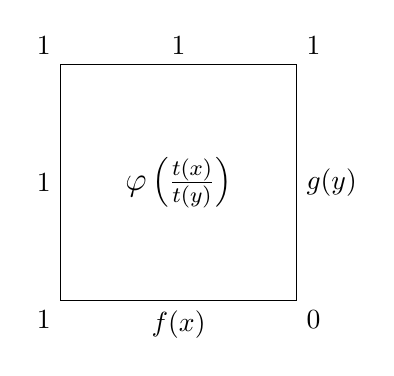
\begin{tikzpicture}[xscale=3, yscale=3]
				\draw (0,0) rectangle (1,1);
				\node [above right] at (1,1) {1} ;
				\node [below right] at (1,0) {0};
				\node [below left] at (0,0) {1};
				\node [above left] at (0,1) {1};
				\node [above] at (0.5,1) {1};
				\node [below] at (0.5,0) {$f(x)$};
				\node [left] at (0,0.5) {1};
				\node [right] at (1,0.5) {$g(y)$};
				\node at (0.5,0.5) {\large $\varphi \left( \frac{t(x)}{t(y)} \right)$};
			\end{tikzpicture}
		\caption{Schema of the structure of the family of strict and nilpotent $T$-power invariant implications.}
		\label{fig:TPowerInv}
\end{figure}

A first difference between Definition \ref{def:nilpot:TPowerInv} and the analogous definition for strict t-norms (see Definition \ref{def:strict:TPowerInv}) is that Condition (\ref{eq:def:nilpot:TPowerInv:MonotonicityCond}) is more complex than Condition (\ref{eq:strict:TPowerInv:MonotonicityCond}). In this case, if $I$ is a fuzzy implication function invariant with respect to $T$-powers where $T$ is a nilpotent t-norm, then  the function $\varphi$ is not necessarily bounded below by any possible value of $f$. For instance, the following example corresponds to a nilpotent $T$-power invariant implication with $\Ima \varphi = [0,1]$ and $f(x)=1-x$ for all $x \in (0,1)$.

\begin{example}\label{ex:nilpot:TPowerInv}
	Let us consider the Łukasiewicz t-norm \TLK, the additive generator $t(x)=1-x$ for all $x \in [0,1]$, $\varphi(w)=w$ for all $w \in [0,1]$, $\varphi(w)=1$ for all $ w \in (1,+\infty]$, $f(x)=1-x$ for all $x \in (0,1)$ and $g(y)=0$ for all $ y \in (0,1)$. We have that $\varphi$, $f$ and $g$ fulfill Condition (\ref{eq:def:nilpot:TPowerInv:MonotonicityCond}) and then the function given by
	$$
	I(x,y) =\left\{ \begin{array}{ll}
		1-x &   \text{if }   x \in (0,1) \text{ and } y=0, \\
		0 &  \text{if }  x = 1 \text{ and } y\in [0,1), \\
		\frac{1-x}{1-y} &  \text{if } x,y \in (0,1) \text{ and } x \geq y, \\
		1 & \text{otherwise,}
	\end{array}
	\right.
	$$
	is a fuzzy implication function which is invariant with respect to the positive powers of \TLK. The plot of this fuzzy implication function is displayed in Figure \ref{exfig:nilpot:TPowerInv}.
	\begin{figure}[!htp]
		\centering
		\includegraphics[scale=0.5]{Example0.pdf}
		\caption[Plot of an example of a nilpotent $T$-power invariant implication.]{Plot of the fuzzy implication function constructed in Example \ref{ex:nilpot:TPowerInv}.}\label{exfig:nilpot:TPowerInv}
	\end{figure}
\end{example}

However, we can simplify Condition (\ref{eq:def:nilpot:TPowerInv:MonotonicityCond}) in terms of the following necessary condition.
\begin{lemma}\label{lem:nilpot:monotonicity_condition:necessicity}
	Let \IT be a nilpotent $T$-power invariant implication, then
	\begin{equation*}
		\sup_{x \in (0,1)} f(x) \leq \inf_{w \in (1,+\infty)} \varphi(w), \quad \sup_{y \in (0,1)} g(y) \leq \inf_{w \in (0,+\infty)} \varphi(w).
	\end{equation*}
\end{lemma}
\begin{proof}
	Let us consider $\tilde{x} \in (0,1)$ and $w_0 \in (1,+\infty)$,  since $t$ is a continuous, strictly decreasing function then $\left\lbrace \frac{t(\tilde{x})}{t(y)} \bigm| y \in (0,1) \right\rbrace = \left(\frac{t(\tilde{x})}{t(0)},+\infty\right)$ with $\frac{t(\tilde{x})}{t(0)}<1$ and $ w_0 \in (1,+\infty)\subseteq \left (\frac{t(\tilde{x})}{t(0)},+\infty\right )$. Thus, there exists a $y_0 \in (0,1)$ with $w_0 = \frac{t(\tilde{x})}{t(y_0)}$ and by \Itwo we have
	$$f(\tilde{x}) = I(\tilde{x},0) \leq I(\tilde{x},y_0) = \PHI{\tilde{x}}{y_0}=\varphi(w_0).$$
	On the other hand, we consider $\tilde{y} \in (0,1)$ and $w_1 \in (0,+\infty)$ and we prove that $g(\tilde{y}) \leq \varphi(w_1)$. Since $\varphi$ is increasing it is enough to consider $w_1 \in (0,1)$. We know that $\left\lbrace \frac{t(x)}{t(\tilde{y})} \bigm| x \in (0,1)\right\rbrace = \left(0,\frac{t(0)}{t(\tilde{y})}\right)$ with $\frac{t(0)}{t(\tilde{y})}>1$ and then $w_1 \in (0,1)\subseteq \left(0,\frac{t(0)}{t(\tilde{y})}\right)$. Thus, there exists an $x_1 \in (0,1)$ with $\frac{t(x_1)}{t(\tilde{y})}=w_1$ and  by \Ione we have
	$$g(\tilde{y})=I(1,\tilde{y}) \leq I(x_1,\tilde{y})=\varphi\left(\frac{t(x_1)}{t(\tilde{y})}\right) =\varphi(w_1).$$
\end{proof}

The following example shows that Lemma \ref{lem:nilpot:monotonicity_condition:necessicity} is not sufficient.

\begin{example}
	Let us consider the Łukasiewicz t-norm \TLK, the additive generator $t(x)=1-x$ for all $x \in [0,1]$, $\varphi(w)=w$ for all $w \in [0,1]$, $\varphi(w)=1$ for all $w \in (1,+\infty]$, $f(x)=1-x^2$ for all $x \in (0,1)$ and $g(y)=0$ for all $ y \in (0,1)$. Let $I$ be the function given by Equation (\ref{eq:nilpot:TPowerInv:Expression}). For $x=\frac{1}{2}$ and $y=\frac{1}{4}$ we have
	$$f\left( \frac{1}{2} \right) = \frac{3}{4} > \frac{2}{3} = I\left(\frac{1}{2},\frac{1}{4}\right),$$
	and since $I$ does not fulfill Condition (\ref{eq:def:nilpot:TPowerInv:MonotonicityCond}), $I$ is not a nilpotent \TLK-power invariant implication. However, we have
	$$\sup_{x \in (0,1)} f(x) = 1= \inf_{w \in (1,+\infty)} \varphi(w), \quad \sup_{y \in (0,1)} g(y)=0 = \inf_{w \in (0,+\infty)} \varphi(w).$$
\end{example}

\begin{remark}
	Let $T$ be a nilpotent (resp. strict) t-norm, when we consider a nilpotent (resp. strict) $T$-power invariant implication $\IT$ we are always assuming that there exist functions $\varphi$, $g$ and $f$ that fulfill all the conditions in Definition \ref{def:nilpot:TPowerInv} (resp. Definition \ref{def:strict:TPowerInv}) even when not explicitly mentioned. For instance, if we say ``Let us consider \IT a nilpotent $T$-power invariant implication with $f(x)\geq 0.5$ for all $x \in (0,1)$'', then $f:(0,1) \to [0,1]$ must be a decreasing function with $0.5 \leq f(x) \leq \inf_{y \in (0,1)} \varphi \left(\frac{t(x)}{t(y)}\right)$ for all $x \in (0,1)$, whenever this is allowed by the structure of $\varphi$.
\end{remark}

\section{Additional properties of strict and nilpotent $T$-power invariant implications}\label{section:additional_propertiesTpower}

In this section, we study other additional properties aside from the invariance with respect to $T$-powers that can be satisfied by the family of strict and nilpotent $T$-power implications. The additional properties we have decided to study are: continuity, natural negation, trivial 1-region, \CB, \NP, \IP, \OP, \EP, \LI, \IB and \TC. We have chosen these properties because they are among the most popular additional properties of fuzzy implication functions. Also, the study of these properties (specially \NP and \EP) is essential for the determination of the intersection between these families and others (see Section \ref{section:intersectionsTpower}). Due to several differences, we perform a separate study for strict and nilpotent $T$-power implications.

\subsection{Additional properties of strict $T$-power invariant implications}\label{subsection:additional_propertiesStrictTpower}

First of all, we establish under which conditions on $\varphi$, $f$ and $g$, the corresponding \STP is continuous on a point of its domain.
% Continuity %
\begin{proposition} \label{prop:strict:continuity} Let $\IT$ be a \STP. The following statements hold:
	\begin{enumerate}[label=(\roman*)]
		\item If $\varphi$ is continuous on $w=0$, then $f(x)=g(y)=0$ for all $x,y \in (0,1)$.
		\item If $\displaystyle \lim_{x \to 0^+} f(x)=1$ or $\displaystyle \lim_{y \to 1^-}g(y)=1$, then $\varphi(w)=1$ for all $w \in (0,+\infty)$.
		\item $\IT$ is continuous on $(x,0)$ for $x \in (0,1)$ if and only if $\displaystyle f(x)= \lim_{w \to 0^+} \varphi(w)$.
		\item $\IT$ is continuous on $(1,y)$ for $y \in (0,1)$ if and only if $\displaystyle g(y)= \lim_{w \to 0^+} \varphi(w)$.
		\item $\IT$ is continuous on $(x,1)$ and $(0,x)$ for all $x \in [0,1]$ if and only if $\displaystyle \lim_{w \to +\infty} \varphi(w)=1$.
		\item $\IT$ is continuous on $(x_0,y_0)$ with $x_0,y_0 \in (0,1)$ if and only if $\varphi$ is continuous on $\frac{t(x_0)}{t(y_0)}$. In this case, $\IT$ is also continuous on the following points
		$$\left(x,t^{-1}\left(\frac{t(x)t(y_0)}{t(x_0)}\right)\right), \quad \text{for all } x \in (0,1).$$
	\end{enumerate}
\end{proposition}
\begin{proof}Statements (i) and (ii) are direct consequences of Condition (\ref{eq:strict:TPowerInv:MonotonicityCond}).
	\begin{enumerate}[label=(\roman*)]
		\item[(iii)] $\IT$ is continuous on $(x_0,0)$ for $x_0 \in (0,1)$ if and only if
		$$f(x_0)=\IT(x_0,0)=\lim_{(x,y) \to (x_0,0)}\IT(x,y) = \lim_{(x,y) \to (x_0,0)} \varphi\left(\frac{t(x)}{t(y)}\right).$$
		Now, by considering the change of variables $w=\frac{t(x)}{t(y)}$ we obtain
		$$\lim_{(x,y) \to (x_0,0)} \varphi\left(\frac{t(x)}{t(y)}\right)=\lim_{w \to 0^+} \varphi(w).$$
		\item[(iv)] The proof is analogous to the Case (iii).
		\item[(v)] $\IT$ is continuous on $(x_0,1)$ for $x_0 \in[0,1]$ if and only if
		$$1=I(x_0,1)=\lim_{(x,y) \to (x_0,1)}I(x,y)=\lim_{(x,y) \to (x_0,1)}\varphi\left(\frac{t(x)}{t(y)}\right)=\lim_{w \to +\infty}\varphi(w).$$ 
		On the other hand, $\IT$ is continuous $(0,x_0)$ for $x_0 \in[0,1]$ if and only if
		$$1=\IT(0,x_0)=\lim_{(x,y) \to (0,x_0)}I(x,y)=\lim_{(x,y) \to (0,x_0)}\varphi\left(\frac{t(x)}{t(y)}\right)=\lim_{w \to +\infty}\varphi(w).$$
		\item[(vi)] $\IT$ is continuous on $(x_0,y_0)$ for $x_0,y_0 \in (0,1)$ if and only if
		$$I(x_0,y_0)=\lim_{(x,y) \to (x_0,y_0)} I(x,y)=\lim_{(x,y) \to (x_0,y_0)} \varphi \left(\frac{t(x)}{t(y)}\right) = \lim_{w \to \frac{t(x_0)}{t(y_0)}}\varphi(w).$$
		Now, since the points $(a_x,b_x)=\left(x,t^{-1}\left(\frac{t(x)t(y_0)}{t(x_0)}\right)\right)$ are such that $\frac{t(a_x)}{t(b_x)}=\frac{t(x_0)}{t(y_0)}$ for all $x \in (0,1)$, we have that $\IT$ is also continuous on $(a_x,b_x)$. \qedhere
	\end{enumerate}
\end{proof}
Notice that the previous proposition implies that imposing continuity in certain points of a \STP leads to consider that $\varphi$, $f$ or $g$ are constant. This is due to Condition (\ref{eq:strict:TPowerInv:MonotonicityCond}), which imposes that the function $\varphi$ is bounded below by any possible value of $f$ and $g$ (see Example \ref{ex:strict:TPowerInv}). Then, although the structure of strict $T$-power implications may seem flexible since it depends on three unknown functions, as a matter of fact, Condition (\ref{eq:strict:TPowerInv:MonotonicityCond}) severely restricts the choices of functions $\varphi$, $f$ and $g$ for which \IT is a fuzzy implication function. Moreover, from (ii)-Proposition \ref{prop:strict:continuity} it is easy to see that \IT is never a continuous function.

\begin{corollary}\label{cor:strict:discontinuous} Let \IT be a \STP. Then at least one of the following conditions holds:
	\begin{enumerate}[label=(\roman*)]
		\item $\IT$ is discontinuous on (1,0).
		\item $\IT$ is discontinuous on (0,0) or (1,1).
	\end{enumerate}
\end{corollary}
\begin{proof} Let us consider \IT a \STP. If \IT is continuous on $(0,0)$ then
	$$ 1=\IT(0,0)= \lim_{x \to 0^+} \IT(x,0) = \lim_{x \to 0^+} f(x), $$
	and by {(ii)-Proposition \ref{prop:strict:continuity}} we get that $\varphi(w)=1$ for all $w \in (0,+\infty)$. Therefore, $\IT(x,y)=1$ for all $(x,y) \in (0,1)^2$. Since $I^T_{\varphi,f,g}(1,0)=0$, $I^T_{\varphi,f,g}$ is discontinuous on $(1,0)$.
	On the other hand, if \IT is continuous on $(1,1)$ then
	$$1=\IT(1,1)= \lim_{y \to 1^-} \IT(1,y) = \lim_{y \to 1^-} g(y), $$
	and again by {(ii)-Proposition \ref{prop:strict:continuity}} we have that $\IT(x,y)=1$ for all $(x,y) \in (0,1)^2$ and then \IT is not continuous on $(1,0)$.
\end{proof}
In terms of the natural negation of a \STP, it is straightforward to see that it is completely determined by the function $f$. Therefore, we can always find strict $T$-power implications  whose natural negation is a certain fuzzy negation $N$. However, again by {(ii)-Proposition \ref{prop:strict:continuity}} we remark that if the natural negation of $\IT$ is continuous on $x=0$ necessarily $\IT$ is constant to 1 in $(0,1)^2$.

% Natural Negation %
\begin{corollary}\label{cor:strict:natural_negation} Let \IT be a \STP. The natural negation of $\IT$ is given by
	$$ N_{\IT}(x)=\left\{ \begin{array}{ll}
		1 &  \text{if }  x=0, \\
		f(x) & \text{if }  x \in(0,1),\\
		0 &  \text{if }x=1.
	\end{array}
	\right.
	$$
	Moreover, if $N_{\IT}$ is continuous on $x=0$ (in particular, when $N_{\IT}$ is a strong or strict negation), then $\IT(x,y)=1$ for all $x,y \in (0,1)^2$.
\end{corollary}
\begin{proof} 
	Let us consider \IT a \STP, then by definition we have that
	$$
	N_{\IT}(x)=\IT(x,0)= \left\{ \begin{array}{ll}
		1 &  \text{if }  x=0, \\
		f(x) & \text{if }  x \in(0,1),\\
		0 &  \text{if }x=1.
	\end{array}
	\right.
	$$
	Now, if it is continuous on $x=0$ then $\displaystyle 1=\lim_{x \to 0^+} N_{\IT}(x) = \lim_{x \to 0^+} f(x)$ and by {(ii)-Proposition \ref{prop:strict:continuity}} we have that $\varphi(w)=1$ for all $w \in (0,+\infty)$. Therefore, $\IT(x,y)=1$ for all $x,y \in (0,1)$.
\end{proof}
% 1-region %
With respect to the 1 and 0-region of a \STP, it is straightforward to see that the region where \IT equals 0 or 1 directly depends on the intervals where the functions $\varphi$, $f$ and $g$ equal 0 or 1, respectively (see Examples \ref{ex:strict:TPowerInv} and \ref{example:strict:(IB)}). However, the next proposition characterizes when $I$ has a trivial 1-region.

\begin{proposition}\label{prop:strict:1-region}
	 Let \IT be a \STP. Then $(I(x,y)=1 \Leftrightarrow x=0 \text{ or } y=1)$ if and only if $f(x),g(y)<1$ for all $x,y \in (0,1)$ and $\varphi(w)<1$ for all $w \in (0,+\infty)$.
\end{proposition} 
\begin{proof} Straightforward from Definition \ref{def:strict:TPowerInv}.
\end{proof}

% Consequent boundary %
The following result studies when strict $T$-power invariant implications satisfy the consequent boundary. In this case, we see that $\IT$ needs to be constant to 1 in $(0,1)^2$ and $g(y) \geq y$ for all $y \in (0,1)$.
\begin{proposition}\label{prop:strict:(CB)} Let $\IT$ be a strict $T$-power invariant implication. Then $\IT$ satisfies \CB if and only if $g(y) \geq y$ for all $y \in (0,1)$. Moreover, in this case \IT is given by
	\begin{equation}\label{eq:(CB)}
		\IT(x,y) = \left\{ \begin{array}{ll}
			0 &  \text{if }  x=1 \text{ and } y=0, \\
			f(x) & \text{if }  x \in(0,1) \text{ and }  y=0,\\
			g(y) &  \text{if }x=1 \text{ and } y \in (0,1), \\
			1 & \text{otherwise.}
		\end{array}
		\right.
	\end{equation}
\end{proposition}
\begin{proof} 
	Assume that $g(y) \geq y$ for all $y \in (0,1)$, then by Condition (\ref{eq:strict:TPowerInv:MonotonicityCond}) we have that $\varphi(w)=1$ for all $w \in (0,+\infty)$ and \IT is given by Equation (\ref{eq:(CB)}). In this case, it is straightforward to see that $\IT(x,y) \geq y$ for all $x,y \in [0,1]$. On the other hand, if \IT satisfies \CB, by definition $\IT(1,y)=g(y) \geq y$ for all $y \in (0,1)$.
\end{proof}
Similarly to above, the subsequent proposition shows that strict $T$-power invariant implications which satisfy the left neutrality principle are also constant to 1 in $(0,1)^2$.
% Neutrality principle %
\begin{proposition}\label{prop:strict:(NP)} Let $\IT$ be a strict $T$-power invariant implication. Then $\IT$ satisfies \NP if and only if $g(y)=y$ for all $y\in (0,1)$. Moreover, in this case \IT is given by
	\begin{equation}\label{eq:strict:(NP)}
		\IT(x,y) = \left\{ \begin{array}{ll}
			f(x) & \text{if }  x \in(0,1) \text{ and }  y=0,\\
			y &  \text{if }x=1 \text{ and } y \in [0,1), \\
			1 & \text{otherwise.}
		\end{array}
		\right.
	\end{equation}
\end{proposition}
\begin{proof}
	Similar to the one of Proposition \ref{prop:strict:(CB)}.
\end{proof}

A more interesting result arises when we study the left neutrality principle with respect to a neutral element $e \in (0,1)$. In this case, the solutions are fuzzy implication functions which are not constant to 1 in $(0,1)^2$ and whose $\varphi$ is completely determined by the additive generator of the strict t-norm.
\begin{proposition}\label{prop:strict:(NPe)}
	Let \IT be a strict $T$-power invariant implication and $e \in (0,1)$. Then \IT satisfies \NPe if and only if 
	$\varphi(w) = t^{-1} \left(\frac{t(e)}{w}\right)$, for all $w \in \left(0,+\infty\right]$, $g(y)=0$ for all $y \in (0,1)$ and $f(x)=0$ for all $x \in [e,1)$. Moreover, in this case \IT is given by
	\begin{equation}\label{eq:strict:(NPe)}
		I^T_{\varphi,f,g}(x,y) =\left\{ \begin{array}{ll}
			1 & \text{if } (x=0 \text{ and } y \in [0,1]) \text{ or } (x \in (0,1] \text{ and } y=1),\\
			0 &   \text{if }   (x \in (0,1) \text{ and } y=0) \text{ or } ( x = 1 \text{ and } y\in [0,1)), \\
			t^{-1}\left(\frac{t(y)t(e)}{t(x)}\right) &  \text{otherwise}.
		\end{array}
		\right.
	\end{equation}
\end{proposition}
\begin{proof}
	Let us first consider that \IT satisfies \NPe, then
	$$y = \IT(e,y)=\varphi \left(\frac{t(e)}{t(y)}\right), \quad y \in (0,1).$$
	Thus, $\varphi(w)=t^{-1}\left(\frac{t(e)}{w}\right)$ for all $w \in \left(0,+\infty\right)$. By Condition (\ref{eq:strict:TPowerInv:MonotonicityCond}) we obtain that $g(y)=0$ for all $y \in (0,1)$ and $f(x)=0$ for all $x \in (0,1)$. In this case, it is clear that $I$ must by given by Equation (\ref{eq:strict:(NPe)}). For the reverse implication, we have
	$$\IT(e,y)
	=
	\left\{ \begin{array}{ll}
		f(e) &   \text{if }   y=0, \\
		\varphi \left(\frac{t(e)}{t(y)}\right) &  \text{if }  y \in (0,1), \\
		1 & y=1,
	\end{array}
	\right.
	=y, \quad \text{for all } y \in [0,1].
	$$
\end{proof}

% Identity Principle and Ordering property %
Next, we consider the identity principle and the ordering property. These two properties were already considered in \cite{Massanet2019B} to highlight that although $\IT(x,x)$ is constant for all $x \in (0,1)$, \IP is not guaranteed.
\begin{proposition}[\bf{\cite[Theorem 9]{Massanet2019B}}]\label{prop:strict:(IP)n(OP)} Let $\IT$ be a strict $T$-power invariant implication. Then $\IT$ satisfies \IP if and only if $\varphi(1)=1$. In this case, $\IT$ satisfies \OP if and only if $\varphi(w)<1$ for all $w<1$.
\end{proposition}
In Figure \ref{fig:strict:structure(NP),(IP),(OP)} we summarize the possible configurations of strict $T$-power invariant implications that fulfill \NP, \NPe, \IP or \OP.
% Figure 2 -- Structure of (NP), (IP) and (OP) $
\begin{figure}[t]
	\centering
	\hspace{0.83cm}
	\begin{subfigure}[t]{.3\textwidth}
		\centering
		\begin{tikzpicture}[xscale=3, yscale=3]
			\draw (0,0) rectangle (1,1);
			\node [above right] at (1,1) {1} ;
			\node [below right] at (1,0) {0};
			\node [below left] at (0,0) {1};
			\node [above left] at (0,1) {1};
			\node [above] at (0.5,1) {1};
			\node [below] at (0.5,0) {$f(x)$};
			\node [left] at (0,0.5) {1};
			\node [right] at (1,0.5) {$y$};
			\node at (0.5,0.5) {$1$};
		\end{tikzpicture}
	\end{subfigure}%
	\hspace{0.5cm}
	\begin{subfigure}[t]{.3\textwidth}
		\centering
		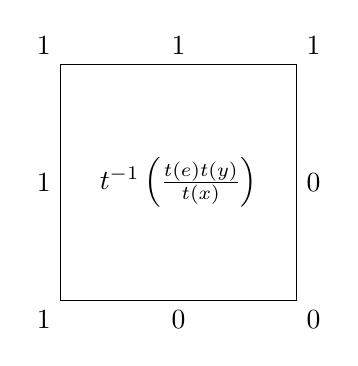
\begin{tikzpicture}[xscale=3, yscale=3]
			\draw (0,0) rectangle (1,1);
			\node [above right] at (1,1) {1} ;
			\node [below right] at (1,0) {0};
			\node [below left] at (0,0) {1};
			\node [above left] at (0,1) {1};
			\node [above] at (0.5,1) {1};
			\node [below] at (0.5,0) {$0$};
			\node [left] at (0,0.5) {1};
			\node [right] at (1,0.5) {$0$};
			\node at (0.5,0.5) {$t^{-1} \left(\frac{t(e)t(y)}{t(x)}\right)$};
		\end{tikzpicture}
	\end{subfigure}%
	\vspace{0.5cm}
	\newline
	\begin{subfigure}[t]{.3\textwidth}
		\centering
		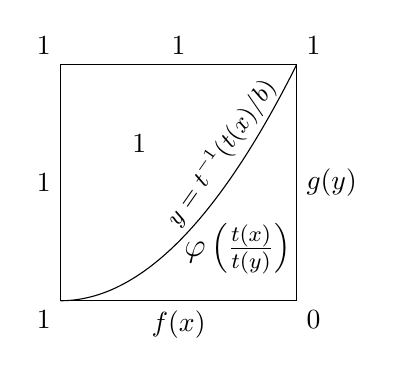
\begin{tikzpicture}[xscale=3, yscale=3]
			\draw (0,0) rectangle (1,1);
			\draw[domain=0:1,smooth,variable=\x,samples=200] plot (\x,{\x*\x});
			\node [above,rotate=55] at (0.76,0.57) {\small $y=t^{-1}(t(x)/b)$};
			\node [above right] at (1,1) {1} ;
			\node [below right] at (1,0) {0};
			\node [below left] at (0,0) {1};
			\node [above left] at (0,1) {1};
			\node [above] at (0.5,1) {1};
			\node [below] at (0.5,0) {$f(x)$};
			\node [left] at (0,0.5) {1};
			\node [right] at (1,0.5) {$g(y)$};
			\node at (1/3,2/3) {$1$};
			\node at (3/4,0.22) {\large $\varphi \left( \frac{t(x)}{t(y)} \right)$};
		\end{tikzpicture}
	\end{subfigure}%
	\hspace{0.5cm}
	\begin{subfigure}[t]{.3\textwidth}
		\centering
		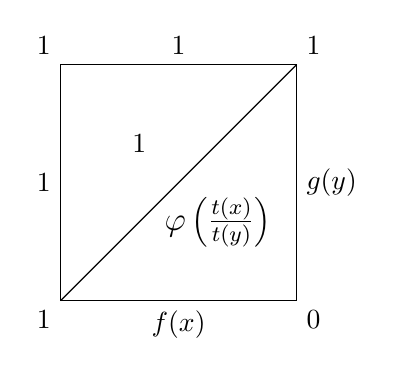
\begin{tikzpicture}[xscale=3, yscale=3]
			\draw (0,0) rectangle (1,1);
			\draw (0,0) -- (1,1);
			\node [above right] at (1,1) {1} ;
			\node [below right] at (1,0) {0};
			\node [below left] at (0,0) {1};
			\node [above left] at (0,1) {1};
			\node [above] at (0.5,1) {1};
			\node [below] at (0.5,0) {$f(x)$};
			\node [left] at (0,0.5) {1};
			\node [right] at (1,0.5) {$g(y)$};
			\node at (1/3,2/3) {$1$};
			\node at (2/3,1/3) {\large$\varphi \left( \frac{t(x)}{t(y)} \right)$};
		\end{tikzpicture}
	\end{subfigure}%
	\caption[Schema of the structure of strict $T$-power invariant implications that satisfy \NP, \NPe, \IP and \OP]{From left to right and from top to bottom, sketch of the structure of strict $T$-power invariant implications that satisfy \NP, \NPe, \IP and \OP. For \IP we have considered the case when $\varphi(w)=1$ if and only if $w \in [b,+\infty)$ with $b \in (0,1)$.}
	\label{fig:strict:structure(NP),(IP),(OP)}
\end{figure}
% Exchange principle %
Now, we consider the exchange principle. In order to characterize all strict $T$-power implications that satisfy \EP let us first prove some previous lemmas. First, the next result shows that if $f(x)=g(y)=0$ for all $x,y \in (0,1)$, then the corresponding \STP must have trivial 1-region in order to satisfy \EP.
% Previous lemmas %
% Lemma 1 %
\begin{lemma}\label{lem:strict:noreg1} Let $\IT$ be a strict $T$-power invariant implication. If $f(x)=g(y)=0$ for all $x,y \in (0,1)$ and there exists $(x,y) \in (0,1)^2$ such that $\IT(x,y)=1$, then $\IT$ does not satisfy \EP.
\end{lemma}
\begin{proof} Let us consider $\IT$ a strict $T$-power invariant implication with $f(x)=g(y)=0$ for all $x,y \in (0,1)$ and $x_0,y_0 \in (0,1)$ such that $\IT(x_0,y_0)=1$. We have that
	$$ \IT(1,\IT(x_0,y_0))=\IT(1,1)=1,$$
	$$ \IT(x_0,\IT(1,y_0)) = \IT(x_0,g(y_0)) =\IT(x_0,0)=f(x_0)=0,$$
	and since $\IT(1,\IT(x_0,y_0)) \not = \IT(x_0,\IT(1,y_0))$, $\IT$ does not satisfy \EP.
\end{proof}
The following lemma plays a key part when studying the exchange principle in the strict case. The result proves that if \IT is a \STP which satisfies \EP and has a $\varphi$ which is constant to $k\in(0,1)$ in some subinterval of $(0,+\infty)$, then necessarily $\varphi$ is constant to $k$ in the whole interval $(0,+\infty)$. Thanks to this lemma we know that given a non-strictly increasing $\varphi$, if $\IT$ is a \STP satisfying \EP, then $\IT$ must be constant in $(0,1)^2$.
% Lemma 2 %
\begin{lemma}\label{lem:strict:phi_const} Let \IT be a \STP. If $\IT$ satisfies \EP and there exists a constant $k \in (0,1)$ such that $\varphi(x)=k$ for all $x \in (a,b)$  with $0<a<b<+\infty$, then $\varphi(w)=k$ for all $w \in (0,+\infty)$.
\end{lemma}
\begin{proof} Consider \IT a \STP, a constant $k \in (0,1)$ and a non-empty interval $(a,b) \subseteq (0,+\infty)$ such that $\varphi(w)=k$ for all $w \in (a,b)$. Let us consider a $z_0 \in (0,1)$, we have that
	$$\varphi \left(\frac{t(x)}{t(z_0)}\right) =k, \quad \text{for all } x \in (t^{-1}(bt(z_0)),t^{-1}(at(z_0))).$$
	Now, for $x,y \in (t^{-1}(bt(z_0)),t^{-1}(at(z_0)))$, due to the fact that $\IT$ satisfies \EP we have that
	\begin{eqnarray*}
	\varphi \left(\frac{t(y)}{t(k)}\right) &=&\IT(y,k)=\IT(y,\IT(x,z_0))=\IT(x,\IT(y,z_0))\\
	 &=& \IT(x,k) = \varphi \left(\frac{t(x)}{t(k)}\right).
	\end{eqnarray*}
	Therefore, $\varphi$ is a constant function in the interval $ \frac{t(z_0)}{t(k)}(a,b)$. Now, we will prove that $\varphi(w)=k$ for all $w \in (0,+\infty)$ by taking two steps:
	\begin{enumerate}
		\item Let us consider $z_0 \in (k,t^{-1}(\frac{a}{b}t(k)))$, by the argument above we know that $\varphi$ is constant in $\frac{t(z_0)}{t(k)}(a,b)$. Now, we have that
		$$\frac{t(z_0)}{t(k)}a < \frac{t(k)}{t(k)}a=a,$$
		$$\frac{t(z_0)}{t(k)}b > \frac{a}{b} \frac{t(k)}{t(k)}b=a.$$
		Thus, $\frac{t(z_0)}{t(k)}(a,b)$ has non-empty intersection with $(a,b)$ which implies that $\varphi(w)=k$ in the interval $ \left(\frac{t(z_0)}{t(k)}a,b\right)$. Let us define the following family of intervals
		$$(a_n,b)=\left( \left(\frac{t(z_0)}{t(k)}\right)^na,b\right), \quad \text{for all } n \in \NN.$$
		Since
		$$a_n=\frac{t(z_0)}{t(k)}a_{n-1}<a_{n-1},$$
		$(a_n,b)$ has non-empty intersection with $(a_{n-1},b)$ and we have that $\varphi(w)=k$ for all $w \in (a_n,b)$ and $n \in \NN$. Now, since $\frac{t(z_0)}{t(k)}<1$ we get that
		$$ \lim_{n \to +\infty}a_n = \lim_{n \to +\infty} \left(\frac{t(z_0)}{t(k)}\right)^na=0,$$
		and we obtain that $\varphi(w)=k$ for all $w \in (0,b)$.
		\item On the other hand, by considering $z_0 \in (t^{-1}(\frac{b}{a}t(k)),k)$ we obtain that $\varphi$ is constant in $\frac{t(z_0)}{t(k)}(a,b)$ where this interval has non-empty intersection with $(a,b)$ since
		$$ \frac{t(z_0)}{t(k)}a < \frac{b}{a}\frac{t(k)}{t(k)}a =b,$$
		$$ \frac{t(z_0)}{t(k)}b> \frac{t(k)}{t(k)}b=b.$$
		In a similar manner as in the previous case we obtain that $\varphi(w)=k$ for all $w \in (a,b_n)$ where $b_n=\left(\frac{t(z_0)}{t(k)}\right)^nb$ for all $n \in \NN$. Since $\frac{t(z_0)}{t(k)}>1$ we have that
		$$\lim_{n \to +\infty} b_n = \lim_{n \to +\infty} \left(\frac{t(z_0)}{t(k)}\right)^nb = +\infty,$$
		and we obtain that $\varphi(w)=k$ for all $w \in (a,+\infty)$.
	\end{enumerate}
Consequently, we have proved that $\varphi(w)=k$ for all $w \in (0,+\infty)$.
\end{proof}
Finally, the next lemma shows that if  a \STP \IT satisfies the exchange principle, then $g$ is the identity function in the image of $f$ except for 0 and 1.
% Lemma 3 %
\begin{lemma}\label{lem:strict:g(EP)} Let $\IT$ be a strict $T$-power invariant implication. If $\IT$ satisfies \EP then $g(y)=y$ for all $y \in \Ima f \setminus \{0,1\}$.
\end{lemma}
\begin{proof} Since $\IT$ satisfies \EP, for all $x \in(0,1)$ such that $f(x) \in (0,1)$ we have that
	$$f(x)=\IT(x,0)=\IT(x,\IT(1,0))=\IT(1,\IT(x,0))=\IT(1,f(x))=g \circ f(x).$$
\end{proof}
% Main result %
Thanks to the previous lemmas, we now prove that there are only five possible configurations of strict $T$-power invariant implications that result in functions satisfying \EP. In Figure \ref{fig:strict:solutions(EP)} we can see that only Structure (i) corresponds to a fuzzy implication function that is not constant in $(0,1)^2$.

\begin{proposition}\label{prop:strict:(EP)} Let $\IT$ be a strict $T$-power invariant implication. Then  $\IT$ satisfies \EP if and only if one of the following conditions hold:
	\begin{enumerate}[label=(\roman*)]
		\item Let $C \in (0,+\infty)$, then $\varphi(w)=t^{-1}\left( \frac{C}{w} \right)$ for all $w \in(0,+\infty)$ and $f(x)=g(y)=0$ for all $x,y \in (0,1)$.
		\item Let $k \in [0,1]$, then $\varphi(w)=k$ for all $w \in (0,+\infty)$ and $f(x)=g(y)=0$ for all $x,y \in (0,1)$.
		\item Let $k \in (0,1]$, then $\varphi(w)=k$ for all $w\in (0,+\infty)$ and one of the following conditions holds:
		\begin{enumerate}
			\item $f(x)=\left\{ \begin{array}{ll}
				k &   \text{if }   x \in A, \\
				0 &  \text{if }   x \in (0,1)\setminus A,	\end{array}
			\right.$ where $A$ is $(0,a|$ with $ a \in (0,1)$ or $A=\emptyset$ and $\Ima g \subseteq (0,k]$.
			\item $f(x)=k$ for all $x\in(0,1)$ and $\Ima g \subseteq [0,k]$.
			\item $\Ima f \subseteq (0,k]$, $\Ima g \subseteq (0,k]$ and $g(y)=y$ for all $y \in \Ima f \setminus \{1\}$.
		\end{enumerate}
		Moreover, if $k < 1$, $g$ must additionally satisfy $g(k)=k$.
	\end{enumerate}
\end{proposition}
\begin{proof}
	Assume that $\IT$ satisfies \EP, we distinguish between different cases depending on additional properties of $\varphi$, $f$ and $g$.
	\begin{enumerate}
		\item[Case 1.] $\varphi$ is strictly increasing. By definition we know that
		$$\IT(x,x)=\varphi(1), \quad \text{for all } x \in(0,1),$$
		with $\varphi(1) \in (0,1)$. Then, for all $x,y \in (0,1)$ we have that
		$$\IT(x,\IT(y,y)) =\IT(x,\varphi(1)) = \varphi \left(\frac{t(x)}{t\circ \varphi(1)}\right),$$
		$$\IT(y,\IT(x,y)) =\IT\left(y,\varphi\left(\frac{t(x)}{t(y)}\right)\right) = \varphi \left(\frac{t(y)}{t \circ \varphi \left(\frac{t(x)}{t(y)}\right)}\right).$$
		Since $\IT$ satisfies \EP and $\varphi$ is a strictly increasing function, we obtain that
		$$ \frac{t(x)}{t\circ \varphi (1)} = \frac{t(y)}{t \circ \varphi \left(\frac{t(x)}{t(y)}\right)} \Rightarrow \varphi \left(\frac{t(x)}{t(y)}\right) = t^{-1}\left(\frac{t(y)\cdot t \circ \varphi (1)}{t(x)}\right).$$
		Notice that given a $w \in (0,+\infty)$, we can find $x,y \in (0,1)$ such that $\frac{t(x)}{t(y)}=w$. Thus,
		$$ \varphi(w)=t^{-1}\left(\frac{C}{w}\right),$$
		for all $w \in (0,+\infty)$ where $C \in (0,+\infty)$ . Now, since
		$$\lim_{w \to 0^+} \varphi (w) = \lim_{w \to 0^+} t^{-1}\left(\frac{C}{w}\right) =t^{-1}(+\infty)=0=\varphi(0),$$
		we have that $\varphi$ is continuous on $w=0$ and by (i)-Proposition \ref{prop:strict:continuity} necessarily $f(x)=g(y)=0$ for all $ x,y\in (0,1)$.
		\item[Case 2.] If $\varphi$ is not strictly increasing, then it is constant in some interval $(a,b) \subseteq (0,+\infty)$ with $a<b$. Let us consider different subcases depending on the value of such constant.
		\begin{itemize}
			\item If $\varphi(w)=k$ for all $w \in (a,b)$ with $k \in (0,1)$, by Lemma \ref{lem:strict:phi_const} we have that $\varphi(w)=k$ for all $w \in (0,+\infty)$.
			\item If $\varphi(w)=1$ for all $w \in (a,b)$, then since $\varphi$ is an increasing mapping we have that $\varphi(w)=1$ for all $w \in (a,+\infty)$. By Lemma \ref{lem:strict:noreg1} we know that there exists $x\in(0,1)$ such that $f(x)$ or $g(x)>0$ and consequently, by Condition (\ref{eq:strict:TPowerInv:MonotonicityCond}),  $\varphi(w)>0$ for all $w \in (0,+\infty)$. Consider $w_0 \in (0,a]$ such that $\varphi(w_0) \in (0,1)$. Now, by choosing $x_0,y_0,z_0 \in (0,1)$ fulfilling that $y_0 > t^{-1}(w_0t\circ \varphi(w_0))$, $z_0 > t^{-1}\left(\frac{t(y_0)}{a}\right)$ and $x_0=t^{-1}(w_0t(z_0))$ we have that
			$$\IT(x_0,\IT(y_0,z_0))=\IT\left(x_0,\varphi\left(\frac{t(y_0)}{t(z_0)}\right)\right) =\IT(x_0,1)=1,$$
			$$ \IT(y_0,\IT(x_0,z_0))=\IT(y_0,\varphi(w_0))=\varphi\left(\frac{t(y_0)}{t\circ\varphi(w_0)}\right) \leq \varphi(w_0)<1,$$
			which contradicts the fact that $\IT$ satisfies \EP. Therefore $\varphi(w)=1$ for all $w \in (0,+\infty)$.
			\item If $\varphi(w)=0$ for all $w \in (a,b)$, then since $\varphi$ is an increasing mapping  we have that $\varphi(w)=0$ for all $w \in (0,b)$. Since $\varphi$ is continuous on $w=0$, by (i)-Proposition \ref{prop:strict:continuity}, we have that $f(x)=g(y)=0$ for all $x,y \in (0,1)$. Consider a $w_0 \in [b,+\infty)$ such that $\varphi(w_0) \in (0,1)$ and $x_0,y_0,z_0 \in (0,1)$ fulfilling that $y_0 < t^{-1}(w_0 t\circ \varphi(w_0))$, $ z_0 < t^{-1}\left(\frac{t(y_0)}{b}\right)$ and $x_0=t^{-1}(w_0t(z_0))$, we obtain that
			$$\IT(x_0,\IT(y_0,z_0))=\IT\left(x_0,\varphi \left(\frac{t(y_0)}{t(z_0)}\right)\right)=\IT(x_0,0)=f(x_0)=0,$$
			$$\IT(y_0,\IT(x_0,z_0))=\IT(y_0,\varphi(w_0))=\varphi \left(\frac{t(y_0)}{t\circ\varphi(w_0)}\right) \geq \varphi(w_0)>0,$$
			which contradicts the fact that $\IT$ satisfies \EP. Thus, $\varphi(w)=0$ for all $w \in (0,+\infty)$.
		\end{itemize}
		Then, we have proved that if $\varphi$ is not strictly increasing then it is constant in $(0,+\infty)$. Now, let us again consider different cases depending on the values of such constant.
		\begin{itemize}
			\item If $\varphi(w)=0$ for all $w \in (0,+\infty)$, then by (i)-Proposition \ref{prop:strict:continuity} we have that $f(x)=g(y)=0$ for all $x,y \in (0,1)$. This situation corresponds to Case (ii) with $k=0$.
			\item If $\varphi(w)=k$ for all $w \in (0,+\infty)$ with $k \in (0,1]$. By Condition (\ref{eq:strict:TPowerInv:MonotonicityCond}) we know that $\Ima f \subseteq [0,k]$ and $\Ima g \subseteq [0,k]$, and by Lemma \ref{lem:strict:g(EP)} we have that $g(y)=y$ for all $y \in \Ima f \setminus \{0,1\}$. Now, to see that the only possible cases are (ii), (iii)-(a), (iii)-(b) or (iii)-(c) first let us prove three facts:
			\begin{enumerate}
				\item[\bf (F1)] \textbf{If $k < 1$ and $g(y_0) \in (0,k]$ for some $y_0 \in (0,1)$, then $g(k)=k$.} Let us consider $k < 1$ and a $y_0 \in (0,1)$ such that $g(y_0) \in (0,k]$ then 
				\begin{eqnarray*}
				g(k) &=& \IT(1,k)=\IT(1,\IT(y_0,y_0))=\IT(y_0,\IT(1,y_0)) \\
				&=&\IT(y_0,g(y_0))=k,
				\end{eqnarray*}
				and we obtain that $g(k)=k$.
				\item[\bf (F2)] \textbf{If $f$ is not equal to the constant function $k$ and $g$ satisfies that $g(k)=k$ when $k<1$, then $g(y)>0$ for all $y \in (0,1)$.}
				Let us consider that there exists an $x_0 \in (0,1)$ such that $f(x_0) \in [0,k)$ and a $z_0 \in (0,1)$ such that $g(z_0)=0$. Then,
				$$\IT(x_0,\IT(1,z_0))=\IT(x_0,g(z_0)) =\IT(x_0,0)=f(x_0)\in [0,k),$$
				$$ \IT(1,\IT(x_0,z_0))=\IT(1,k)=\left\{ \begin{array}{ll}
					1 &   \text{if }   k=1, \\
					g(k) & \text{if }k < 1,
				\end{array}
				\right.=k,$$
				which contradicts the fact that $\IT$ satisfies \EP. Therefore, if there exists an $x_0 \in (0,1)$ such that $f(x_0)\in [0,k)$ and $g$ satisfies that $g(k)=k$ when $k<1$, we have proved that $\Ima g \subseteq (0,k]$.
				\item[\bf (F3)]\textbf{If $f$ values 0 at some point then the only possible values of $f$ are 0 or $k$.} Let us consider a $x_0 \in (0,1)$ such that $f(x_0)=0$ and $y_0 \in (0,1)$ with $f(y_0) \in (0,k)$. Then,
				$$\IT(x_0,\IT(y_0,0))=\IT(x_0,f(y_0))=k,$$
				$$\IT(y_0,\IT(x_0,0))=\IT(y_0,0)=f(y_0) \in (0,k),$$
				and we again arrive to contradiction because $\IT$ satisfies \EP. Therefore, if there exists an $x_0 \in (0,1)$ such that $f(x_0)=0$ we have that $\Ima f \subseteq \{0,k\}$.
			\end{enumerate}
			Having said this, let us now argue why (ii), (iii)-(a), (iii)-(b) or (iii)-(c) are the only possible cases. In order to do so, we distinguish between several situations depending on the possible values of the function $f$.
			\begin{itemize}
				\item If $f(x)=0$ for all $x \in (0,1)$ then we distinguish between two cases:
				\begin{itemize}
					\item If $g(y)=0$ for all $y \in (0,1)$ we are in Case (ii) with $k \in (0,1]$.
					\item If $g(y_0) > 0 $ for some $y_0 \in (0,1)$, by {\bf (F1)} we have that $g(k)=k$ whenever $k < 1$ and by {\bf (F2)} $\Ima g \subseteq (0,k]$. Then, we are in Case (iii)-(a) with $A=\emptyset$.
				\end{itemize}
				\item If $0 \in \Ima f$ but there exists an $x_0 \in (0,1)$ such that $f(x_0) \in (0,k]$. Then, by {\bf (F2)} $\Ima g \subseteq (0,k]$, and when $k < 1$, by Lemma \ref{lem:strict:g(EP)} we know that $g(k)=k$. Therefore, we are in Case (iii)-(a) with $A \not = \emptyset$.
				\item If $0 \not \in \Ima f$ we distinguish between two cases:
				\begin{itemize}
					\item If $f(x)=k$ for all $x \in (0,1)$, by Lemma \ref{lem:strict:g(EP)} we know that $g(k)=k$ whenever $k < 1$ and we are in Case (iii)-(b).
					\item If $f(x_0) \in (0,k)$ for some $x_0 \in (0,1)$, by Lemma \ref{lem:strict:g(EP)} $g(f(x_0))=f(x_0)$ and by {\bf (F1)} $g(k)=k$ whenever $k < 1$. Finally, by {\bf (F2)} $\Ima g \subseteq (0,k]$ and we are in Case (iii)-(c).
				\end{itemize}
			\end{itemize}
		\end{itemize}
	\end{enumerate}
	For the reverse implication, we have to prove that the choices for $f$, $g$ and $\varphi$ gathered in (i), (ii) and (iii) represent strict $T$-power invariant implications that satisfy \EP. Notice that by the properties of fuzzy implication functions, it is enough to prove \EP for values $x,y \in (0,1]$ with $x<y$ and $z \in [0,1).$ We will provide the details of case (iii)-(c), which is the most complex case, leaving as a matter of straightforward computation the other cases. Consider $\varphi$, $f$ and $g$ fulfilling conditions in (iii)-(c). Then,
	\begin{eqnarray*}
	\IT(x,\IT(y,z)) 
	&=&
	\left\{ \begin{array}{ll}
		\IT(x,0) &   \text{if }   y=1 \text{ and } z=0, \\[5pt]
		\IT(x,f(y)) & \text{if } y\in (0,1) \text{ and } z =0,\\[5pt]
		\IT(x,g(z)) & \text{if } y=1 \text{ and } z \in (0,1),\\[5pt]
		\IT(x,k) & \text{otherwise,}
	\end{array}
	\right. \\
	&=&
	\left\{ \begin{array}{ll}
		f(x) &   \text{if }   y=1 \text{ and } z=0, \\
		k & \text{otherwise.}
	\end{array}
	\right.
	\end{eqnarray*}
	Let us distinguish two cases depending on the value of the constant $k$:
	\begin{itemize}
		\item If $k\in (0,1)$, then $g(k)=k$ and
		\begin{eqnarray*}
			\IT(y,\IT(x,z)) &=& 
			\left\{ \begin{array}{ll}
				\IT(y,f(x)) &   \text{if }   z=0, \\[5pt]
				\IT(y,k) & \text{if } z \in (0,1),
			\end{array}
			\right. \\
			&=&
			\left\{ \begin{array}{ll}
				g \circ f(x) &   \text{if }   y=1 \text{ and } z=0, \\
				g(k) & \text{if } y=1 \text{ and } z \in (0,1)\\
				k & \text{otherwise,}
			\end{array}
			\right. \\
			&=&
			\left\{ \begin{array}{ll}
				f(x) &   \text{if }   y=1 \text{ and } z=0, \\
				k & \text{otherwise.}
			\end{array}
			\right.
		\end{eqnarray*}
		\item If $k=1$, then
		\begin{eqnarray*}
			\IT(y,\IT(x,z)) &=& 
			\left\{ \begin{array}{ll}
				\IT(y,f(x)) &   \text{if }   z=0, \\[5pt]
				\IT(y,1) & \text{if } z \in (0,1),
			\end{array}
			\right. \\
			&=&
			\left\{ \begin{array}{ll}
				g \circ f(x) &   \text{if }   y=1, z=0 \text{ and } f(x) \in (0,1), \\
				1 & \text{if } y=1, z=0 \text{ and } f(x)=1,\\
				1 & \text{otherwise}
			\end{array}
			\right. \\
			&=&
			\left\{ \begin{array}{ll}
				f(x) &   \text{if }   y=1 \text{ and } z=0, \\
				1 & \text{otherwise.}
			\end{array}
			\right.
		\end{eqnarray*}	
	\end{itemize}
\end{proof}
% Figure -- Structures (EP) %
\begin{figure}[t]
	\centering
	\begin{subfigure}[t]{0.25\linewidth}\vspace{0pt}
		\flushleft
		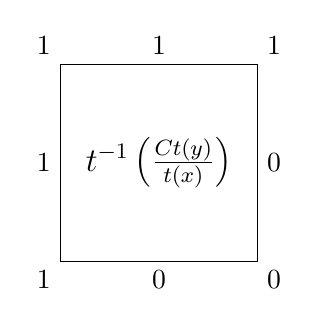
\begin{tikzpicture}[xscale=2.5, yscale=2.5]
			\draw (0,0) rectangle (1,1);
			\node [above right] at (1,1) {1} ;
			\node [below right] at (1,0) {0};
			\node [below left] at (0,0) {1};
			\node [above left] at (0,1) {1};
			\node [above] at (0.5,1) {1};
			\node [below] at (0.5,0) {0};
			\node [left] at (0,0.5) {1};
			\node [right] at (1,0.5) {0};
			\node at (0.5,0.5) {\large $t^{-1} \left( \frac{C t(y)}{t(x)} \right)$};
		\end{tikzpicture}
		\caption*{Case (i)~~~~~}	
	\end{subfigure}
	\begin{subfigure}[t]{0.25\linewidth}\vspace{0pt}
		\flushleft
		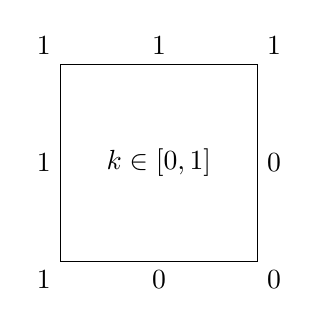
\begin{tikzpicture}[xscale=2.5, yscale=2.5]
			\draw (0,0) rectangle (1,1);
			\node [above right] at (1,1) {1} ;
			\node [below right] at (1,0) {0};
			\node [below left] at (0,0) {1};
			\node [above left] at (0,1) {1};
			\node [above] at (0.5,1) {1};
			\node [below] at (0.5,0) {0};
			\node [left] at (0,0.5) {1};
			\node [right] at (1,0.5) {0};
			\node at (0.5,0.5) {$k \in [0,1]$};
		\end{tikzpicture}
		\caption*{Case (ii)~~~~~}
	\end{subfigure}
	\begin{subfigure}[t]{0.25\linewidth}\vspace{0pt}
		\flushleft
		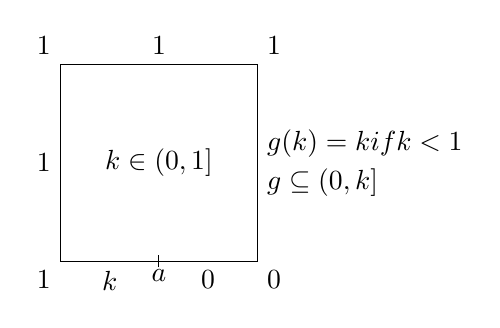
\begin{tikzpicture}[xscale=2.5, yscale=2.5]
			\draw (0,0) rectangle (1,1);
			\node [above right] at (1,1) {1} ;
			\node [below right] at (1,0) {0};
			\node [below left] at (0,0) {1};
			\node [above left] at (0,1) {1};
			\node [above] at (0.5,1) {1};
			\node [left] at (0,0.5) {1};
			\node at (0.5,0.5) {$k\in (0,1]$};
			\node [right] at (1,0.6) {$g(k)=k \text{ if } k < 1$};
			\node [right] at (1,0.4) {$\Ima g \subseteq (0,k]$};
			\draw (0.5,-0.03)--(0.5,0.03);
			\node at (0.5,-0.07) {$a$};
			\node [below] at (1/4,0) {$k$};
			\node [below] at (3/4,0) {$0$};
		\end{tikzpicture}
		\caption*{Case (iii)-(a)~~~~}		
	\end{subfigure}
	\begin{subfigure}[t]{0.45\linewidth}\vspace{0pt}
		~~~~~~~~~~~~~~~~~~
		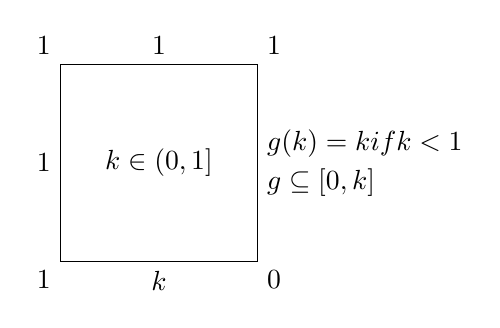
\begin{tikzpicture}[xscale=2.5, yscale=2.5]
			\draw (0,0) rectangle (1,1);
			\node [above right] at (1,1) {1} ;
			\node [below right] at (1,0) {0};
			\node [below left] at (0,0) {1};
			\node [above left] at (0,1) {1};
			\node [above] at (0.5,1) {1};
			\node [left] at (0,0.5) {1};
			\node at (0.5,0.5) {$k \in (0,1]$};
			\node [right] at (1,0.6) {$g(k)=k \text{ if } k < 1$};
			\node [right] at (1,0.4) {$\Ima g \subseteq [0,k]$};
			\node [below] at (0.5,0) {$k$};
		\end{tikzpicture}
		\caption*{~~Case (iii)-(b)}	
	\end{subfigure}
	\hspace{1.25cm}
	\begin{subfigure}[t]{0.45\linewidth}\vspace{0pt}
		\flushright
		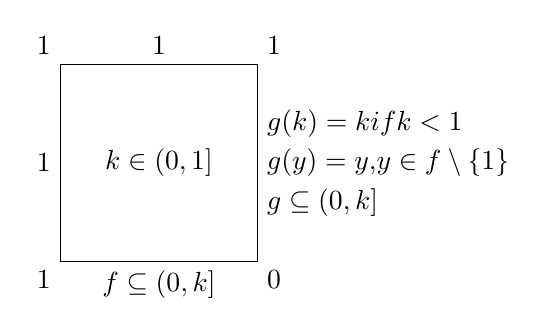
\begin{tikzpicture}[xscale=2.5, yscale=2.5]
			\draw (0,0) rectangle (1,1);
			\node [above right] at (1,1) {1} ;
			\node [below right] at (1,0) {0};
			\node [below left] at (0,0) {1};
			\node [above left] at (0,1) {1};
			\node [above] at (0.5,1) {1};
			\node [left] at (0,0.5) {1};
			\node at (0.5,0.5) {$k \in (0,1]$};
			\node [below] at (0.5,0) {$\Ima f \subseteq (0,k]$};
			\node [right] at (1,0.7) {$g(k)=k \text{ if } k < 1$};
			\node [right] at (1,0.5) {$g(y)=y \text{, } y \in \Ima f \setminus \{1\}$};
			\node [right] at (1,0.3) {$\Ima g \subseteq (0,k]$};
		\end{tikzpicture}
		\caption*{Case (iii)-(c)~~~~~~~~~~~~~~~~~~~~~~~~~~~}	
	\end{subfigure}
	\caption[Schema of the structure of strict $T$-power invariant implications that satisfy \EP.]{Schema of the structure of strict $T$-power invariant implications that satisfy \EP defined in Proposition \ref{prop:strict:(EP)}. In Case (iii)-(a) we have considered an $a \in (0,1)$.}
	\label{fig:strict:solutions(EP)}
\end{figure}

\begin{remark}\label{remark:(NPe)}
	It is interesting to notice that the solution of \NPe described in Proposition \ref{prop:strict:(NPe)} is the same as the Case (i) in Proposition \ref{prop:strict:(EP)} where $C=t(e)$. Therefore, the members of the family of strict $T$-power invariant implications that satisfy \NPe, also satisfy \EP.
\end{remark}
\begin{remark}\label{remark:preferenceimplication}
	Let us point out that one of the solutions in Proposition \ref{prop:strict:(EP)} has an unexpected relation with another family of fuzzy implication functions defined independently from the invariance property. In \cite{Baczynski2020B} Baczy\'{n}ski and Dombi introduced the preference implication as the fuzzy implication function which is the solution of the four basic distributive equations with respect to the operators of the pliant system. The preference implication $p_{\nu}:[0,1]^2 \to [0,1]$ is defined as
	$$
	p_{\nu}(x,y) =
	\left\{ \begin{array}{ll}
		1 &   \text{if }  (x,y) \in \{(0,0),(1,1)\}, \\[5pt]
		t^{-1}\left(t(\nu)\frac{t(y)}{t(x)}\right) & \text{otherwise},
	\end{array}
	\right.
	$$
	where $t$ is an additive generator of a strict t-norm and $\nu \in (0,1)$. In view of the results in Proposition \ref{prop:strict:(EP)}, it is clear that the preference implication corresponds to Case (i) with $C=t(\nu)$ and then it is included in the subfamily of strict $T$-power invariant implications that satisfy \EP. Thus, from our study it can be derived that the preference implication also satisfies the invariance property with respect to the strict t-norm generated by $t$, and from the study in \cite{Baczynski2020B} we can affirm that the only strict $T$-power invariant implication that satisfies \EP and it is not constant in $(0,1)^2$ also satisfies the four distributivities with respect to the corresponding operators of the pliant system.
\end{remark}

% Example -- (EP) %
\begin{example}\label{example:strict:(EP)} Let us consider $t(s)=\frac{1-s}{s}$ for all $s \in [0,1]$. The corresponding strict $T$-power invariant implication that satisfies \EP and is non-constant in $(0,1)^2$ is given by
	$$I_{3}(x,y) =\left\{ \begin{array}{ll}
		1 & \text{if } (x=0 \text{ and } y \in [0,1]) \text{ and } (x \in (0,1] \text{ and } y=1),\\
		0 &   \text{if }   (x \in (0,1) \text{ and } y=0) \text{ and } ( x = 1 \text{ and } y\in [0,1)), \\
		\frac{(1-x)y}{Cx-Cxy+y-xy} &  \text{otherwise},
	\end{array}
	\right.
	$$
	where $C\in (0,+\infty)$. Note that $I_3$ corresponds to the solution given in {(i)-Proposition~\ref{prop:strict:(EP)}}. In Figure \ref{exfig:strict:(EP)} we can see the plots of some members of this family of fuzzy implication functions for $C=1$, $C=10$ and $C=100$.
\end{example}
\begin{figure}[t]
	\centering
	\begin{subfigure}{.3\textwidth}
		\centering
		\includegraphics[width=.8\linewidth]{K1.pdf}
		\caption{$C=1$}
	\end{subfigure}%
	\begin{subfigure}{.3\textwidth}
		\centering
		\includegraphics[width=.8\linewidth]{K10.pdf}
		\caption{$C=10$}
	\end{subfigure}
	\begin{subfigure}{.3\textwidth}
		\centering
		\includegraphics[width=.8\linewidth]{K100.pdf}
		\caption{$C=100$}
	\end{subfigure}
	\caption[Plots of three strict $T$-power invariant implications that satisfy \EP.]{Plots of fuzzy implication functions given in Example \ref{example:strict:(EP)} for $C=1$, $C=10$ and $C=100$.}
	\label{exfig:strict:(EP)}
\end{figure}
% Law of importation %
We now turn to study the law of importation. It is well known, that \LI implies \EP but the reverse implication does not hold in general. Thus, to study \LI we can use as starting point the five configurations in Proposition \ref{prop:strict:(EP)}. Before characterizing all strict $T$-power implications satisfying \LI let us prove the following lemma which remarks some interesting properties such as if \IT satisfies \LI with respect to some t-norm $T^*$, then $\IT$ is constant in $(0,1)^2$, $g$ is idempotent in its image except for 0 and 1 (see Lemma \ref{lem:idempotentfunctions} for a characterization of these type of functions) and if $\IT$ has trivial 1-region then necessarily $T^*$ is a positive t-norm (also called t-norm without zero-divisors), i.e., $T^*(x,y)=0$ if and only if $x=0$ or $y=0$.
% law of importation %
\begin{lemma}\label{lem:strict:(LI)} Let \IT be a \STP that satisfies \LI with respect to some t-norm $T^*$. The following statements hold:
	\begin{enumerate}[label=(\roman*)]
		\item $\IT$ is constant in $(0,1)^2$.
		\item If $\IT(x,y)=1 \Leftrightarrow (x=0 \text{ or } y=1$), then $T^*$ is a positive t-norm.
		\item $g(y)=y$ for all $y \in \Ima g\setminus \{0,1\}$.
	\end{enumerate}
\end{lemma}
\begin{proof} \hspace{0.5cm}
	\begin{enumerate}[label=(\roman*)]
		\item Let us prove that Case (i) in Proposition \ref{prop:strict:(EP)} does not satisfy \LI with respect to any t-norm $T^*$. Consider $x=1$, $y,z \in (0,1)$, we have that
		$$\IT(T^*(1,y),z)=\IT(y,z)\in(0,1),$$
		$$\IT(1,\IT(y,z))=g(\IT(y,z))=0.$$
		Thus, observing that all the other cases in Proposition \ref{prop:strict:(EP)} correspond to fuzzy implication functions which are constant in $(0,1)^2$ we obtain the result.
		\item Consider that there exist $x_0, y_0 \in (0,1)$ such that $T^*(x_0,y_0)=0$, then for $z_0 \in (0,1)$ we have that
		$$\IT(T^*(x_0,y_0),z_0)=\IT(0,z_0)=1,$$
		$$\IT(x_0,\IT(y_0,z_0))<1.$$
		Then, we arrive to contradiction with the fact that $\IT$ satisfies \LI with respect to $T^*$.
		\item Let us assume $x=y=1$ and $z \in (0,1)$, then
		\begin{eqnarray*}
		\IT(1,\IT(1,z)) &=&
		\left\{ \begin{array}{ll}
			\IT(1,0)&\text{if }z=0, \\[3pt]
			\IT(1,g(z))&\text{if }z \in (0,1),\\[3pt]
			\IT(1,1)&\text{if }z=1,
		\end{array}
		\right. \\
		&=&
		\left\{ \begin{array}{ll}
			0&\text{if }z=0 \text{ or } (z \in (0,1) \text{ and } g(z)=0), \\
			g \circ g(z)&\text{if }z \in (0,1) \text{ and } g(z) \in (0,1),\\
			1&\text{if }z=1 \text{ or } (z \in(0,1) \text{ and } g(z)=1).
		\end{array}
		\right.
		\end{eqnarray*}
		$$
		\IT(T^*(1,1),z)
		=
		\IT(1,z)
		=
		\left\{ \begin{array}{ll}
			0&\text{if }z=0, \\
			g(z)&\text{if }z \in (0,1),\\
			1&\text{if }z=1.
		\end{array}
		\right.
		$$
		Then, since $\IT$ satisfies \LI with respect to $T^*$, necessarily we have that $g\circ g(z)=g(z)$ for all $g(z) \in (0,1)$ with $z \in (0,1)$, that is equivalent to $g(y)=y$ for all $y \in \Ran g \setminus \{0,1\}$.
	\end{enumerate}
\end{proof}
Thanks to the above, the following proposition determines the three possibles configurations of strict $T$-power invariant implications that satisfy the law of importation with respect to some t-norm.
\begin{proposition}\label{prop:strict:(LI)} Let \IT be a \STP and $T^*$ a t-norm. Then $\IT$ satisfies \LI with respect to $T^*$ if and only if one of the following conditions hold:
	\begin{enumerate}[label=(\roman*)]
		\item $\varphi(w)=0$ for all $w \in (0,+\infty)$, $f(x)=g(y)=0$ for all $x,y \in (0,1)$ and $T^*$ is a positive t-norm.
		\item  Let $k \in (0,1]$, then $\varphi(w)=k$ for all $w \in (0,+\infty)$, $g(y)=y$ for all $y \in \Ima g \setminus \{0,1\}$, and one of the following conditions hold:
		\begin{enumerate}
			\item $f(x)=\left\{ \begin{array}{ll}
				k &   \text{if }   x \in A, \\
				0 &  \text{if }   x \in (0,1)\setminus A,	\end{array}
			\right.$ where $A$ is $(0,a|$ with $ a \in (0,1)$ or $A=\emptyset$, $T^*$ satisfies the following property
			$$T^*(x,y) \in (0,1]\setminus A \text{ if and only if } x,y \in (0,1]\setminus A$$
			and $\Ima g \subseteq (0,k]$.
			\item $0 \not \in \Ima f$, $f(x)=k$ for all $x \in \Ima T^*|_{(0,1)^2} \setminus \{0\}$, $g(y)=y$ for all $y \in \Ima f \setminus \{1\}$ and $\Ima g \subseteq [0,k]$ but $g(y) > 0$ for all $y \in (0,1)$ when $f$ is not a function constant to $k$.
		\end{enumerate}
		Moreover, if $k < 1$, $g$ must additionally satisfy $g(k)=k$ and $T^*$ must be a positive t-norm.
	\end{enumerate}
\end{proposition}
\begin{proof}
	Let \IT be a \STP which satisfies \LI with respect to a t-norm $T^*$. {By (i)-Lemma~\ref{lem:strict:(LI)}} we know that there exists some $k \in [0,1]$ such that $\varphi(w)=k$ for all $w \in (0,+\infty)$ and by (iii) that $g$ is idempotent in $\Ima g \setminus \{0,1\}$. Now, since we know that \LI $\Rightarrow$ \EP, then we only need to consider Cases (ii), (iii)-(a), (iii)-(b) and (iii)-(c) in Proposition \ref{prop:strict:(EP)}:
	\begin{description}
		\item[ Case (ii)] If $k=0$ we are in Case (i) of Proposition \ref{prop:strict:(LI)}. On the other hand, if $k \in (0,1]$ then \IT does not verify \LI with respect to any t-norm $T^*$ because for $x,z \in (0,1)$ we have that
		$$ \IT(T^*(x,1),z)=\IT(x,z)=k,$$
		$$\IT(x,\IT(1,z))=\IT(x,g(z))=\IT(x,0)=f(x)=0.$$
		\item[Case (iii)-(a)] Let us prove that in this case $T^*(x,y) \in (0,1] \setminus A \Leftrightarrow x,y \in (0,1] \setminus A$. Consider $x,y \in (0,1)\setminus A$ such that $T^*(x,y) \in A \cup \{0\}$, we have that
		$$\IT(T^*(x,y),0)=\left\{ \begin{array}{ll}
			k &   \text{if }   T^*(x,y) \in A, \\
			1 &  \text{if }   T^*(x,y)=0,	\end{array}
		\right. $$
		$$\IT(x,\IT(y,0))=\IT(x,0)=0,$$
		and we arrive to contradiction with the fact that $\IT$ satisfies \LI with respect to $T^*$. 		
		On the other hand, consider $T^*(x,y)\in (0,1]\setminus A$. Since $T^*(x,y) \leq \min\{x,y\}$ we have that $x,y \in (0,1] \setminus A$. This situation corresponds to (ii)-(a) in Proposition \ref{prop:strict:(LI)}.
		\item[Case (iii)-(b)] Notice that this case is contemplated in situation (ii)-(b) in Proposition \ref{prop:strict:(LI)}.
		\item[Case (iii)-(c)]  Let us prove that in this case $f(x)=k$ for all $x \in \Ima T^*|_{(0,1)^2} \setminus \{0\}$. Consider an $r \in \Ima T^*|_{(0,1)^2} \setminus \{0\}$ such that $T^*(x_0,y_0)=r$ with $(x_0,y_0)\in (0,1)^2$ and $f(r)<k$, then
		$$\IT(T^*(x_0,y_0),0)=f(T^*(x_0,y_0))=f(r)<k,$$
		$$\IT(x_0,\IT(y_0,0))=\IT(x_0,f(y_0))=k,$$
		which contradicts the fact that \IT satisfies \LI with respect to $T^*$. This situation corresponds to Case (ii)-(b) in Proposition \ref{prop:strict:(LI)}.
	\end{description}
	For the reverse implication, we have to prove that fuzzy implication functions described in (i), (ii)-(a) and (ii)-(b) satisfy \LI with respect to $T^*$. Since this step involves some tedious expressions, here we only present the details for Case (ii)-(b). Let $\varphi$, $f$, $g$ and $T^*$ fulfill conditions in (ii)-(b), then
	\begin{eqnarray*}
		\IT(T^*(x,y),z)&=&
		\left\{ \begin{array}{ll}
			0 &   \text{if }  T^*(x,y)=1 \text{ and } z=0, \\
			f(x) &  \text{if } x \in (0,1), y=1 \text{ and } z=0,\\
			f(y) & \text{if } x=1, y \in (0,1) \text{ and } z=0\\
			f(T^*(x,y)) & \text{if }x,y \in (0,1), T^*(x,y) \in (0,1) \text{ and } z=0,\\
			g(z) & \text{if } T^*(x,y)=1 \text{ and } z \in (0,1),\\
			1 & \text{if } T^*(x,y)=0 \text{ or } z =1,\\
			k & \text{otherwise,}
		\end{array} \right. \\
		&=&
		\left\{ \begin{array}{ll}
			0 &   \text{if }  x=y=1 \text{ and } z=0, \\
			f(x) &  \text{if } x \in (0,1), y=1 \text{ and } z=0,\\
			f(y) & \text{if } x=1, y \in (0,1) \text{ and } z=0,\\
			f(T^*(x,y)) & \text{if }x,y \in (0,1), T^*(x,y) \in (0,1) \text{ and } z=0,\\
			g(z) & \text{if } x=y=1 \text{ and } z \in (0,1),\\
			1 & \text{if } T^*(x,y)=0 \text{ or } z =1,\\
			k & \text{otherwise.}
		\end{array} \right.
	\end{eqnarray*}
	Let us distinguish two cases depending on the value of $k$:
	\begin{itemize}
		\item 	If $k \in (0,1)$ then
		\begin{eqnarray*}
			\IT(x,\IT(y,z)) &=&
			\left\{ \begin{array}{ll}
				\IT(x,0) &   \text{if }  y=1 \text{ and } z=0, \\[5pt]
				\IT(x,f(y)) &  \text{if } y \in (0,1) \text{ and } z=0,\\[5pt]
				\IT(x,g(z)) & \text{if } y=1 \text{ and } z \in (0,1),\\[5pt]
				\IT(x,1) & \text{if }y=0 \text{ or } z=1,\\
				k & \text{otherwise,}
			\end{array} \right. \\
			&=&
			\left\{ \begin{array}{ll}
				0 &   \text{if }  x=y=1 \text{ and } z=0, \\
				f(x) & \text{if }x\in(0,1), y=1 \text{ and } z=0, \\
				g \circ f(y) &  \text{if } x=1, y \in (0,1) \text{ and } z=0,\\
				g \circ g(z) & \text{if } x=y=1 \text{ and } z \in (0,1),\\
				1 & \text{if }x=0 \text{ or } y=0 \text{ or } z=1,\\
				k & \text{otherwise,}
			\end{array} \right. \\
			&=&
			\left\{ \begin{array}{ll}
				0 &   \text{if }  x=y=1 \text{ and } z=0, \\
				f(x) & \text{if }x\in(0,1), y=1 \text{ and } z=0, \\
				f(y) &  \text{if } x=1, y \in (0,1) \text{ and } z=0,\\
				g(z) & \text{if } x=y=1 \text{ and } z \in (0,1),\\
				1 & \text{if }x=0 \text{ or } y=0 \text{ or } z=1,\\
				k & \text{otherwise.}
			\end{array} \right.		 
		\end{eqnarray*}
		Since in this case we have that $g(k)=k$ and $T^*$ is a positive t-norm it is clear by the conditions in (ii)-(b) that \LI holds.	
		\item $k=1$
		\begin{eqnarray*}
			\IT(x,\IT(y,z)) &=&
			\left\{ \begin{array}{ll}
				0 & \text{if } (x=y=1,~ z=0) \text{ or } (x=y=1,~ g(z)=0),\\
				f(x) & \text{if } x \in (0,1), y=1 \text{ and } z=0, \\
				g \circ f(y) &   \text{if }  x=1, f(y)\in(0,1) \text{ and } z=0, \\
				g \circ g(z) &  \text{if } x=y=1 \text{ and } g(z) \in (0,1),\\
				1 & \text{otherwise,}
			\end{array} \right. \\
			&=&
			\left\{ \begin{array}{ll}
				0 &   \text{if }  x=y=1 \text{ and } z=0, \\
				f(x) & \text{if }x\in(0,1), y=1 \text{ and } z=0, \\
				f(y) &  \text{if } x=1, y \in (0,1) \text{ and } z=0,\\
				g(z) & \text{if } x=y=1 \text{ and } z \in (0,1),\\
				1 & \text{otherwise.}
			\end{array} \right.		 
		\end{eqnarray*}
		In this case also by the conditions in (ii)-(b) it is clear that \LI holds.
	\end{itemize}
\end{proof}
% Example -- (LI) %
\begin{example} Let us consider $\varphi(w)=\frac{1}{2}$ for all $w \in (0,+\infty)$, $f(x)=0$ for all $x \in (0,1)$ and
	$$
	g(y)=\left\{ \begin{array}{ll}
		y &   \text{if }   y \in \left(0,\frac{1}{4}\right), \\[3pt]
		\frac{1}{4} &  \text{if }   y \in \left[\frac{1}{4},1\right).
	\end{array}
	\right.$$
	The corresponding \STP is
	\begin{equation*}
		I^T_{\varphi,f,g}(x,y) =\left\{ \begin{array}{ll}
			0 &  \text{if }  x \in (0,1] \text{ and } y=0, \\[3pt]
			y &   \text{if }   x=1 \text{ and } y \in \left(0,\frac{1}{4}\right), \\[3pt]
			\frac{1}{4} &  \text{if }  x=1 \text{ and } y \in \left[\frac{1}{4},1\right), \\[3pt]
			1 &  \text{if }  x=0 \text{ or } y=1, \\[3pt]
			\frac{1}{2} &  \text{otherwise}.
		\end{array}
		\right.
	\end{equation*}
	Since we are in Case (ii)-(a) of Proposition \ref{prop:strict:(LI)} with $A=\emptyset$ and we can affirm that \IT satisfies the law of importation with respect to any positive t-norm, for instance the minimum t-norm \TM or the product t-norm \TP.
\end{example}

Notice that fuzzy implication functions in Case (ii)-(a) of Proposition \ref{prop:strict:(LI)} satisfy the law of importation with respect to a t-norm $T^*$ whenever the following condition holds:
\begin{equation}
	T^*(x,y) \in (0,1] \setminus A \text{ if and only if } x,y \in (0,1] \setminus A,
	\label{eq:condition_(LI)}
\end{equation}
where $A$ can be the interval $(0,a]$ or $(0,a)$ with $a \in (0,1)$ or $A=\emptyset$. In order to characterize these t-norms we study when does a t-norm satisfy Condition (\ref{eq:condition_(LI)}). Observe that if $A=\emptyset$ then $T^*$ satisfies Condition (\ref{eq:condition_(LI)}) if and only if $T^*$ is a positive t-norm. Now, the next result shows that when $A=(0,a)$, $T^*$ satisfies Condition (\ref{eq:condition_(LI)}) if and only if $a$ is an idempotent element of $T^*$.
% law of importation -- continuous case %
\begin{lemma}\label{lem:(LI)Tcont(1)}
	Let $T^*$ be a t-norm and $a\in(0,1)$. Then, {\normalfont(}$T^*(x,y) \in [a,1] \Leftrightarrow x,y \in [a,1]${\normalfont)} if and only if $a$ is an idempotent element of $T^*$.
\end{lemma}
\begin{proof}\hspace{0.5cm}
	\begin{itemize}
		\item[($\Rightarrow$)] $T^*(a,x) \leq \min\{a,x\} \leq a \Rightarrow T^*(a,x) \in [0,a]$ for all $x \in [0,1]$. Then, $T^*(a,a)\in [0,a]\cap[a,1] \Rightarrow T^*(a,a)=a$.
		\item[($\Leftarrow$)] Consider $T^*(x,y) \in [a,1]$ with $x \in [0,a)$, then
		$$T^*(x,y) \leq \min\{x,y\} \leq x < a, \quad \text{for all } y \in [0,1].$$
		This is a contradiction with the fact that $T^*(x,y) \in [a,1]$. For the reverse implication, consider $x,y \in [a,1]$. Since $a$ is an idempotent element of $T^*$ we have that
		$$T^*(x,y) \geq T^*(a,a)=a \Rightarrow T^*(x,y)\in [a,1].$$
	\end{itemize}
\end{proof}
We now consider the case when $A=(0,a]$, which presents some differences with respect to the previous case. First, we prove that if we consider a continuous t-norm $T^*$ then $T^*$ fulfills Condition (\ref{eq:condition_(LI)}) if and only if $T^*$ is the ordinal sum of two continuous t-norms, one of them positive.
\begin{lemma}\label{lem:(LI)Tcont(2)}
	Let $T^*$ be a continuous t-norm and $a \in (0,1)$. Then, {\normalfont(}$T^*(x,y) \in (a,1] \Leftrightarrow x,y \in (a,1]${\normalfont)} if and only if $T=\langle (0,a,T_1),(a,1,T_2)\rangle$ where $T_1, T_2$ are continuous t-norms and $T_2$ is also positive.
\end{lemma}
\begin{proof}
	\begin{itemize}
		\item[$(\Rightarrow)$] Let us consider $T^*$ a continuous t-norm such that $T^*(x,y) \in (a,1] \Leftrightarrow x,y \in (a,1]$. In this case
		$$T^*(x,x) >a, \quad \text{for all } x \in (a,1],$$
		and since $T^*$ is continuous, we have that
		$$T^*(a,a)=\lim_{x \to a^+} T(x,x) \geq a.$$
		On the other hand, $T(a,a) \leq \min\{a,a\} =a$. Then $T^*(a,a)=a$ and $a$ is an idempotent element. By the characterization of continuous t-norms we know that $T=\langle (0,a,T_1),(a,1,T_2)\rangle$ with $T_1$ and $T_2$ continuous t-norms. Now, let us see that $T_2$ needs to be a positive t-norm. If there exists $x_0,y_0 \in (0,1)$ with $T_2(x_0,y_0)=0$, we define $x=a+(1-a)x_0$ and $y=a+(1-a)y_0$ with $x,y \in(a,1]$. Then,
		$$T^*(x,y)=a+(1-a)T_2 \left(\frac{x-a}{1-a},\frac{y-a}{1-a}\right)=a+(1-a)T_2(x_0,y_0)=a,$$
		and we arrive to contradiction with the fact that $T^*(x,y) \in (a,1] \Leftrightarrow x,y \in (a,1]$.
		\item[$(\Leftarrow)$] Consider $T^*(x,y) \in (a,1]$ and $x \in [0,a]$, then
		$$T^*(x,y) \leq \min\{x,y\} \leq x \leq a, \quad \text{for all } y \in [0,1].$$
		Contradiction with $T^*(x,y) \in (a,1]$. On the other hand, if $x,y \in (a,1]$ then $x_0=\frac{x-a}{1-a}$ and $y_0=\frac{y-a}{1-a}$ are such that $x_0,y_0 \in (0,1]$. Thus $T_2(x_0,y_0)>0$ and
		$$T(x,y)=a+(1-a)T_2\left(\frac{x-a}{1-a},\frac{y-a}{1-a}\right)=a+(1-a)T_2(x_0,y_0)>a. \vspace{-0.5cm}$$ \qedhere
	\end{itemize}
\end{proof}
Notice that the proof of the previous lemma relies on the characterization of continuous t-norms. It is well known that a similar characterization for non-continuous t-norms is not available, which makes solving the problem of Lemma \ref{lem:(LI)Tcont(2)} in the non-continuous case a hard challenge. Moreover, notice that in this case a similar result to Lemma \ref{lem:(LI)Tcont(1)} is not true when $T^*$ is not continuous. For instance, the following family of non-continuous t-norms (see \cite[Proposition 3.66]{Klement2000}):
$$
T_{[0,a],b}(x,y)=
\left\{ \begin{array}{ll}
	0 &   \text{if }   x,y \in [0,a], \\
	b &  \text{if }   x,y \in (a,1], \\
	\min\{x,y\} & \text{otherwise,}
\end{array}
\right.
$$
with $b \in (a,1]$, satisfies Condition (\ref{eq:condition_(LI)}) with $A=(0,a]$ but these t-norms do not have $a$ as an idempotent element.\\
Having said this,  for continuous t-norms we can rewrite Proposition \ref{prop:strict:(LI)} into the following corollary.
\begin{corollary}\label{cor:(LI)Tcont} Let $\IT$ be a strict $T$-power invariant implication and $T^*$ a continuous t-norm. Then $\IT$ satisfies \LI with respect to $T^*$ if and only if one of the following conditions hold:
	\begin{enumerate}[label=(\roman*)]
		\item $\varphi(w)=0$ for all $w \in (0,+\infty)$, $f(x)=g(y)=0$ for all $x,y \in (0,1)$ and $T^*$ is a positive t-norm.
		\item  Let $k \in (0,1]$, then $\varphi(w)=k$ for all $w \in (0,+\infty)$, $g(z)=z$ for all $z \in \Ima g \setminus \{0,1\}$ and one of the following conditions hold:
		\begin{enumerate}
			\item $f(x)=0$ for all $x \in (0,1)$, $\Ima g \subseteq (0,k]$ and $T^*$ is positive.
			\item $f(x)=\left\{ \begin{array}{ll}
				k &   \text{if }   x \in A, \\
				0 &  \text{if }   x \in (0,1)\setminus A,	\end{array}
			\right.$ where $A$ is $(0,a|$ with $ a \in (0,1)$, $\Ima g \subseteq (0,k]$ and $T^*=\langle (0,a,T_1),(a,1,T_2) \rangle$ where $T_1,T_2$ are continuous t-norms and $T_2$ is positive whenever $A=(0,a]$.
			\item $0 \not \in \Ima f$, $f(x)=k$ for all $x \in \Ima T^*|_{(0,1)^2} \setminus \{0\}$ and $\Ima g \subseteq [0,k]$ but $g(y) > 0$ for all $y \in (0,1)$ when $f$ is not a function constant to $k$.
		\end{enumerate}
		Moreover, if $k < 1$, $g$ must additionally satisfy that $g(k)=k$ and $T^*$ must be a positive t-norm.
	\end{enumerate}
\end{corollary}
% Iterative Boolean Law %
Next, let us consider the iterative boolean law. Similarly to the study of the two previous properties, we first provide a lemma which remarks some conditions that $f$, $g$ and $\varphi$ must satisfy when the corresponding \STP satisfies \IB. In this case, $g$ has to be idempotent in its image except for 0 and 1, $\varphi$ cannot be strictly increasing and, similarly to the case when \IT satisfies \EP, if $\varphi$ is constant to $k\in(0,1)$ in some $(a,b) \subseteq (0,+\infty)$ then $\varphi$ is indeed constant in $(0,+\infty)$.
% Iterative boolean law %
\begin{lemma}\label{lem:strict:(IB)}
	Let \IT be a \STP that satisfies \IB. Then, the following properties hold:
	\begin{enumerate}[label=(\roman*)]
		\item $g(y)=y$ for all $y \in \Ima g \setminus \{0,1\}$.
		\item $\varphi$ is not strictly increasing.
		\item If there exists a constant $k \in (0,1)$ and an interval $(a,b)$ with $a,b \in (0,+\infty)$ and $a<b$ such that $\varphi(w)=k$ for all $w \in (a,b)$, then $\varphi(w)=k$ for all $w \in (0,+\infty)$.
	\end{enumerate}
\end{lemma}
\begin{proof} Let \IT be a \STP that satisfies \IB.
	\begin{enumerate}[label=(\roman*)]
		\item Consider $x=1$ and $y \in (0,1)$ such that $g(y) \in (0,1)$, then
		$$ \IT(1,y)=g(y),$$
		$$ \IT(1,\IT(1,y))=\IT(1,g(y))=g \circ g (y),$$
		and the result follows.
		\item Let $\varphi$ be a strictly increasing function. Consider $x \in (0,1)$, then
		$$\varphi(1)=\IT(x,x)=\IT(x,\IT(x,x))=\IT(x,\varphi(1))=\varphi \left(\frac{t(x)}{t \circ \varphi(1)}\right).$$
		Now, since $\varphi$ is strictly increasing we obtain that $t(x)=t\circ \varphi (1)$ for all $x\in (0,1)$ which contradicts the fact that $t$ is a generator of a strict t-norm.
		\item  	Fix a $y_0 \in (0,1)$, we have that
		$$ \varphi \left(\frac{t(x)}{t(y_0)}\right)=k, \quad \text{for all } x \in (t^{-1}(bt(y_0)),t^{-1}(at(y_0))).$$
		Now, since $\IT$ verifies \IB we get
		\begin{eqnarray*}
		k &= & \varphi\left(\frac{t(x)}{t(y_0)}\right)=\IT(x,y_0)=\IT(x,\IT(x,y_0))=\IT\left(x,\varphi\left(\frac{t(x)}{t(y_0)}\right)\right) \\
		&=& \IT(x,k)=\varphi\left(\frac{t(x)}{t(k)}\right),
		\end{eqnarray*}
		and $\varphi(w)=k$ for all $w \in \frac{t(y_0)}{t(k)}(a,b)$. Now, with  an analogous proof to the one provided in Lemma \ref{lem:strict:phi_const}, we prove that $\varphi(w)=k$ for all $w \in (0,+\infty)$. \qedhere
	\end{enumerate}
\end{proof}
Taking into account the lemma above, we now characterize the only two possible structures of strict $T$-power implications that satisfy \IB.
\begin{proposition}\label{prop:strict:(IB)} Let \IT be a \STP. Then \IT satisfies \IB if and only if one of the following conditions hold:
	\begin{enumerate}[label=(\roman*)]
		\item $\Ima \varphi  \subseteq \{0,1\}$, $\varphi$ is not constant to 1 and $f(x)=g(y)=0$ for all $x,y \in (0,1)$.
		\item Let $k \in (0,1]$, then $\varphi(w)=k$ for all $w \in (0,+\infty)$, $\Ima f \subseteq \{0,k\}$, $\Ima g \subseteq [0,k]$ and $g(y)=y$ for all $y \in \Ima g \setminus \{0,1\}$.
	\end{enumerate}
\end{proposition}
\begin{proof}
	Let \IT be a \STP which satisfies \IB, by {(ii)-Lemma~\ref{lem:strict:(IB)}} we know that $\varphi$ is not strictly increasing, then there exists a constant $k\in [0,1]$ and an interval $(a,b)$ with $a,b \in (0,+\infty)$ and $a<b$ such that $\varphi(w)=k$ for all $w\in (a,b)$. Let us distinguish three cases depending on the possible values of $k$:
	\begin{enumerate}
		\item If $k \in (0,1)$, then by {(iii)-Lemma~\ref{lem:strict:(IB)}} we know that $\varphi(w)=k$ for all $w \in (0,+\infty)$ and by {(i)-Lemma~\ref{lem:strict:(IB)}} we have that $g(z)=z$ for all $z \in \Ima g \setminus \{0,1\}$. By Condition (\ref{eq:strict:TPowerInv:MonotonicityCond}), $\Ima f \subseteq [0,k]$ and $\Ima g \subseteq [0,k]$. Now, consider an $x \in (0,1)$ such that $f(x) \in (0,k)$, then since \IT satisfies \IB
		$$f(x)=\IT(x,0)=\IT(x,\IT(x,0))=\IT(x,f(x))=k,$$
		and we arrive to a contradiction. Thus, $\Ima f \subseteq \{0,k\}$.
		\item If $k=0$, then since $\varphi$ is increasing we have that $\varphi(w)=0$ for all $ w\in [0,b)$. By {(i)-Proposition~\ref{prop:strict:continuity}} we know that $f(x)=g(y)=0$ for all $x,y \in (0,1)$. Now, let us assume that there exists a $w_0 \in (0,+\infty)$ such that $\varphi(w_0) \in (0,1)$. Consider $x_0,y_0 \in (0,1)$ such that $x_0 > t^{-1}(b\cdot t \circ \varphi (w_0))$ and $y_0=t^{-1}\left(\frac{t(x_0)}{w_0}\right)$, then
		$$\IT(x_0,y_0)=\varphi(w_0) \in (0,1),$$
		$$\IT(x_0,\IT(x_0,y_0))=\IT(x_0,\varphi(w_0))=\varphi \left(\frac{t(x_0)}{t \circ \varphi(w_0)}\right)=0,$$
		which contradicts the fact that \IT satisfies \IB. Then, $\Ima \varphi \subseteq \{0,1\}$.
		\item If $k = 1$, then since $\varphi$ is increasing we have that $\varphi(w)=1$ for all $w \in (a,+\infty]$. If $\varphi(w_0)=0$ for some $w_0 \in(0,a]$ we are in the same situation of the previous point so let us assume that $\varphi(w) \in (0,1]$ for all $w \in (0,+\infty)$. Now, consider that there exists a $w_0 \in (0,a]$ with $\varphi(w_0) \in (0,1)$. Let us choose $x_0,y_0 \in (0,1)$ such that $x_0 < t^{-1}(a\cdot t \circ \varphi (w_0))$ and $y_0=t^{-1} \left(\frac{t(x_0)}{w_0}\right)$, then
		$$ \IT(x_0,y_0) = \varphi(w_0) \in (0,1),$$
		$$\IT(x_0,\IT(x_0,y_0))=\IT(x_0,\varphi(w_0))=\varphi \left(\frac{t(x_0)}{t \circ \varphi (w_0)}\right) = 1,$$
		which contradicts the fact that \IT satisfies \IB. Then, in this case, $\varphi(w)=1$ for all $w \in (0,+\infty)$. Now, let us assume that there exists an $x_0 \in (0,1)$ such that $f(x_0) \in (0,1)$. Then, on the one hand, $\IT(x_0,0)=f(x_0)$ and, on the other hand,
		$$\IT(x_0,\IT(x_0,0))=\IT(x_0,f(x_0))=1,$$
		and we arrive to contradiction with the fact that $\IT$ satisfies \IB. Thus, $\Ima f \subseteq \{0,1\}$.
	\end{enumerate}
	For the reverse implication we have to prove that fuzzy implication functions (i) and (ii) in Proposition \ref{prop:strict:(IB)} satisfy \IB.	Since this verification is similar to previous proofs we do not specify the details.
\end{proof}
% Example -- (IB) %
\begin{example}\label{example:strict:(IB)} Let $T$ be any strict t-norm, $t$ an additive generator of $T$, $f(x)=g(y)=0$ for all $x,y\in(0,1)$ and
	$$\varphi(w)= \left\{ \begin{array}{ll}
		0 &   \text{if }   w < \frac{1}{a}, \\
		1 &  \text{otherwise}, 	\end{array}
	\right.
	$$	
	with $a \in (0,+\infty)$. Then, the corresponding strict $T$-power invariant implication
	\begin{equation*}
		I^T_{\varphi,f,g}(x,y) =\left\{ \begin{array}{ll}
			0 & \text{if }  y<t^{-1}(at(x)),\\
			1 &  \text{otherwise},
		\end{array}
		\right.
	\end{equation*}
	satisfies the iterative boolean law.
\end{example}

Finally, we study when a strict $T$-power invariant implication satisfies \TC with respect to $T$. However, first of all let us point out some general facts about the $T$-conditionality. Let $T$ be a t-norm, since $T(x,y) \leq x$ for all $x,y \in [0,1]$, it is straightforward to see that for a given fuzzy implication function $I$, if $x \leq y$, then $T(x,I(x,y))\leq x \leq y$. Hence, it actually suffices to consider only the cases $x>y$ when studying \TC. Moreover, the following result follows.
\begin{proposition}\label{prop:(TC)&LowTrianZero}
	Let $I$ be a fuzzy implication function such that $I(x,y)=0$ for all $x>y$, then $I$ satisfies \TC with any t-norm $T$.
\end{proposition}
\begin{proof}
	Let us consider $x,y \in [0,1]$ with $x>y$, then $T(x,I(x,y))=T(x,0)=0 \leq y$.
\end{proof}
In fact, the previous proposition gives a construction method for obtaining a fuzzy implication function that satisfies \TC with any t-norm $T$ by only replacing the values $x,y \in [0,1]$, $x>y$ with zero.
\begin{proposition}\label{prop:(TC):Completing0s}
	Let $I$ be a fuzzy implication function. Then $I':[0,1]^2 \to [0,1]$ given by
	\begin{eqnarray*}
		I'(x,y) 
		&=&
		\left\{ \begin{array}{ll}
			I(x,y) & \text{if } x \leq y,\\
			0 	   & \text{if }   x>y,			
		\end{array}
		\right.
	\end{eqnarray*}
	is a fuzzy implication function that satisfies \TC with any t-norm $T$.
\end{proposition}
It is true that Proposition \ref{prop:(TC):Completing0s} gives a construction method for obtaining a fuzzy implication function satisfying \TC with respect to any t-norm from another fuzzy implication function. However, it is clear that this is not a very interesting method since it eliminates too much information from the original fuzzy implication function. Unfortunately, with respect to strict $T$-power invariant implications, the next proposition proves that \IT satisfies \TC with respect to $T$ if a only if $\IT(x,y)=0$ for all $x >y$. Thus, for this family of fuzzy implication functions only trivial solutions satisfy \TC with respect to $T$.
\begin{proposition}\label{prop:strict:(TC)}
	Let \IT be a strict $T$-power invariant implication. Then \IT satisfies  \TC with respect to $T$ if and only if $\varphi(w)=0$ for all $w \in [0,1)$, and $f(x)=g(y)=0$ for all $x,y \in (0,1)$. In this case, \IT satisfies \TC with respect to any t-norm $T^*$.
\end{proposition}
\begin{proof}
	\begin{itemize}
		\item[$(\Rightarrow)$] Let \IT be a strict $T$-power invariant implication and $t$ an additive generator of $T$. Let us assume that there exists a $\tilde{w} \in (0,1)$ such that $\varphi(\tilde{w})>0$. Since
		$$\lim_{ y \to 0^+}  t^{-1}((1-\tilde{w})t(y))=0,$$
		there exists $\tilde{y} \in (0,1)$ such that $\varphi(\tilde{w}) > t^{-1}((1-\tilde{w})t(\tilde{y}))>0$. Moreover, since \linebreak $\left\{\frac{t(x)}{t(\tilde{y})} \mid x \in (0,1)\right\} = (0,+\infty)$ there exists an $\tilde{x} \in (\tilde{y},1)$ such that $\tilde{w}=\frac{t(\tilde{x})}{t(\tilde{y})}$. In this case,
		\begin{eqnarray*}
			\varphi(\tilde{w})>t^{-1}(t(\tilde{y})(1-\tilde{w})) & \Rightarrow &  \varphi\left(\frac{t(\tilde{x})}{t(\tilde{y})}\right)>t^{-1}\left(t\left(\tilde{y}\right)\left(1-\frac{t(\tilde{x})}{t(\tilde{y})}\right)\right)\\
			& \Rightarrow &  \varphi\left(\frac{t(\tilde{x})}{t(\tilde{y})}\right)>t^{-1}\left(t(\tilde{y})-t(\tilde{x})\right) \\
			& \Rightarrow &  t(\tilde{x}) + t\left(\varphi\left(\frac{t(\tilde{x})}{t(\tilde{y})}\right)\right)<t(\tilde{y}) \\
			& \Rightarrow &  t^{-1}\left(t(\tilde{x}) + t\left(\varphi\left(\frac{t(\tilde{x})}{t(\tilde{y})}\right)\right)\right) > \tilde{y} \\
			& \Rightarrow &  T(\tilde{x},I(\tilde{x},\tilde{y})) > \tilde{y},
		\end{eqnarray*}
		and we obtain a contradiction with the fact that \IT satisfies \TC with respect to $T$. Finally, by Condition (\ref{eq:strict:TPowerInv:MonotonicityCond}) we obtain that $f(x)=g(y)=0$ for all $x,y \in (0,1)$.
		\item[$(\Leftarrow)$]  If $\varphi(w)=0$ for all $w \in [0,1)$ and $f(x)=g(y)=0$ for all $x,y \in (0,1)$ then \IT is given by 
		\begin{equation}
			I^T_{\varphi,f,g}(x,y) =\left\{ \begin{array}{ll}
				\varphi \left(\frac{t(x)}{t(y)}\right) &   \text{if }   x \leq y, \\
				0 &  \text{if }   x>y.
			\end{array}
			\right.
		\end{equation}
		Thus, the result follows by Proposition \ref{prop:(TC)&LowTrianZero}.
	\end{itemize}
\end{proof}


\begin{remark}\label{remark:strictrestrictive}
	According to the study of this section, if \IT is a \STP that satisfies \CB, \NP, \EP, \IB or \LI and we are not in Case (i) of either Proposition \ref{prop:strict:(EP)} or Proposition \ref{prop:strict:(IB)}, then \IT is constant in $(0,1)^2$. Then, notice that the expression of this fuzzy implication function is independent from the generator of the corresponding t-norm. Therefore, we get that \IT is $T$-power invariant with respect to any strict t-norm. This fact leads to conclude that imposing some additional property besides the $T$-power invariance seems to be very restrictive and usually leads to degenerated solutions. However, Case (i) in Proposition \ref{prop:strict:(EP)} might be an interesting family of fuzzy implication functions satisfying both \EP and the $T$-power invariance.
\end{remark}
\subsection{Additional properties of nilpotent $T$-power invariant implications}\label{subsection:additional_propertiesNilpotentTpower}

In this section we perform an analogous study to the previous one but for  nilpotent $T$-power invariant implications. First of all, we study the continuity of nilpotent $T$-power invariant implications. Since the structure of these fuzzy implication functions depends on the choice of three functions, it is obvious that the continuity of \IT depends completely on the continuity of $f$, $g$ and $\varphi$. Then, the following result is more a description than a revealing result.

\begin{proposition}\label{prop:nilpotent:continuity}
	Let \IT be a nilpotent $T$-power invariant implication. The following statements hold:
	\begin{enumerate}[label=(\roman*)]
		\item If $\varphi$ is continuous on $w=0$, then $g(y)=0$ for all $y \in (0,1)$.
		\item If $\displaystyle \lim_{x \to 0^+} f(x)=1$, then $\varphi(w)=1$ for all $w \in (1,+\infty)$.
		\item If $\displaystyle \lim_{y \to 1^-} g(y)=1$, then $\varphi(w)=1$ for all $w \in (0,+\infty)$.
		\item \IT is continuous on $(1,y_0)$ for $y_0 \in (0,1)$ if and only if $\displaystyle g(y_0)=\lim_{w \to 0^+} \varphi(w)$.
		\item \IT is continuous on $(x_0,1)$ for $x_0 \in (0,1)$ if and only if $\displaystyle \lim_{w \to +\infty} \varphi(w)=1$.
		\item \IT is continuous on $(0,y_0)$ for $y_0 \in (0,1)$ if and only if $\displaystyle \lim_{w \to \frac{t(0)}{t(y_0)}} \varphi(w)=1$.
		\item \IT is continuous on $(x_0,0)$ for $x_0 \in (0,1)$ if and only if $\displaystyle \lim_{w \to \frac{t(x_0)}{t(0)}} \varphi(w)=f(x_0)$. 
		\item \IT is continuous on $(x_0,y_0)$ for $x_0,y_0 \in (0,1)$ if and only if $\varphi$ is continuous on $\frac{t(x_0)}{t(y_0)}$.
	\end{enumerate}
\end{proposition}

\begin{proof} Points (i), (ii) and (iii) follow directly from Lemma \ref{lem:nilpot:monotonicity_condition:necessicity}.
	\begin{enumerate}
		\item[(iv)]  \IT is continuous on $(1,y_0)$ for $y_0 \in (0,1)$  if and only if
		$$g(y_0)=\IT(1,y_0)=\lim_{(x,y) \to (1,y_0)} \IT(x,y) = \lim_{(x,y) \to (1,y_0)} \varphi \left(\frac{t(x)}{t(y)}\right) = \lim_{w \to 0^+} \varphi(w).$$
		\item[(v)] \IT is continuous on $(x_0,1)$ for $x_0 \in (0,1)$ if and only if
		$$1=\IT(x_0,1)=\lim_{(x,y) \to (x_0,1)} \IT(x,y) = \lim_{(x,y) \to (x_0,1)} \varphi \left(\frac{t(x)}{t(y)} \right) = \lim_{w \to + \infty} \varphi(w).$$
		\item[(vi)] \IT is continuous on $(0,y_0)$ for $y_0 \in (0,1)$ if and only if 
		$$1 = \IT(0,y_0)= \lim_{(x,y) \to (0,y_0)} \IT(x,y) = \lim_{(x,y) \to (0,y_0)} \varphi \left(\frac{t(x)}{t(y)}\right) = \lim_{w \to \frac{t(0)}{t(y_0)}} \varphi(w).$$
		\item[(vii)] \IT is continuous on $(x_0,0)$ for $x_0 \in (0,1)$ if and only if 
		\begin{eqnarray*}
		f(x_0) &=& \IT(x_0,0)= \lim_{(x,y) \to (x_0,0)} \IT(x,y) = \lim_{(x,y) \to (x_0,0)} \varphi \left(\frac{t(x)}{t(y)}\right) \\
		&=& \lim_{w \to \frac{t(x_0)}{t(0)}} \varphi(w).
		\end{eqnarray*}
		\item[(viii)] \IT is continuous on $(x_0,y_0)$ for $x_0,y_0 \in (0,1)$ if and only if 
		\begin{eqnarray*}
		\varphi \left(\frac{t(x_0)}{t(y_0)}\right) &=& \IT(x_0,y_0) = \lim_{(x,y) \to (x_0,y_0)} \IT(x,y) = \lim_{(x,y) \to (x_0,y_0)} \varphi \left(\frac{t(x)}{t(y)}\right) \\
		&=& \lim_{w \to \frac{t(x_0)}{t(y_0)}} \varphi(w).
		\end{eqnarray*}
	\end{enumerate}
\end{proof}

With respect to continuity, one interesting property to point out is that these fuzzy implication functions are never continuous.

\begin{corollary}\label{cor:nilpotent:discontinuous}
	Let \IT be a nilpotent $T$-power invariant implication. Then \IT is discontinuous on (1,0) or (1,1).
\end{corollary}

\begin{proof}
	Assume that \IT is continuous on (1,1), then
	$$1=\IT(1,1)=\lim_{y \to 1^-} \IT(1,y)=\lim_{y \to 1^-} g(y),$$
	and by (iii)-Proposition \ref{prop:nilpotent:continuity} we know that $\IT(x,y)=1$ for all $(x,y) \in (0,1)^2$ and then \IT is not continuous on (1,0).
\end{proof}

However, differently from the strict case (see Corollary \ref{cor:strict:discontinuous}), Example \ref{ex:nilpot:TPowerInv} shows that a nilpotent $T$-power invariant implication can be simultaneously continuous on the points (1,0) and (0,0).

% NATURAL NEGATION
Similarly to the case of strict $T$-power invariant implications, for the nilpotent case it is clear that the natural negation of the fuzzy implication function is given by $f$. Then, one has the freedom of fixing the most convenient fuzzy negation as long as it respects Condition (\ref{eq:def:nilpot:TPowerInv:MonotonicityCond}). An important difference from the strict case is that now the supremum of $f$ is not necessarily fixed by the infimum of $\varphi$ (see Examples \ref{ex:nilpot:TPowerInv} and \ref{example:nilpotent:naturalnegation}).
\begin{proposition}\label{cor:nilpotent:natural_negation}
	Let \IT be a nilpotent $T$-power invariant implication. The natural negation of \IT is given by
	$$
	N_{\IT}(x)= \left\{ \begin{array}{ll}
		1 &   \text{if }   x=0, \\
		f(x) &   \text{if }   x \in (0,1), \\
		0 &  \text{if }   x=1. 	\end{array}
	\right.
	$$ 
\end{proposition}

We now provide an example that points out more differences between strict and nilpotent $T$-power invariant implications.

\begin{example}\label{example:nilpotent:naturalnegation} Let us consider the strict t-norm $T_1(x,y)=\frac{xy}{x+y-xy}$ for all $x,y \in [0,1]$ with additive generator $t_1(s)=\frac{1-s}{s}$ for all $s \in [0,1]$, the nilpotent t-norm $T_2(x,y)=\TLK(x,y)$ for all $x,y \in [0,1]$ with additive generator $t_2(s)=1-s$ for all $s \in [0,1]$, and the functions
	$$\varphi(w)= \left\{ \begin{array}{ll}
		0 &   \text{if }   w \leq \frac{1}{2}, \\
		1-\frac{1}{2w} &  \text{otherwise}, 	\end{array}
	\right. \quad g(y)=0 \text{ for all } y \in(0,1),
	$$
	$$f_1(x)=0 \text{ for all } x \in (0,1), 
	\quad 
	f_2(x)=
	\left\{ \begin{array}{ll}
		\frac{2x-1}{2(x-1)} & \text{if } x \in (0,0.5),\\
		0 & \text{if } x \in [0.5,1)
	\end{array}
	\right.
	$$
	The corresponding strict and nilpotent $T$-power invariant implications are given by
	$$
		I_{\varphi,f_1,g}^{T_1}(x,y) =\left\{ \begin{array}{ll}
			1 & \text{if } (x,y) \in \{(1,1),(0,0)\},\\
			\frac{xy+x-2y}{2(x-1)y} &  \text{if } y> \frac{x}{2-x},\\
			0 & \text{otherwise,}
		\end{array}
		\right.
	$$
	$$
		I_{\varphi,f_2,g}^{T_2}(x,y) =\left\{ \begin{array}{ll}
			1 & \text{if } (x=0 \text{ and } y \in [0,1]) \text{ or } (x \in (0,1] \text{ and } y=1),\\
			\frac{2x-1}{2(x-1)} &   \text{if }   x \in (0,0.5) \text{ and } y=0, \\
			\frac{2x-y-1}{2(x-1)} &  \text{if } y>2x-1,\\
			0 & \text{otherwise.}
		\end{array}
		\right.
	$$
	Although both fuzzy implication functions are constructed using the same function $\varphi$, in Figure \ref{exfig:nilpotent:naturalnegation} we can graphically observe two main differences between the two functions. In the nilpotent case, the function is not continuous when $x=0$, that is because we have to impose that in this boundary the implication must value 1. Moreover, in the strict case the function $f_1$ must be constant to 0 whereas in the nilpotent case the function $f_2$ is strictly decreasing on the interval $(0,0.5]$ even though the infimum of $\varphi$ is 0.
	
	\begin{figure}[H]
		\centering
		\begin{subfigure}{.5\textwidth}
			\centering
			\begin{center}
				\includegraphics[width=.6\linewidth]{Example1-1.pdf}
			\end{center}
			\caption{$I_{\varphi,f_1,g}^{T_1}$~~~~~~~}
		\end{subfigure}%
		\begin{subfigure}{.5\textwidth}
			\centering
			\begin{center}
				\includegraphics[width=.6\linewidth]{Example1-2.pdf}
			\end{center}
			\caption{$I_{\varphi,f_2,g}^{T_2}$~~~~~~~}
		\end{subfigure}
		\caption[Plot of a strict and a nilpotent $T$-power invariant implication.]{The strict and nilpotent $T$-power invariant implications constructed in Example \ref{example:nilpotent:naturalnegation}.}\label{exfig:nilpotent:naturalnegation}
	\end{figure}
\end{example}

% 1 - REGION  %
Next, analogously to the strict case (see Proposition~\ref{prop:strict:1-region}), we can easily construct a nilpotent $T$-power invariant implication with a trivial 1-region by choosing a function $\varphi$ strictly bounded by 1.
\begin{proposition}\label{prop:nilpotent:1-region}
	Let \IT be a nilpotent $T$-power invariant implication, then $(\IT(x,y)=1 \Leftrightarrow x=0 \text{ or } y=1)$ if and only if $\varphi(w)<1$ for all $w \in (0,+\infty)$.
\end{proposition}

\begin{proof}
	Assume that \IT satisfies that $\IT(x,y)=1 \Leftrightarrow x=0 \text{ or } y=1$. From the expression of nilpotent $T$-power invariant implications (see Equation (\ref{eq:nilpot:TPowerInv:Expression})) we obtain that if $x,y\in (0,1)$ then $\IT(x,y)=\varphi \left(\frac{t(x)}{t(y)}\right) <1$ and since $\left \{\frac{t(x)}{t(y)} \bigm| x,y \in (0,1) \right\} = (0,+\infty)$ we have that $\varphi(w)<1$ for all $w \in (0,+\infty)$. On the other hand, if $\varphi(w)<1$ for all $w \in (0,+\infty)$ then by Condition (\ref{eq:def:nilpot:TPowerInv:MonotonicityCond})  we have that $f(x),g(y)<1$ for all $x,y \in (0,1)$ and directly from Equation (\ref{eq:nilpot:TPowerInv:Expression}) we obtain that $\IT(x,y)=1 \Leftrightarrow x=0 \text{ or } y=1$.
\end{proof}


% (OP) and (IP) %

Hereunder, we characterize when the family of nilpotent $T$-power invariant implications satisfy the identity principle or the ordering property. Again, these two properties are relatively easy to study due to the fact that $I(x,x)$ is constant whenever $I$ is invariant with respect to a continuous Archimedean t-norm (\cite[Lemma 6]{Massanet2019B}).


\begin{proposition}\label{prop:nilpotent:(OP)n(IP)}
	Let \IT be a nilpotent $T$-power invariant implication. Then $\IT$ satisfies \IP if and only if $\varphi(1)=1$. In this case, $\IT$ satisfies \OP if and only if $\varphi(w)<1$ for all $w<1$.
\end{proposition}
\begin{proof}
	Since $\IT(x,x)=\PHI{x}{x} =\varphi(1)$ for all $x \in (0,1)$ it is straightforward to prove that $\IT$ satisfies \IP if and only if $\varphi(1)=1$. Now, assume that \IT satisfies \OP and consider $w \in (0,1)$, then there exist $x,y \in (0,1)$ such that $\frac{t(x)}{t(y)}=w$ and $x > y$. Therefore,
	$$\varphi(w)=\PHI{x}{y} = \IT(x,y) <1.$$
	For the reverse implication, since \IT satisfies \IP we know that $\IT(x,y)=1$ for all $x \leq y$ and since $\varphi(w)<1$ for all $w<1$ then $\IT(x,y)<1$ for all $1>x>y>0$. Finally, by \Ione and \Itwo we have that $I(x,0)<1$ for all $x \in (0,1]$ and $I(1,y)<1$ for all $y \in [0,1)$.
\end{proof}

%Consequent Boundary%

The following result deals with the study of the consequent boundary, in this case a nilpotent $T$-power invariant implication that satisfies \CB must satisfy $g(y) \geq y$ for all $y \in (0,1)$, and it is constant to 1 inside the unit square.

\begin{proposition}\label{prop:nilpot:(CB)}
	Let \IT be a nilpotent $T$-power invariant implication. Then \IT satisfies \CB if and only if $g(y) \geq y$ for all $y \in (0,1)$. Moreover, in this case \IT is given by
	\begin{equation}\label{eq:nilpot:(CB)}
		\IT(x,y) =\left\{ \begin{array}{ll}
			0 &   \text{if }   x=1 \text{ and } y=0, \\
			f(x) &  \text{if }  x \in (0,1) \text{ and } y=0, \\
			g(y) &  \text{if } x=1 \text{ and } y \in (0,1), \\
			1 & \text{otherwise.}
		\end{array}
		\right.
	\end{equation}
\end{proposition}
\begin{proof}
	Assume that $g(y) \geq y$ for all $y \in (0,1)$, then by Lemma \ref{lem:nilpot:monotonicity_condition:necessicity} we have $\varphi(w)=1$ for all $w \in(0,+\infty)$ and \IT has the structure in Equation (\ref{eq:nilpot:(CB)}). In this case, it is straightforward to verify that \IT satisfies \CB. On the other hand, if \IT satisfies \CB then by definition $g(y)=\IT(1,y)\geq y$ for all $y \in (0,1)$.
\end{proof}

% Neutrality Principle %

Now, we study the left neutrality principle. Similarly to the strict case (see Proposition \ref{prop:strict:(NP)}), a nilpotent $T$-power implication that satisfies \NP is constant to 1 in $(0,1)^2$.

\begin{proposition}\label{prop:nilpotent:(NP)}
	Let \IT be a nilpotent $T$-power invariant implication. Then \IT satisfies \NP if and only if $g(y)=y$ for all $y \in (0,1)$. Moreover, in this case \IT is given by
	\begin{equation}\label{eq:nilpot:(NP)}
		\IT(x,y) =\left\{ \begin{array}{ll}
			0 &   \text{if }   x=1 \text{ and } y=0, \\
			f(x) &  \text{if }  x \in (0,1) \text{ and } y=0, \\
			y &  \text{if } x=1 \text{ and } y \in (0,1), \\
			1 & \text{otherwise.}
		\end{array}
		\right.
	\end{equation}
\end{proposition}
\begin{proof}
	Similar to the one of Proposition \ref{prop:nilpot:(CB)}.
\end{proof}

On the other hand, similarly to the strict case (see Proposition \ref{prop:strict:(NPe)}) we obtain a solution non-constant to 1 in $(0,1)^2$ when we study the left neutrality principle with respect to an $e \in (0,1)$. However, differently from Proposition \ref{prop:strict:(NPe)}, in the nilpotent case the solutions are given in terms of a function $\varphi$ which is constant to zero in an interval.
\begin{proposition}\label{prop:nilpotent:(NPe)}
	Let \IT be a nilpotent $T$-power invariant implication and $e \in (0,1)$. Then \IT satisfies \NPe if and only if 
	$$\varphi(w)
	=
	\left\{ \begin{array}{ll}
		0 &   \text{if }   w \in \left[0,\frac{t(e)}{t(0)}\right], \\
		t^{-1} \left(\frac{t(e)}{w}\right) &  \text{if }  w \in \left(\frac{t(e)}{t(0)},+\infty\right), \\
		1 & w=+ \infty,
	\end{array}
	\right.
	$$
	$g(y)=0$ for all $y \in (0,1)$ and $f(x)=0$ for all $x \in [e,1)$. Moreover, \IT is given by
	\begin{equation}\label{eq:CandidateRU}
		\IT(x,y)
		=
		\left\{ \begin{array}{ll}
			1 & \text{if } (x=0 \text{ and } y \in [0,1)) \text{ or } (x \in (0,1] \text{ and } y=1),\\
			\overline{f}(x) & \text{if }   x \in (0,e) \text{ and } y=0, \\
			t^{-1} \left(\frac{t(e)t(y)}{t(x)}\right) &  \text{if } x,y \in (0,1) \text{ and } \frac{t(x)}{t(y)} > \frac{t(e)}{t(0)}, \\
			0 & \text{otherwise,}				
		\end{array}
		\right.
	\end{equation}
	with $\overline{f}:(0,e) \to (0,1)$ a decreasing function with $\overline{f}(x) \leq t^{-1} \left(\frac{t(e)t(0)}{t(x)}\right)$ for all $x \in (0,e)$.
\end{proposition}
\begin{proof}
	Let us first consider that \IT satisfies \NPe, then
	$$y = \IT(e,y)=\varphi \left(\frac{t(e)}{t(y)}\right), \quad y \in (0,1).$$
	Thus, $\varphi(w)=t^{-1}\left(\frac{t(e)}{w}\right)$ for all $w \in \left(\frac{t(e)}{t(0)},+\infty\right)$. Since $\varphi$ is increasing and $\displaystyle \lim_{w \to \left(\frac{t(e)}{t(0)}\right)^+} t^{-1} \left( \frac{t(e)}{w}\right)=0,$
	we have $\varphi(w)=0$ for all $w \in \left[0,\frac{t(e)}{t(0)}\right]$. By Condition (\ref{eq:def:nilpot:TPowerInv:MonotonicityCond}) we obtain that $g(y)=0$ for all $y \in (0,1)$ and $f(x)=0$ for all $x \in [e,1)$. For the reverse implication, we have
	$$\IT(e,y)
	=
	\left\{ \begin{array}{ll}
		f(e) &   \text{if }   y=0, \\
		\varphi \left(\frac{t(e)}{t(y)}\right) &  \text{if }  y \in (0,1), \\
		1 & y=1,
	\end{array}
	\right.
	=y, \quad \text{for all } y \in [0,1].
	$$
	Finally, Equation (\ref{eq:CandidateRU}) follows from Equation (\ref{eq:nilpot:TPowerInv:Expression}) and Condition (\ref{eq:def:nilpot:TPowerInv:MonotonicityCond}).
\end{proof}

Now, let us point out that if we consider a nilpotent $T$-power invariant implication $\IT$ with the corresponding function $\varphi$ constant in $(0,+\infty)$, then $\IT$ is invariant with respect to $T^*$-powers for any t-norm $T^*$ and, in particular, \IT is also a strict $\tilde{T}$-power invariant implication for any strict t-norm $\tilde{T}$. Then, the solutions of \CB and \NP are exactly the same solutions obtained in the strict case (see Propositions \ref{prop:strict:(CB)} and \ref{prop:strict:(NP)}). Notice that, although we obtain the same results when studying a certain property in the strict and nilpotent cases, the corresponding proofs are different because the additive generators behave differently in both cases.

\begin{lemma}\label{lem:nilpotent:InvariantVarphiConstant}
	Let \IT be a nilpotent $T$-power invariant implication with $\varphi$ constant in $(0,+\infty)$, then \IT is invariant with respect to the positive powers of any continuous t-norm $T^*$.
\end{lemma}

\begin{proof}
	Let $\varphi$ be constant to $k$ in $(0,+\infty)$. Consider $r>0$, $x,y \in (0,1)$ such that $x_{T^*}^{(r)}, y_{T^*}^{(r)} \not = 0$ then
	$$\IT(x,y)=\varphi \left(\frac{t(x)}{t(y)}\right) = k = \varphi \left(\frac{t(x_{T^*}^{(r)})}{t(y_{T^*}^{(r)})}\right) = \IT(x_{T^*}^{(r)},y_{T^*}^{(r)}).$$
\end{proof}

% Exchange Principle %

The following considered property is the exchange principle. This property is significantly more complex to study than the previously considered and, in order to obtain the characterization of all nilpotent $T$-power invariant implications that satisfy \EP, we have to consider various previous lemmas. In case the reader is only interested in the solutions, she or he can directly jump to Proposition \ref{prop:nilpotent:(EP)} in the page \pageref{prop:nilpotent:(EP)}.

First of all, in contrast with the strict case (see Case (i) in Proposition \ref{prop:strict:(EP)}), any nilpotent $T$-power invariant implication that satisfies \EP must have some subregion of $(0,1)^2$ in which is constant, i.e., $\varphi$ cannot be strictly monotone.

%similarly to the case of strict $T$-power invariant implications this property is more complicated to study.

\begin{lemma}\label{lem:nilpotent:phinonstrict} 
	Let \IT be a nilpotent $T$-power invariant implication. If \IT satisfies \EP then $\varphi$ is not a strictly increasing function.
\end{lemma}
\begin{proof}
	Assume that $\varphi$ is strictly increasing. Consider $\tilde{z} \in (0,1)$, since  \IT satisfies \EP we have
	$$\varphi \left(\frac{t(x)}{t \circ \varphi \left(\frac{t(y)}{t(\tilde{z})}\right)}\right) = \IT(x,\IT(y,\tilde{z})) = \IT(y,\IT(x,\tilde{z})) = \varphi \left(\frac{t(y)}{t \circ \varphi \left(\frac{t(x)}{t(\tilde{z})}\right)}\right),$$
	for all $x,y \in (0,1)$. Thus,
	$$t(x)\cdot t\circ \PHI{x}{\tilde{z}} = t(y)\cdot t \circ \PHI{y}{\tilde{z}}, \quad \text{for all } x,y \in (0,1),$$
	and there exists a $C \in (0,+\infty)$ such that $t(x) \cdot t \circ \PHI{x}{\tilde{z}}=C$, for all $x \in (0,1)$. Therefore,
	$$\frac{C}{t(x)} = t \circ \PHI{x}{\tilde{z}} < t(0), \quad \text{for all } x \in (0,1),$$
	and we have $C < t(0) \cdot t(x)$ for all $x \in (0,1)$. Thus, $\displaystyle C \leq \lim_{x \to 1^-} t(0) \cdot t(x) = 0$ and $C=0$. Then, $t \left(\varphi \left(\frac{t(x)}{t(\tilde{z})}\right)\right) = 0 \Rightarrow \varphi \left(\frac{t(x)}{t(\tilde{z})}\right) =1$ for all $x \in (0,1)$ and we obtain a contradiction with the fact that $\varphi$ is strictly increasing.
\end{proof}
In other words, the above result ensures that a nilpotent $T$-power invariant implication which satisfies \EP must correspond to a function $\varphi$ which has some constant zone.
\begin{corollary}
	Let \IT be a nilpotent $T$-power invariant implication. If \IT satisfies \EP then there exist $k \in [0,1]$ and $a,b \in (0,+\infty)$ with $a<b$ such that $\varphi(w)=k$ for all $w \in (a,b)$.
\end{corollary}

The following result remarks that if $\varphi$ is constant to $k \in (0,1)$ in some interval, then it must be constant in a whole family of intervals.

\begin{lemma}\label{lem:nilpotent:(EP)ConstantIntervals}
	Let \IT be a nilpotent $T$-power invariant implication that satisfies \EP. If $\varphi(w)=k$ for all $w \in (a,b)$ with $a,b \in (0,+\infty)$, $a<b$ and $k \in (0,1)$, then $\varphi$ is constant in the interval $\left(\frac{t(z)}{t(k)}a,\frac{t(z)}{t(k)}b\right)$ for all $z \in (0,1)$ such that $z>t^{-1}\left(\min \left\{t(0),\frac{t(0)}{b}\right\}\right).$
\end{lemma}
\begin{proof}
	Consider $z \in (0,1)$ with $z > t^{-1}\left(\min\left\{t(0),\frac{t(0)}{b}\right\}\right)$ then $at(z) < bt(z) < t(0)$ and we have
	$$\varphi \left(\frac{t(x)}{t(z)}\right) =k, \quad \text{for  all } x \in (t^{-1}(bt(z)),t^{-1}(at(z))).$$
	Since $\IT$ satisfies \EP then
	\begin{eqnarray*}
		\varphi\left(\frac{t(y)}{t(k)}\right) &=& \IT(y,k) = \IT \left(y,\varphi \left(\frac{t(x)}{t(z)}\right)\right) = \IT(y,\IT(x,z)) = \IT(x,\IT(y,z)) \\
		&=& \IT \left(x,\varphi \left(\frac{t(y)}{t(z)}\right)\right) = \IT(x,k) = \varphi \left(\frac{t(x)}{t(k)}\right),
	\end{eqnarray*}
	for all $x,y \in (t^{-1}(bt(z)),t^{-1}(at(z)))$ and $\varphi$ is constant in the interval $\left(\frac{t(z)}{t(k)}a,\frac{t(z)}{t(k)}b\right)$.
\end{proof}

In fact, if $\varphi$ is constant to $k \in (0,1)$ in the interval $(a,b)$, then it can be proved that this constant region of $\varphi$ can be extended to the interval $\left(0,\frac{t(0)}{t(k)}\right)$ as long as $t(0)>at(k)$ whenever $b>1$. At this point, we can see a clear difference from the strict case (see Lemma \ref{lem:strict:phi_const}), in which we could extend the constant region to $(0,+\infty)$ with any further restriction.
\begin{lemma}\label{lem:nilpotent:(EP)BigConstantZone}
	Let \IT be a nilpotent $T$-power invariant implication that satisfies \EP. If $\varphi(w)=k$ for all $w \in (a,b)$ with $a,b \in [0,+\infty)$, $a<b$, $k \in (0,1)$ and $t(0) > at(k)$ whenever $b>1$, then $\varphi(w)=k$ for all $w \in \left(0,\frac{t(0)}{t(k)}\right)$.
\end{lemma}

\begin{proof}
	By Lemma \ref{lem:nilpotent:(EP)ConstantIntervals} we know that $\varphi$ is constant in $\left(\frac{t(z)}{t(k)}a,\frac{t(z)}{t(k)}b\right)$ for all $z > t^{-1}\left(\min\left\{t(0),\frac{t(0)}{b}\right\}\right)$. We prove that $\varphi(w)=k$ for all $w \in \left(0,\frac{t(0)}{t(k)}\right)$ in two steps:
	\begin{itemize}
		\item Let us consider $z_0 \in \left(\max \left \{ k,t^{-1}\left(\min \left \{ t(0),\frac{t(0)}{b}\right \}\right)\right \}, t^{-1}\left(\frac{a}{b}t(k)\right)\right)$. This value is well defined since $t^{-1}\left(\frac{a}{b}t(k)\right) > t^{-1} \circ t(k)=k$, and when $b>1$ we have $t(0)>at(k) \Rightarrow \frac{t(0)}{b}>\frac{a}{b}t(k) \Rightarrow  t^{-1} \left(\frac{t(0)}{b}\right)<t^{-1} \left(\frac{a}{b}t(k)\right)$.
		We prove that $\varphi(w)=k$ for $w \in \left(\left(\frac{t(z_0)}{t(k)}\right)^na,b\right)$ by induction on $n$.
		\begin{itemize}
			\item If $n=1$, by Lemma \ref{lem:nilpotent:(EP)ConstantIntervals} applied to the interval $(a,b)$ we know that $\varphi$ is constant in the interval $\left(\frac{t(z_0)}{t(k)}a,\frac{t(z_0)}{t(k)}b\right)$ and
			$$\frac{t(z_0)}{t(k)}a < \frac{t(k)}{t(k)}a = a, \quad \frac{t(z_0)}{t(k)}b > \frac{a}{b} \frac{t(k)}{t(k)}b =a.$$
			Thus, $\left(\frac{t(z_0)}{t(k)}a,\frac{t(z_0)}{t(k)}b\right)$ has non-empty intersection with $(a,b)$ and then $\varphi(w)=k$ for all $w \in \left(\frac{t(z_0)}{t(k)}a,b\right)$.
			\item We assume that the fact is true for $n$ and we prove it for $n+1$. Applying Lemma \ref{lem:nilpotent:(EP)ConstantIntervals} to the interval $\left(\left(\frac{t(z_0)}{t(k)}\right)^na ,b\right)$ we obtain that $\varphi$ must be constant in $\left(\left(\frac{t(z_0)}{t(k)}\right)^{n+1}a ,\frac{t(z_0)}{t(k)}b\right)$. Since $\frac{t(z_0)}{t(k)}<1$ then
			$$b > \frac{t(z_0)}{t(k)}b > \frac{a}{b}\frac{t(k)}{t(k)}b=a > \left(\frac{t(z_0)}{t(k)}\right)^n a, \quad \left(\frac{t(z_0)}{t(k)}\right)^{n+1}a < \left(\frac{t(z_0)}{t(k)}\right)^{n}a.$$
			Thus,  $\left(\left(\frac{t(z_0)}{t(k)}\right)^na ,b\right)$ has non-empty intersection with $\left(\left(\frac{t(z_0)}{t(k)}\right)^{n+1}a ,\frac{t(z_0)}{t(k)}b\right)$ and $\varphi(w)=k$ for all $\left(\left(\frac{t(z_0)}{t(k)}\right)^{n+1}a ,b\right)$. 
		\end{itemize}
		Now, since $\displaystyle \lim_{n \to + \infty} \left(\frac{t(z_0)}{t(k)}\right)^na=0$ we obtain that $\varphi(w)=k$ for all $w \in (0,b)$.
		\item If we apply Lemma \ref{lem:nilpotent:(EP)ConstantIntervals} to the interval $(0,b)$ we know that $\varphi$ is constant in $\left(0,\frac{t(z)}{t(k)}b\right)$ for all $z>t^{-1}\left(\min \left \{ t(0),\frac{t(0)}{b}\right\}\right)$. Since these intervals have non-empty intersection with $(0,b)$, then $\varphi(w)=k$ for all $w \in \left(0,\frac{t(z)}{t(k)}b\right)$. Now, we distinguish between two cases:
		\begin{itemize}
			\item If $b \geq 1$, since $\displaystyle \lim_{z \to t^{-1} \left(\frac{t(0)}{b}\right)} \frac{t(z)}{t(k)}b = \frac{t(0)}{t(k)}$ we get $\varphi(w)=k$ for all $w \in \left(0,\frac{t(0)}{t(k)}\right)$.
			\item If $b < 1$ then there exists an $n_0 \in \NN$ with $\left(\frac{t(0)}{t(k)}\right)^{n_0-1}b<1$ and $\left(\frac{t(0)}{t(k)}\right)^{n_0}b\geq 1$. We prove by induction on $n \in \{1,\dots,n_0\}$ that $\varphi(w)=k$ for all $w \in \left(0,\left(\frac{t(0)}{t(k)}\right)^{n}b\right)$.
			\begin{itemize}
				\item If $n=1$, since $\displaystyle \lim_{z \to 0^+} \frac{t(z)}{t(k)}b=\frac{t(0)}{t(k)}b$ we get the result.
				\item Assume that $\varphi(w)=k$ for all $w \in \left(0,\left(\frac{t(0)}{t(k)}\right)^nb\right)$, then by Lemma \ref{lem:nilpotent:(EP)ConstantIntervals} applied to this interval we have that $\varphi(w)=k$ for all $w \in \left(0,\frac{t(z)}{t(k)}\left(\frac{t(0)}{t(k)}\right)^nb\right)$ with $z \in (0,1)$. Since $\displaystyle \lim_{z \to 0^+} \frac{t(z)}{t(k)}\left(\frac{t(0)}{t(k)}\right)^nb = \left(\frac{t(0)}{t(k)}\right)^{n+1}b$ we have $\varphi(w)=k$ for all $w \in \left(0,\left(\frac{t(0)}{t(k)}\right)^{n+1}b\right)$.
			\end{itemize}
			Now, since $\varphi(w)=k$ for all $w \in (0,b^*)$ with $b^* = \left(\frac{t(0)}{t(k)}\right)^{n_0} \geq 1$, using the same argument of the previous point we obtain that $\varphi(w)=k$ for all $w \in \left(0,\frac{t(0)}{t(k)}\right)$.
		\end{itemize}
	\end{itemize}
\end{proof}

However, if $\varphi$ is equal to 1 in the constant region, we can prove that $\varphi$ must be constant to 1 in $(0,+\infty)$.

\begin{lemma}\label{lem:nilpotent:(EP)ConstantZone1}
	Let \IT be a nilpotent $T$-power invariant implication that satisfies \EP. If $\varphi(w)=1$ for all $w \in (a,+\infty)$ with $a \in (0,+\infty)$, then $\varphi(w)=1$ for all $w \in (0,+\infty)$.
\end{lemma}
\begin{proof}
	Let us assume that there exists a $w_0 \in (0,a]$ with $\varphi(w_0) \in (0,1)$, then $\varphi(w) < 1$ for all $w \leq w_0$. We consider 
	$$z_0 > t^{-1} \left(\min \left \{ t(0), \frac{t(0)}{a}, \frac{w_0 t \circ \varphi(w_0)}{a}\right \}\right), $$
	$$y_0 \in \left(t^{-1}\left(\min \{t(0),w_0t \circ \varphi(w_0)\}\right), t^{-1}(at(z_0))\right), $$
	$$x_0=t^{-1}(w_0t(z_0)).$$ 
	All these values are well defined because $at(z_0)<w_0t\circ \varphi(w_0) \text{ and } w_0t(z_0) \leq at(z_0) < t(0)$. In this case, we have
	$$\IT(x_0,\IT(y_0,z_0)) = \IT \left(x_0,\varphi \left(\frac{t(y_0)}{t(z_0)}\right)\right)=\IT(x_0,1)=1,$$
	\begin{eqnarray*}
	\IT(y_0,\IT(x_0,z_0)) &=& \IT\left(y_0,\varphi \left(\frac{t(x_0)}{t(z_0)}\right)\right) = \IT(y_0,\varphi(w_0)) \\
	&=&\varphi \left(\frac{t(y_0)}{t \circ \varphi(w_0)}\right) \leq \varphi(w_0)<1.
	\end{eqnarray*}
	Contradiction with the fact that \IT satisfies \EP. Then, the only possible structure for $\varphi$ in this case is the following
	$$\varphi(w)
	=\left\{ \begin{array}{ll}
		0 &   \text{if }   w \in [0,b|, \\
		1 &  \text{if }  w \in (0,+\infty) \setminus [0,b|, \\
	\end{array}
	\right.
	$$
	where $b \in (0,+\infty)$ and $b \leq a$ (see Section \ref{section:notation} for an explanation of the interval notation). By Lemma \ref{lem:nilpot:monotonicity_condition:necessicity} we know that $g(y)=0$ for all $y \in (0,1)$.  Notice that fixed a $x \in (0,1)$ we have $\left \{ \frac{t(x)}{t(z)} \bigm| z \in (0,1)\right \} = \left(\frac{t(x)}{t(0)},+\infty \right ]$.
	Now, we distinguish between two cases:
	\begin{itemize}
		\item If $b > 1$ then by Lemma \ref{lem:nilpot:monotonicity_condition:necessicity} we know that $f(x)=0$ for all $x \in (0,1)$. Let us choose $y_0 \in \left(t^{-1} \left(\frac{t(0)}{b}\right),1 \right)$ and $x_0 \in (0,t^{-1}(bt(y_0)))$, we have
		$$\IT(1,\IT(x_0,y_0))=\IT\left(1,\varphi \left(\frac{t(x_0)}{t(y_0)}\right)\right) = \IT(1,1)=1,$$
		$$\IT(x_0,\IT(1,y_0))=\IT(x_0,g(y_0))=\IT(x_0,0)=f(x_0)=0,$$
		contradiction with the fact that $\IT$ satisfies \EP.
		\item If $b \leq 1$ then $b \in \left( \frac{t(x)}{t(0)},+\infty\right]$ for all $x \in (0,1)$ such that $x>t^{-1}(bt(0))$ and $\displaystyle \inf_{y \in (0,1)} \varphi \left(\frac{t(x)}{t(y)}\right)=0$. Then, by Condition (\ref{eq:def:nilpot:TPowerInv:MonotonicityCond}) we have that $f(x)=0$ for all $x \in (t^{-1}(bt(0)),1)$. In this case, if we choose $z_0 \in (0,1)$, $y_0 \in (t^{-1}(bt(0)),t^{-1}(bt(z_0)))$ and $x_0 \in (t^{-1}(bt(z_0)),1)$ we obtain
		$$\IT(x_0,\IT(y_0,z_0)) = \IT \left(x_0,\varphi \left(\frac{t(y_0)}{t(z_0)}\right)\right) = \IT(x_0,1)=1,$$
		$$\IT(y_0,\IT(x_0,z_0)) = \IT \left(y_0,\varphi \left(\frac{t(x_0)}{t(z_0)}\right)\right) = \IT(y_0,0)=f(y_0)=0,$$
		contradiction with the fact that \IT satisfies \EP.
	\end{itemize}
	Then, the only valid structure for $\varphi$ in this situation is $\varphi(w)=1$ for all $w \in (0,+\infty]$.
\end{proof}

On the other hand, if $\varphi$ is constant to $0$ in some interval, then we can prove that the natural negation must be 0, i.e., $f(x)=0$ for all $x \in (0,1)$.

\begin{lemma}\label{lem:nilpotent:(EP)ConstantZone0f(x)}
	Let \IT be a nilpotent $T$-power invariant implication that satisfies \EP. If $\varphi(w)=0$ for all $w \in (0,a)$ and some $a \in (0,+\infty)$, then $f(x)=0$ for all $x \in (0,1)$.
\end{lemma}

\begin{proof}
	By Lemma \ref{lem:nilpotent:(EP)ConstantZone1} we know that $\varphi$ cannot have a constant region to 1, so $\varphi$ has the following structure
	$$\varphi(w)
	=
	\left\{ \begin{array}{ll}
		0 &   \text{if }   w \in [0,b|, \\
		h(w) &  \text{if }  w \in (0,+\infty) \setminus [0,b|, \\
		1 & \text{if } w=+\infty,
	\end{array}
	\right.
	$$
	where $b \in (0,+\infty)$ and $h: (0,+\infty) \setminus [0,b| \to (0,1)$ is an increasing function. If $b>1$ then by Lemma \ref{lem:nilpot:monotonicity_condition:necessicity} we directly obtain $f(x)=0$ for all $x \in (0,1)$. Let us consider $b \leq 1$, then $bt(z)<bt(0)\leq t(0)$ for all $z \in (0,1)$ and
	$$b \in \left \{ \frac{t(x)}{t(z)} \bigm| z \in (0,1)\right \} = \left(\frac{t(x)}{t(0)},+\infty \right ) \Leftrightarrow t(x)<bt(0), \quad \text{for all } x \in (0,1).$$
	Then, by Condition (\ref{eq:def:nilpot:TPowerInv:MonotonicityCond}) we have $f(x)=0$ for all $x \in (t^{-1}(bt(0)),1)$. On the other hand, let us consider $z_0 \in (0,1)$, $x_0 \in (0,t^{-1}(bt(0)))$ with $f(x_0) \in (0,1]$ and $y \in (t^{-1}(bt(z_0)),1)$, then
	$$\IT(x_0,\IT(y,z_0))=\IT \left(x_0,\varphi \left(\frac{t(y)}{t(z_0)}\right)\right) = \IT(x_0,0) =f(x_0) \in (0,1],$$
	$$\IT(y,\IT(x_0,z_0)) = \IT \left(y,\varphi \left(\frac{t(x_0)}{t(z_0)}\right)\right) = \IT \left(y,h\left(\frac{t(x_0)}{t(z_0)}\right)\right) = \varphi \left(\frac{t(y)}{t \circ h \left(\frac{t(x_0)}{t(z_0)}\right)}\right).$$
	Since \IT satisfies \EP then $\varphi \left(\frac{t(y)}{t \circ h \left(\frac{t(x_0)}{t(z_0)}\right)}\right)=f(x_0)>0$ and
	$$\frac{t(y)}{t \circ h \left(\frac{t(x_0)}{t(z_0)}\right)} \in (0,+\infty) \setminus [0,b| \Rightarrow h \left(\frac{t(x_0)}{t(z_0)}\right) \geq  t^{-1}\left(\frac{t(y)}{b} \right), \quad \text{for all } y \in (t^{-1}(bt(z_0)),1).$$
	Then,
	$$h \left(\frac{t(x_0)}{t(z_0)}\right) \geq \lim_{y \to 1^-} t^{-1} \left(\frac{t(y)}{b}\right)=1,$$
	obtaining a contradiction. Thus, $f(x)=0$ for all $x \in (0,1)$.
\end{proof}


Although it is not true that we can extend an interval where $\varphi$ is constant to a certain $k \in (0,1)$ to $(0,+\infty)$, we can prove that the constant interval must cover at least the interval $\left(0,\frac{t(0)}{t(k)}\right)$.

\begin{lemma}\label{lem:nilpotent:ConstantZoneNot01}
	Let \IT be a nilpotent $T$-power invariant implication that satisfies \EP. If $\varphi$ is constant in some region to a constant different from 0 and 1 and $\varphi(w)>0$ for all $w \in (0,+\infty]$, then there exists a $k \in (0,1)$ and $\alpha \geq \frac{t(0)}{t(k)}$ such that $\varphi(w)=k$ if and only if $w \in (0,\alpha|$.
\end{lemma}

\begin{proof}
	Consider a $k^* \in (0,1)$, $a,b \in [0,+\infty]$, $a<b$ such that $\varphi(w)=k^*$ for all $w \in (a,b)$. By Lemma \ref{lem:nilpotent:(EP)ConstantIntervals} we know that $\varphi$ is constant in the intervals $\left(\frac{t(z)}{t(k^*)}a,\frac{t(z)}{t(k^*)}b\right)$ for all $z \in (0,1)$ such that $z>t^{-1}\left(\min \left \{ t(0),\frac{t(0)}{b} \right\}\right)$. Since $\displaystyle \lim_{z \to 1^-} \frac{t(z)}{t(k^*)} = 0$ we can find $\tilde{a},\tilde{b} \in (0,+\infty)$, $\tilde{a}<\tilde{b}<1$ such that $\varphi$ is constant to a certain $k \in [0,1)$ on $(\tilde{a},\tilde{b})$ and, since $\varphi(w)>0$ for all $w \in (0,+\infty]$ necessarily $k>0$. Then, by Lemma \ref{lem:nilpotent:(EP)BigConstantZone} $\varphi(w)=k$ for all $w \in \left(0,\frac{t(0)}{t(k)}\right)$. Therefore, there exists an $\alpha \geq \frac{t(0)}{t(k)}$ such that $\varphi(w)=k$ if and only if $w \in (0,\alpha|$.
\end{proof}
Similarly, an interval in which $\varphi$ is constant to 0 must include the interval $[0,1)$.
\begin{lemma}\label{lem:nilpotent:(EP)ConstantZone0}
	Let \IT be a nilpotent $T$-power invariant implication that satisfies \EP. If there exists $\alpha<1$ such that $\varphi(w)=0$ for all $w \in [0,\alpha)$, then $\varphi(w)=0$ for all $w \in [0,1)$.
\end{lemma}
\begin{proof}
	Let us consider $w_0 \in (\alpha,1)$ with $\varphi(w_0) \in (0,1)$ (by Lemma \ref{lem:nilpotent:(EP)ConstantZone1} we know that $\varphi$ only values 1 at $+\infty$). By Lemma \ref{lem:nilpotent:(EP)ConstantZone0f(x)} we have $f(x)=0$ for all $x \in (0,1)$. Let us consider the values $z_0 \in (0,\varphi(w_0))$, $y_0 \in (t^{-1}(\alpha t(z_0)), t^{-1}(\alpha t \circ \varphi(w_0)))$ and $x_0=t^{-1}(w_0t(z_0))$. Then,
	$$\IT(x_0,\IT(y_0,z_0)) = \IT \left(x_0,\varphi \left(\frac{t(y_0)}{t(z_0)}\right)\right) = \IT(x_0,0)=f(x_0)=0,$$
	$$\IT(y_0,\IT(x_0,z_0)) = \IT \left(y_0,\varphi \left(\frac{t(x_0)}{t(z_0)}\right)\right) = \IT(y_0,\varphi(w_0)) = \varphi \left(\frac{t(y_0)}{t \circ \varphi(w_0)}\right)>0,$$
	and we obtain a contradiction with the fact that \IT satisfies \EP. Thus, $\varphi(w)=0$ for all $w \in [0,1)$.
\end{proof}

Thanks to the previous lemma, we can prove that there are four possible structures for the function $\varphi$.
\pagebreak
\begin{lemma}\label{lemma:nilpotent:(EP)varphi}
	Let \IT be a nilpotent $T$-power invariant implication that satisfies \EP. Then $\varphi$ is given by one of the following options:
	\begin{enumerate}[label=(\roman*)]
		\item $\varphi(w)=k$ for all $w \in (0,+\infty)$ with $k \in [0,1]$.
		\item
		$$
		\varphi(w)
		=
		\left\{ \begin{array}{ll}
			0 &   \text{if }   w=0, \\
			k &   \text{if }   w \in (0,\alpha|, \\
			t^{-1}\left(\frac{t(0)}{w}\right) &  \text{if }  w \in (0,+\infty) \setminus (0,\alpha|, \\
			1 & \text{if } w=+\infty,
		\end{array}
		\right.
		$$
		where $k \in [0,1)$, $\alpha \geq \frac{t(0)}{t(k)}$.
		\item
		$$
		\varphi(w)
		=
		\left\{ \begin{array}{ll}
			0 &   \text{if }   w=0, \\
			k &   \text{if }   w \in (0,\alpha|, \\
			h_{\alpha}(w) &  \text{if }  w \in (0,+\infty) \setminus (0,\alpha|, \\
			1 & \text{if } w=+\infty,
		\end{array}
		\right.
		$$
		where $k \in [0,1)$, $\alpha \geq \frac{t(0)}{t(k)}$ and $h_{\alpha}:(0,+\infty) \setminus (0,\alpha| \to \left ( k, t^{-1}\left(\frac{t(0)}{\alpha}\right)\right ]$ is an increasing function.
		\item
		$$
		\varphi(w)
		=
		\left\{ \begin{array}{ll}
			0 &   \text{if }   w=0, \\
			k &   \text{if }   w \in (0,\alpha|, \\
			h_{\alpha,\beta}(w) &  \text{if }  w \in (0,\beta| \setminus (0,\alpha|, \\
			t^{-1}\left(\frac{\beta t(0)}{\alpha w}\right) &  \text{if }  w \in (0,+\infty) \setminus (0,\beta|, \\
			1 & \text{if } w=+\infty,
		\end{array}
		\right.
		$$
		where $k \in [0,1)$, $\alpha \geq \frac{t(0)}{t(k)}$, $\beta \in (0,+\infty)$, $\beta > \alpha$  and $h_{\alpha,\beta}:(0,\beta| \setminus (0,\alpha| \to \left ( k, t^{-1}\left(\frac{t(0)}{\alpha}\right)\right ]$ is an increasing function.
	\end{enumerate}
\end{lemma}
\begin{proof}
	We know by Lemma \ref{lem:nilpotent:phinonstrict} that there exists a region in which the function $\varphi$ is constant. We distinguish between different cases:
	\begin{itemize}
		\item If $\varphi$ is constant to 1 in some interval, by Lemma \ref{lem:nilpotent:(EP)ConstantZone1} we have that $\varphi(w)=1$ for all $w \in (0,+\infty)$ and we are in Case (i).
		\item If $\varphi$ is constant to 0 in some interval, then by Lemma \ref{lem:nilpotent:(EP)ConstantZone0} we know that $\varphi(w)=0$ if and only if $w \in [0,\alpha|$ with $\alpha \geq 1$.
		\item If $\varphi$ is constant to a constant different from 0 and 1, then by Lemma \ref{lem:nilpotent:ConstantZoneNot01} there exists $k \in (0,1)$ such that $\varphi(w)=k$ if and only if $w \in (0,\alpha|$ with $\alpha \geq \frac{t(0)}{t(k)}$.
	\end{itemize}
	The last two cases correspond to functions $\varphi$ with the following structure
	$$
	\varphi(w)
	=
	\left\{ \begin{array}{ll}
		0 &   \text{if }   w=0, \\
		k &   \text{if }   w \in (0,\alpha|, \\
		h(w) &  \text{if }  w \in (0,+\infty) \setminus (0,\alpha|, \\
		1 & \text{if } w=+\infty,
	\end{array}
	\right.
	$$
	where $k \in [0,1)$, $\alpha \geq \frac{t(0)}{t(k)}$ and $h: (0,+\infty) \setminus (0,\alpha| \to (k,1)$ is an increasing function. We have to distinguish between different cases depending on the range of the function $h$.
	\begin{itemize}
		\item If $h(w) \leq t^{-1}\left(\frac{t(0)}{\alpha}\right)$ for all $w \in (0,+\infty) \setminus (0,\alpha|$ then we are in Case (iii).
		\item If $h(w) > t^{-1} \left(\frac{t(0)}{\alpha}\right)$ for all $w \in (0,+\infty) \setminus (0,\alpha|$, we first prove that $h$ must be strictly increasing. Let us assume the opposite, i.e., $h(w)=k^*>k$ for all $w \in (c,d)$ with $c,d \in (0,+\infty) \setminus (0,\alpha|$ and $c<d$. Since $k^* > t^{-1} \left(\frac{t(0)}{\alpha}\right)$, $\alpha t(k^*) < t(0)$. Now, we choose the following values 
		$$z_0 \in \left(t^{-1} \left(\frac{\alpha t(k^*)}{c}\right), t^{-1} \left(\frac{\alpha t(k^*)}{d}\right) \right), \quad y_0 \in (t^{-1}(dt(z_0)),t^{-1}(\alpha t(k^*))),$$
		$$ x_0 \in (t^{-1}(\alpha t(k^*)),t^{-1}(ct(z_0))).$$
		All these values are well defined since
		$$c<d \Rightarrow \frac{\alpha t(k^*)}{d} < \frac{\alpha t(k^*)}{c}< \frac{t(0)}{c} < t(0), \quad dt(z_0) > \alpha t(k^*), \quad \alpha t(k^*) > ct(z_0).$$
		In this case,
		$$\IT(x_0,z_0) = \varphi \left(\frac{t(x_0)}{t(z_0)}\right) = k^*, \text{ because } \frac{t(x_0)}{t(z_0)}>c \text{ and } \frac{t(x_0)}{t(z_0)} < \frac{\alpha t(k^*)}{t(z_0)}<d,$$
		$$\IT(y_0,z_0)=\varphi \left(\frac{t(y_0)}{t(z_0)}\right)=k^*, \text{ because } \frac{t(y_0)}{t(z_0)} > \frac{\alpha t(k^*)}{t(z_0)} > c \text{ and } \frac{t(y_0)}{t(z_0)} < d.$$
		Therefore,
		$$\IT(y_0,\IT(x_0,z_0)) = \IT(y_0,k^*) = \varphi \left(\frac{t(y_0)}{t(k^*)}\right) > k,  \text{ because } \frac{t(y_0)}{t(k^*)}>\alpha,$$
		$$\IT(x_0,\IT(y_0,z_0)) = \IT(x_0,k^*) = \varphi \left( \frac{t(x_0)}{t(k^*)} \right)=k, \text{ because } \frac{t(x_0)}{t(k^*)}< \alpha,$$
		contradiction with the fact that \IT satisfies \EP. Thus, $h$ is a strictly increasing function. Now, let us fix an arbitrary $w_0 \in (0,+\infty) \setminus (0,\alpha|$, by hypothesis we know that  $\alpha < \frac{t(0)}{t \circ h(w_0)}$ and then there exists a $y_0 \in (0,1)$ with $\alpha < \frac{t(y_0)}{t \circ h(w_0)}$. Then,
		$$w \geq w_0 \Rightarrow h(w) \geq h(w_0) \Rightarrow t \circ h(w) \leq t \circ h(w_0) \Rightarrow  \frac{t(y_0)}{t \circ h(w)} \geq \frac{t(y_0)}{t \circ h(w_0)}>\alpha,$$
		and $\frac{t(y_0)}{t \circ h(w)} > \alpha$ for all $w \in [w_0,+\infty)$. If we choose $z_0 \in \left(t^{-1}\left(\min \left \{\frac{t(y_0)}{\alpha},\frac{t(0)}{w_0}\right \} \right),1\right)$, then
		$$t^{-1} \left(\frac{t(y_0)}{\alpha}\right) < z_0 \Rightarrow \frac{t(y_0)}{\alpha} > t(z_0) \Rightarrow \frac{t(y_0)}{t(z_0)} > \alpha,$$
		$$ t^{-1} \left(\frac{t(0)}{w_0}\right) < z_0 \Rightarrow \frac{t(0)}{w_0} > t(z_0) \Rightarrow \frac{t(0)}{t(z_0)}>w_0.$$
		In this case, $w_0 \in \left(0,\frac{t(0)}{t(z_0)}\right)=\left \{ \frac{t(x)}{t(z_0)} \bigm| x \in (0,1)\right \}$ and there exists an $x_{z_0} \in (0,1)$ such that $\frac{t(x_{z_0})}{t(z_0)}=w_0$ and then $\frac{t(x)}{t(z_0)} \geq w_0$ for all $x \in (0,x_{z_0}]$. If we consider $x \in (0,x_{z_0}]$ we have
		\begin{eqnarray*}
			\IT(y_0,\IT(x,z_0))&=&\IT \left(y_0, \varphi \left(\frac{t(x)}{t(z_0)}\right)\right) = \IT \left(y_0,h \left(\frac{t(x)}{t(z_0)}\right)\right) \\
			&=& \varphi \left(\frac{t(y_0)}{t \circ h \left(\frac{t(x)}{t(z_0)}\right)}\right) = h \left(\frac{t(y_0)}{t \circ h \left(\frac{t(x)}{t(z_0)}\right)}\right) \in (k,1),
		\end{eqnarray*}
		$$\IT(x,\IT(y_0,z_0)) = \IT \left(x,\varphi \left(\frac{t(y_0)}{t(z_0)}\right)\right) = \IT \left(x, h \left(\frac{t(y_0)}{t(z_0)}\right)\right) = \varphi \left(\frac{t(x)}{t \circ h \left(\frac{t(y_0)}{t(z_0)}\right)}\right).$$
		Since \IT satisfies \EP, it must happen that $\frac{t(x)}{t \circ h \left(\frac{t(y_0)}{t(z_0)}\right)} \geq \alpha$ and since $h$ is strictly increasing 
		$$\varphi \left(\frac{t(x)}{t \circ h \left(\frac{t(y_0)}{t(z_0)}\right)}\right) = h \left(\frac{t(x)}{t \circ h \left(\frac{t(y_0)}{t(z_0)}\right)}\right) = h \left(\frac{t(y_0)}{t \circ h \left(\frac{t(x)}{t(z_0)}\right)}\right),$$ 
		and then
		$$t(x) \cdot t \circ h \left(\frac{t(x)}{t(z_0)}\right) = t(y_0) \cdot t \circ h \left(\frac{t(y_0)}{t(z_0)}\right),$$
		for all $x \in (0,x_{z_0}]$. Thus, there exists a constant $C_{z_0} \in (0,+\infty)$ such that
		$$ t(x) \cdot t \circ h \left(\frac{t(x)}{t(z_0)}\right) = C_{z_0} \Rightarrow h \left(\frac{t(x)}{t(z_0)}\right) = t^{-1} \left(\frac{C_{z_0}}{t(x)}\right), \quad \text{for all } x \in (0,x_{z_0}].$$
		Thus,
		$$
		h(w)=t^{-1}\left(\frac{C_{z_0}}{wt(z_0)}\right), \quad \text{for all } w \in \left [w_0, \frac{t(0)}{t(z_0)} \right)
		$$
		Now, we prove that $\frac{C_{z_0}}{t(z_0)}$ is constant and independent of the choice of $z_0$. Let us consider $z_1,z_2 \in \left(t^{-1}\left(\min \left \{\frac{t(y_0)}{\alpha},\frac{t(0)}{w_0}\right \} \right),1\right)$, then we have proved that there exist two constants $C_{z_1},C_{z_2} \in (0,+\infty)$ such that
		$$h(w)=t^{-1} \left( \frac{C_{z_1}}{wt(z_1)}\right), \quad \text{for all } w \in \left [ w_0, \frac{t(0)}{t(z_1)}\right),$$
		$$h(w)=t^{-1} \left( \frac{C_{z_2}}{wt(z_2)}\right), \quad \text{for all } w \in \left [w_0, \frac{t(0)}{t(z_2)}\right).$$
		Then,
		$$t^{-1}\left(\frac{C_{z_1}}{w_0t(z_1)}\right) = t^{-1}\left(\frac{C_{z_2}}{w_0t(z_2)}\right) \Rightarrow \frac{C_{z_1}}{t(z_1)} = \frac{C_{z_2}}{t(z_2)}.$$
		Therefore, there exists a $C \in (0,+\infty)$ such that
		$$h(w)=t^{-1}\left(\frac{C}{w}\right), \quad \text{for all } w \in \left[w_0,\frac{t(0)}{t(z)} \right) \text{ and } z \in \left(t^{-1}\left(\min \left \{\frac{t(y_0)}{\alpha},\frac{t(0)}{w_0}\right \} \right),1\right).$$
		Since $\lim_{z \to 1^-} \frac{t(0)}{t(z)} = + \infty$ we have $h(w)=t^{-1}\left(\frac{C}{w}\right)$ for all $w \in [w_0,+\infty)$ and, since $w_0$ was arbitrary we have $h(w)=t^{-1} \left(\frac{C}{w}\right)$ for all $w \in (0,+\infty)\setminus (0,\alpha|$. Finally, let us prove that $C=t(0)$. By hypothesis $h$ must fulfill the inequality $h(w) >t^{-1} \left(\frac{t(0)}{\alpha}\right)$ for all $w \in (0,+\infty) \setminus (0,\alpha|$. Then,
		$$\lim_{w \to \alpha^+} h(w) = \lim_{w \to \alpha^+} t^{-1} \left(\frac{C}{w}\right) = t^{-1} \left(\frac{C}{\alpha}\right) \geq t^{-1} \left(\frac{t(0)}{\alpha}\right) \Rightarrow C \leq t(0).$$
		On the other hand, let us consider $z \in \left(t^{-1}\left(\frac{t(0)}{\alpha}\right),1\right)$, $x \in (0,t^{-1}(\alpha t(z)))$ and $y \in (t^{-1}(\alpha t(z)),1)$. In this situation we have
		$$\IT(x,\IT(y,z)) = \IT \left(x,\varphi \left(\frac{t(y)}{t(z)}\right)\right) = \IT \left(x,k\right) = \varphi \left(\frac{t(x)}{t(k)}\right) =k,$$
		$$\IT(y,\IT(x,z)) = \IT \left(y,\varphi \left(\frac{t(x)}{t(z)}\right)\right)=\IT \left(y,t^{-1}\left(\frac{Ct(z)}{t(x)}\right)\right) = \varphi \left(\frac{t(x)t(y)}{Ct(z)}\right).$$
		Now, since \IT satisfies \EP it must happen that $\frac{t(x)t(y)}{Ct(z)} \leq \alpha$ and then
		$$\lim_{y \to t^{-1}(\alpha t(z))} \lim_{x \to 0^+} \frac{t(x)t(y)}{Ct(z)} = \lim_{y \to t^{-1}(\alpha t(z))} \frac{t(0)t(y)}{Ct(z)} = \frac{t(0)\alpha}{C} \leq \alpha \Rightarrow t(0) \leq C.$$		
		Thus, $C=t(0)$ and we are in Case (ii).
		\item There exists a $\beta \in (\alpha,+\infty)$ such that $h(w) \leq t^{-1} \left(\frac{t(0)}{\alpha}\right)$ for all $w \in (0,\beta| \setminus (0,\alpha|$ and $h(w)> t^{-1} \left(\frac{t(0)}{\alpha}\right)$ for all $w \in (0,+\infty) \setminus (0,\beta|$. Analogously to the previous case it can be proved that $h$ is strictly increasing on $(0,+\infty) \setminus (0,\beta|$. Let us prove that it is not possible that $h(w) \leq t^{-1} \left(\frac{t(0)}{\beta}\right)$ for all $w \in (0,+\infty) \setminus (0,\beta|$. Let us choose $z_0 \in \left(t^{-1} \left(\frac{\alpha}{\beta^2}t(0)\right),1\right)$, $y_0 \in \left(t^{-1} \left(\frac{\alpha}{\beta}t(0)\right),t^{-1}(\beta t(z_0))\right)$ and $x_0 \in \left(0,t^{-1} \left( \max \left \{ \alpha \cdot t \circ h \left(\frac{t(y_0)}{t(z_0)}\right),\beta t(z_0)\right\}\right)\right)$, these values are well defined since $\beta t(z_0) < \frac{\alpha}{\beta} t(0)<t(0)$ and $\frac{t(y_0)}{t(z_0)} > \frac{\beta t(z_0)}{t(z_0)} = \beta$. In this case,
		$$\frac{t(x_0)}{t \circ h \left(\frac{t(y_0)}{t(z_0)}\right)} > \alpha, \quad h \left(\frac{t(x_0)}{t(z_0)}\right) \leq t^{-1} \left(\frac{t(0)}{\beta}\right) \Leftrightarrow \frac{t(y_0)}{t \circ h \left(\frac{t(x_0)}{t(z_0)}\right)} \leq \frac{\beta t(y_0)}{t(0)} < \alpha,$$
		and then
		$$\IT(x_0,\IT(y_0,z_0)) = h \left(\frac{t(x_0)}{t \circ h \left(\frac{t(y_0)}{t(z_0)}\right)}\right) > k = \IT(y_0,\IT(x_0,z_0)),$$
		contradiction with the fact that $\IT$ satisfies \EP. Then, there exists a $\gamma \in (0,+\infty) \setminus (0,\beta|$ such that
		$h(w) \in \left (t^{-1} \left(\frac{t(0)}{\alpha}\right), t^{-1} \left(\frac{t(0)}{\beta}\right) \right] \text{ for all } w \in (0,\gamma| \setminus (0,\beta|$ and 
		$h(w) \in \left (t^{-1} \left(\frac{t(0)}{\beta}\right),1 \right) \text{ for all } w \in (0,+\infty) \setminus (0,\gamma|$. Analogously to the previous point we can prove that there exists a $C \in (0,+\infty)$ such that
		$$h(w) = t^{-1} \left(\frac{C}{w}\right), \quad \text{for all } w \in (0,+\infty) \setminus (0,\gamma|.$$
		In this case, let us prove that $C=\frac{\gamma t(0)}{\beta}$. On the one hand,
		$$ \lim_{w \to \gamma^+} t^{-1} \left(\frac{C}{w}\right) = t^{-1} \left(\frac{C}{\gamma}\right) \geq t^{-1} \left(\frac{t(0)}{\beta}\right) \Rightarrow C \leq \frac{\gamma t(0)}{\beta}.$$
		On the other hand, we choose $z \in \left(t^{-1} \left(\frac{t(0)}{\gamma}\right),1\right)$, $ x \in (0,t^{-1}(\gamma t(z)))$ and $y \in (t^{-1}(\gamma t(z)),t^{-1}(\beta t(z)))$, then
		$$\IT(x,\IT(y,z)) = \IT \left(x, h \left(\frac{t(y)}{t(z)}\right)\right) = \varphi \left(\frac{t(x)}{t \circ h \left(\frac{t(y)}{t(z)}\right)}\right),$$
		$$\IT(y,\IT(x,z)) = \IT \left(y, t^{-1} \left(\frac{Ct(z)}{t(x)}\right)\right) = \varphi \left(\frac{t(x)t(y)}{Ct(z)}\right).$$
		Since \IT satisfies \EP and $\frac{t(y)}{t(z)} < \gamma \Rightarrow h \left(\frac{t(y)}{t(z)}\right) \leq t^{-1} \left(\frac{t(0)}{\beta}\right) \Rightarrow \beta \geq \frac{t(0)}{t \circ h \left(\frac{t(y)}{t(z)}\right)} >\frac{t(x)}{t \circ h \left(\frac{t(y)}{t(z)}\right)}$ we have $\frac{t(x)t(y)}{Ct(z)} \leq \beta$ and
		$$\lim_{y \to t^{-1}(\gamma t(z))^+} \lim_{x \to 0^+} \frac{t(x)t(y)}{Ct(z)} =  \frac{\gamma t(0)}{C} \leq \beta \Rightarrow C \geq \frac{\gamma t(0)}{\beta}.$$
		Finally, we prove that $\alpha \gamma = \beta^2$ and $h(w)= t^{-1} \left(\frac{\beta t(0)}{\alpha w}\right)$ for all $w \in (0,\gamma| \setminus (0,\beta|$. If we choose $z \in \left(0,t^{-1} \left(\frac{t(0)}{\gamma}\right)\right)$, $y \in (0,t^{-1}(\gamma t(z)))$, $x \in (t^{-1}(\beta t(z)),t^{-1}(\alpha t(z)))$, then
		$$\IT(x,\IT(y,z)) = \IT \left(x, h \left( \frac{t(y)}{t(z)}\right)\right) = \varphi \left( \frac{\beta t(x) t(y)}{\gamma t(0) t(z)}\right),$$
		$$\IT(y, \IT(x,z)) = \IT \left(y,h\left(\frac{t(x)}{t(z)}\right)\right) = \varphi \left( \frac{t(y)}{t \circ h\left(\frac{t(x)}{t(z)}\right)}\right)=k.$$
		Thus,  $\frac{\beta t(x) t(y)}{\gamma t(0) t(z)} \in (0,\alpha|$ and
		$$\lim_{t(x) \to \beta t(z)^{+}} \lim_{ t(y) \to t(0)^{-}} \frac{\beta t(x) t(y)}{\gamma t(0) t(z)} = \frac{\beta^2}{\gamma} \leq \alpha \Rightarrow \beta^2 \leq \alpha \gamma.$$
		We now prove that $h(w) = t^{-1} \left(\frac{\gamma t(0)}{\beta w}\right)$ for all $w \in (0,\gamma | \setminus \left(0,\frac{\alpha \gamma}{\beta}\right]$. Let us choose $w_0 \in (0,\gamma | \setminus \left(0,\frac{\alpha \gamma}{\beta}\right]$, $z_0 \in \left(t^{-1} \left(\min \left \{ \frac{t(0)}{\gamma}, \frac{\alpha t(0)}{\beta w_0}\right\}\right)\right)$, $x_0 = t^{-1}(w_0t(z_0))$ and $y_0  = t^{-1} \left(\frac{\alpha \gamma t(0)}{\beta w_0}\right)$ which are well defined since $w_0t(z_0) \leq \gamma t(z_0) < t(0)$ and $\frac{\alpha \gamma t(0)}{\beta w_0} < t(0)$. In this case,
		$$t(y_0) = \frac{\alpha \gamma t(0)}{\beta w_0} > \gamma t(z_0), \quad \frac{\beta t(x_0) t(y_0)}{\gamma t(0) t(z_0)} = \frac{\beta w_0 t(y_0)}{\gamma t(0)} = \alpha,$$
		and, for all $y \in (0, t^{-1}(\gamma t(z_0)))$ we have
		\begin{eqnarray*}
		\IT(x_0,\IT(y,z_0)) &=& \IT \left(x_0, h \left(\frac{t(y)}{t(z_0)}\right)\right) = \varphi \left(\frac{\beta t(x_0)t(y)}{\gamma t(0) t(z_0)}\right) = 	\varphi \left(\frac{t(y)}{t(y_0)}\alpha\right) \\
		&=&	\left\{ \begin{array}{ll}
			k &  \text{if }  y > y_0, \\
			>k & \text{if }y < y_0.
		\end{array}
		\right.
		\end{eqnarray*}
		Then, since \IT satisfies \EP it must happen
		$$\IT(x_0,\IT(y,z_0)) = \IT(y,h(w_0)) = \varphi \left(\frac{t(y)}{t \circ h(w_0)}\right) =
		\left\{ \begin{array}{ll}
			k &  \text{if }  y > y_0, \\
			>k & \text{if }y < y_0,
		\end{array}
		\right.$$
		for all $y \in (0, t^{-1}(\gamma t(z_0)))$. Then,
		$$y > y_0 \Rightarrow \frac{t(y)}{t \circ h(w_0)} \leq \alpha \Rightarrow h(w_0) \leq t^{-1} \left(\frac{t(y)}{\alpha}\right),$$
		$$y < y_0 \Rightarrow \frac{t(y)}{t \circ h(w_0)} \geq \alpha \Rightarrow h(w_0) \geq t^{-1} \left(\frac{t(y)}{\alpha}\right),$$
		and
		$$h(w_0) = \lim_{y \to y_0} t^{-1} \left(\frac{t(y)}{\alpha}\right) = t^{-1} \left(\frac{t(y_0)}{\alpha}\right) = t^{-1} \left(\frac{\gamma t(0)}{\beta w_0}\right).$$
		Thus, since $w_0$ was arbitrary we have proved that $h(w) = t^{-1} \left(\frac{\gamma t(0)}{\beta w}\right)$ for all $w \in (0,\gamma | \setminus \left(0,\frac{\alpha \gamma}{\beta}\right]$. Finally, since $h$ is strictly increasing on $(0,+\infty) \setminus (0,\beta|$ and bounded below by $t^{-1} \left(\frac{t(0)}{\alpha}\right)$ and
		$$\lim_{w \to \frac{\alpha \gamma}{\beta}^+} h(w) =  \lim_{w \to \frac{\alpha \gamma}{\beta}^+} t^{-1} \left(\frac{\gamma t(0)}{\beta w}\right) = t^{-1} \left(\frac{t(0)}{\alpha}\right),$$
		necessarily $\frac{\alpha \gamma}{\beta} = \beta \Rightarrow \alpha \gamma = \beta^2$ and we are under the conditions of Case (iv).
	\end{itemize}
\end{proof}

On the other hand, we study which conditions must satisfy the functions $f$ and $g$ if the corresponding nilpotent $T$-power invariant implication satisfies the exchange principle. We start by a lemma with some necessary conditions.

\begin{lemma}\label{lem:nilpotent:(EP)f&g1}
	Let \IT be a nilpotent $T$-power invariant implication that satisfies \EP such that $\displaystyle \lim_{w \to 0^+} \varphi (w) = k \in (0,1]$. Then, the following statements hold:
	\begin{enumerate}[label=(\roman*)]
		\item $\Ima f \subseteq [0,k]$ and $\Ima g \subseteq [0,k]$.
		\item $g(y)=y$ for all $y \in \Ima f \setminus \{0,1\}$.
		\item If there exists $y_0 \in (0,1)$ such that $g(y_0) \in (0,k]$ with $k \in (0,1)$ then $g(k)=k$.
		\item If $0 \in \Ima f$ then $\Ima f \subseteq \{0,k\}$.
		\item If $\Ima f \not = \{k\}$ and $g(k)=k$ when $k \in (0,1)$, then $0 \not \in \Ima g$.
	\end{enumerate}
\end{lemma}

\begin{proof}
	By Lemma \ref{lemma:nilpotent:(EP)varphi} there exists an $\alpha \in \left[ \frac{t(0)}{t(k)},+\infty \right]$ such that $\varphi(w)=k$ if and only if $w \in (0,\alpha|$. Notice that since $k>0$ then $\alpha>1$. If $k=1$ then $\alpha=+\infty$ and it is clear that $\varphi \left(\frac{t(x)}{t(y)}\right)=1$ for all $x,y \in (0,1)$. Otherwise, for $k \in (0,1)$ and $x,y \in (0,1)$ we have
	$$y \leq k \Rightarrow \frac{t(x)}{t(y)} \leq \frac{t(x)}{t(k)} < \frac{t(0)}{t(k)} \Rightarrow \varphi \left(\frac{t(x)}{t(y)}\right)=k.$$
	
	\begin{enumerate}[label=(\roman*)]
		\item Since $\alpha > 1$ then
		$$\inf_{w \in (1,+\infty)} \varphi(w) = \inf_{w \in (0,+\infty)} \varphi(w) =k,$$
		and by Lemma \ref{lem:nilpot:monotonicity_condition:necessicity} we obtain that $\Ima f \subseteq [0,k]$ and $\Ima g \subseteq [0,k]$.
		\item Consider $y \in \Ima f \setminus \{0,1\}$, then $f(x)=y$ for some $x \in (0,1)$ and
		\begin{eqnarray*}
		y &=& f(x)=\IT(x,0)=\IT(x,\IT(1,0)) = \IT(1,\IT(x,0)) \\
		&=&\IT(1,f(x))=g \circ f(x)=g(y).
		\end{eqnarray*}
		\item  Let $y_0 \in (0,1)$ be such that $g(y_0) \in (0,k]$ with $k \in (0,1)$, then
		\begin{eqnarray*}
		g(k) &=& \IT(1,k)=\IT(1,\IT(y_0,y_0)) = \IT(y_0,\IT(1,y_0))\\
		&=&\IT(y_0,g(y_0))=k,
		\end{eqnarray*}
		because $\frac{t(y_0)}{t \circ g (y_0)} < \frac{t(0)}{t(k)}$.
		\item Let $x_0 \in (0,1)$ be such that $f(x_0)=0$ and consider $y_0 \in (0,1)$ with $f(y_0) \in (0,k)$, then since $\frac{t(x_0)}{t \circ f (y_0)} < \frac{t(0)}{t(k)}$ we have
		$$\IT(x_0,\IT(y_0,0))=\IT(x_0,f(y_0))=k,$$
		and
		$$\IT(y_0,\IT(x_0,0)) = \IT(y_0,f(x_0)) = \IT(y_0,0)=f(y_0),$$
		contradiction with the fact that \IT satisfies \EP.
		\item By (i) we know that $\Ima f \subseteq [0,k]$, let us consider $x_0 \in (0,1)$ such that $f(x_0)<k$ and let us assume that there exists a $z_0 \in (0,1)$ such that $g(z_0) = 0$. Then,
		$$\IT(x_0,\IT(1,z_0)) = \IT(x_0,g(z_0)) = \IT(x_0,0)=f(x_0)<k,$$
		$$\IT(1,\IT(x_0,z_0))
		=
		\left\{ \begin{array}{ll}
			g(k) &  \text{if }  \frac{t(x_0)}{t(z_0)} \in (0,\alpha|, \\
			g \circ \varphi \left(\frac{t(x_0)}{t(z_0)}\right) & \text{if }  \frac{t(x_0)}{t(z_0)} \in (0,+\infty) \setminus (0,\alpha|,
		\end{array}
		\right.
		\geq g(k)=k,
		$$
		contradiction with the fact that \IT satisfies \EP.
	\end{enumerate}
\end{proof}

The next lemma remarks the necessary conditions of the functions $f$ and $g$ if the associated nilpotent $T$-power invariant satisfies \EP.
\pagebreak

\begin{lemma}\label{lem:nilpotent:(EP)f&g2}
	Let \IT be a nilpotent $T$-power invariant implication that satisfies \EP such that $\displaystyle \lim_{w \to 0^+} \varphi (w) = k$ with $k \in [0,1]$. Then, the functions $f$ and $g$ must satisfy the conditions of one of the following situations:
	\begin{enumerate}[label=(\roman*)]
		\item If $k=0$ then $\Ima f = \Ima g = \{0\}$.
		\item If $k \in (0,1]$ one of the following cases hold:
		\begin{enumerate}[label=(\alph*)]
			\item $\Ima f = \Ima g = \{0\}$.
			\item $\Ima f \subseteq \{0,k\}$ and $\Ima g \subseteq (0,k]$.
			\item $\Ima f = \{k\}$ and $\Ima g \subseteq [0,k]$.
			\item $\Ima f \subseteq (0,k]$, $\Ima g \subseteq  (0,k]$ and $g(y) = y$ for all $y \in \Ima f \setminus \{1\}$.
		\end{enumerate}
		Moreover, if $k<1$ then $g$ must satisfy $g(k)=k$.
	\end{enumerate}
\end{lemma}

\begin{proof}
	\begin{enumerate}[label=(\roman*)]
		\item Directly from Lemma \ref{lem:nilpot:monotonicity_condition:necessicity} and Lemma \ref{lem:nilpotent:(EP)ConstantZone0f(x)}.
		\item We distinguish between different cases depending on $\Ima f$:
		\begin{itemize}
			\item If $\Ima f = \{0\}$ then we have two possible situations:
			\begin{itemize}
				\item If $\Ima g =\{0\}$ then we are in Case (a).
				\item If $g(y_0) > 0$ for some $y_0 \in (0,1)$ then by (iii)-Lemma \ref{lem:nilpotent:(EP)f&g1} we have that $g(k)=k$ when $k<1$ and by (v)-Lemma \ref{lem:nilpotent:(EP)f&g1}, $\Ima g  \subseteq (0,k]$. Then, we are in Case (b).
			\end{itemize}
			\item If $0 \in \Ima f$  but there exists an $x_0 \in (0,1)$ such that $f(x_0) \in (0,k]$ then by (iv)-Lemma \ref{lem:nilpotent:(EP)f&g1} we know that $f(x)=k$ when $f(x)>0$. By (ii)-Lemma \ref{lem:nilpotent:(EP)f&g1} $g(k)=k$ when $k < 1$. By (v)-Lemma \ref{lem:nilpotent:(EP)f&g1}, $\Ima g \subseteq (0,k]$. Then, we are in Case (b).
			\item If $0 \not \in \Ima f$ we distinguish between two situations:
			\begin{itemize}
				\item If $\Ima f = \{k\}$ then by (ii)-Lemma \ref{lem:nilpotent:(EP)f&g1} we have that $g(k)=k$ when $k<1$ and we are in Case (c).
				\item If $f(x_0) \in (0,k)$ for some $x_0 \in (0,1)$ by (ii)-Lemma \ref{lem:nilpotent:(EP)f&g1}, $g \circ f(x_0)=f(x_0)$ and by (iii)-Lemma \ref{lem:nilpotent:(EP)f&g1} we have that $g(k)=k$ when $k<1$. Finally, by (v)-Lemma \ref{lem:nilpotent:(EP)f&g1}, $\Ima g \subseteq (0,k]$ and we are in Case $(d)$.
			\end{itemize}
		\end{itemize}
	\end{enumerate}
\end{proof}

Finally, the next proposition proves that the conditions on Lemmas \ref{lemma:nilpotent:(EP)varphi} and \ref{lem:nilpotent:(EP)f&g2} are sufficient to ensure that the corresponding nilpotent $T$-power invariant implication satisfies \EP.

\begin{proposition}\label{prop:nilpotent:(EP)}
	Let \IT be a nilpotent $T$-power invariant implication. \IT satisfies \EP if and only if $\varphi$ is given by one the options in Lemma \ref{lemma:nilpotent:(EP)varphi} and the functions $f$ and $g$ satisfy the conditions of one of the compatible situations in Lemma \ref{lem:nilpotent:(EP)f&g2}.
\end{proposition}

\begin{proof}
	\begin{itemize}
		\item[($\Rightarrow$)] Directly from Lemmas \ref{lemma:nilpotent:(EP)varphi} and \ref{lem:nilpotent:(EP)f&g2}.
		\item[($\Leftarrow$)] By the structure of fuzzy implication functions we only need to check \EP for $x,y \in (0,1]$ with $x<y$ and $z \in [0,1)$.  If $\varphi(w)=k \in [0,1]$ for all $w \in (0,+\infty)$ by Lemma \ref{lem:nilpotent:InvariantVarphiConstant} we know that \IT is also a strict $T$-power invariant implication and then the proof in Proposition \ref{prop:strict:(EP)} is also valid for this case. If $\varphi(w)=k \in [0,1)$ if and only if $w \in (0,\alpha|$ with $\alpha \geq \frac{t(0)}{t(k)}$ then we distinguish between different situations:
		\begin{itemize}
			\item If $x \in (0,1)$, $y=1$ and $z \in [0,1)$, we have to consider all the possibilities for $f$ and $g$ in Lemma \ref{lem:nilpotent:(EP)f&g2}.
			\begin{itemize}
				\item If $\Ima f=\Ima g = \{0\}$ then
				$$\IT(x,\IT(1,z))=\IT(x,g(z))=\IT(x,0)=f(x)=0,$$
				$$\IT(1,\IT(x,z))
				=
				\left\{ \begin{array}{ll}
					\IT(1,f(x)) &  \text{if }  z=0, \\
					\IT\left(1,\varphi \left(\frac{t(x)}{t(z)}\right)\right) & \text{if }  z \in (0,1),
				\end{array}
				\right.
				=0.$$
				\item If $k \in (0,1)$, $\Ima f \subseteq \{0,k\}$ and $\Ima g \subseteq (0,k]$ then
				\begin{eqnarray*}
				\IT(x,\IT(1,z))
				&=&
				\left\{ \begin{array}{ll}
					\IT(x,0) &  \text{if }  z=0, \\[5pt]
					\IT(x,g(z))& \text{if }  z \in (0,1),
				\end{array}
				\right. \\
				&=&
				\left\{ \begin{array}{ll}
					f(x) &  \text{if }  z=0, \\
					k & \text{if }  z \in (0,1).
				\end{array}
				\right.
				\end{eqnarray*}
				\begin{eqnarray*}
				\IT(1,\IT(x,z))
				&=&
				\left\{ \begin{array}{ll}
					\IT(1,f(x)) &  \text{if }  z=0, \\[2pt]
					\IT \left(1,\varphi \left(\frac{t(x)}{t(z)}\right)\right)& \text{if }  z \in (0,1),
				\end{array}
				\right. \\
				&=&
				\left\{ \begin{array}{ll}
					0 &  \text{if }  z=0 \text { and } f(x)=0, \\
					g(k) &  \text{if }  z=0 \text { and } f(x)=k, \\
					g(k) & \text{if } z \in (0,1).
					
				\end{array}
				\right.
				\end{eqnarray*}
				Then, the equality holds taking into account that $g(k)=k$ when $k<1$.
				\item If $k \in (0,1)$, $\Ima f = \{k\}$ and $\Ima g \subseteq [0,k]$
				$$\IT(x,\IT(1,z))
				=
				\left\{ \begin{array}{ll}
					\IT(x,0) &  \text{if }  z=0, \\[2.5pt]
					\IT(x,g(z))& \text{if }  z \in (0,1),
				\end{array}
				\right.
				=
				k,
				$$
				\begin{eqnarray*}
				\IT(1,\IT(x,z))
				&=&
				\left\{ \begin{array}{ll}
					\IT(1,f(x)) &  \text{if }  z=0, \\[2pt]
					\IT \left(1,\varphi \left(\frac{t(x)}{t(z)}\right)\right)& \text{if }  z \in (0,1),
				\end{array}
				\right. \\
				&=&
				\left\{ \begin{array}{ll}
					g(k) &  \text{if }  z=0, \\
					g(k) & \text{if } z \in (0,1),
					
				\end{array}
				\right.
				=k.
				\end{eqnarray*}
				\item If $k \in (0,1)$, $\Ima f \subseteq (0,k]$ and $\Ima g \subseteq (0,k]$ and $g(y)=y$ for all $y \in \Ima f \setminus \{1\}$
				\begin{eqnarray*}
				\IT(x,\IT(1,z))
				&=&
				\left\{ \begin{array}{ll}
					\IT(x,0) &  \text{if }  z=0, \\[5pt]
					\IT(x,g(z))& \text{if }  z \in (0,1),
				\end{array}
				\right. \\
				&=&
				\left\{ \begin{array}{ll}
					f(x) &  \text{if }  z=0, \\
					k & \text{if }  z \in (0,1).
				\end{array}
				\right.
				\end{eqnarray*}
				\begin{eqnarray*}
				\IT(1,\IT(x,z))
				&=&
				\left\{ \begin{array}{ll}
					\IT(1,f(x)) &  \text{if }  z=0, \\
					\IT \left(1,\varphi \left(\frac{t(x)}{t(z)}\right)\right)& \text{if }  z \in (0,1),
				\end{array}
				\right. \\
				&=&
				\left\{ \begin{array}{ll}
					g \circ f(x) &  \text{if }  z=0, \\
					g(k) & \text{if } z \in (0,1).
					
				\end{array}
				\right.
				\end{eqnarray*}
				Then, the equality holds taking into account that $g(k)=k$ when $k<1$.
			\end{itemize}
			\item If $x,y \in (0,1)$ and $z=0$ then we distinguish between two cases:
			\begin{itemize}
				\item If $k=0$ then $\Ima f = \Ima g = \{0\}$ and
				$$\IT(x,\IT(y,0))=\IT(x,0)=0=\IT(y,0)=\IT(y,\IT(x,0)).$$
				\item If $k \in (0,1)$ then
				$$\IT(x,\IT(y,0))=\IT(x,f(y))
				=
				\left\{ \begin{array}{ll}
					f(x) &  \text{if }  f(y)=0, \\
					k & \text{if } f(y) \in (0,k].
				\end{array}
				\right.
				$$
				$$\IT(y,\IT(x,0))=\IT(y,f(x))
				=
				\left\{ \begin{array}{ll}
					f(y) &  \text{if }  f(x)=0, \\
					k & \text{if } f(x) \in (0,k],
				\end{array}
				\right.
				$$
				and these two expressions are trivially equal in all the cases in (ii)-Lemma \ref{lem:nilpotent:(EP)f&g2}.
			\end{itemize}
			\item $x,y,z \in (0,1)$ then we distinguish between all the cases of Lemma \ref{lemma:nilpotent:(EP)varphi}.
			\begin{itemize}
				\item Let $\varphi$ given by (ii)-Lemma \ref{lemma:nilpotent:(EP)varphi}.
			\end{itemize}
			\begin{eqnarray*}
				\IT(x,\IT(y,z))
				&=&
				\left\{ \begin{array}{ll}
					\IT(x,k) &  \text{if }  \frac{t(y)}{t(z)} \in (0,\alpha|, \\
					\IT\left(x,t^{-1} \left(\frac{t(0) t(z)}{t(y)}\right)\right) & \text{if } \frac{t(y)}{t(z)} \in (0,+\infty) \setminus (0,\alpha|,
				\end{array}
				\right. \\
				&=&
				\left\{ \begin{array}{ll}
					k &  \text{if }  \frac{t(y)}{t(z)} \in (0,\alpha|, \\
					\varphi \left(\frac{t(x)t(y)}{t(0)t(z)}\right) & \text{if } \frac{t(y)}{t(z)} \in (0,+\infty) \setminus (0,\alpha|,
				\end{array}
				\right. \\
				&=&
				\left\{ \begin{array}{ll}
					k &  \text{if }  \frac{t(y)}{t(z)} \in (0,\alpha| \\
					k & \text{if } \frac{t(y)}{t(z)} \in (0,+\infty) \setminus (0,\alpha| \\
					& \text{and }\frac{t(x)t(y)}{t(0)t(z)} \in (0,\alpha| \\
					t^{-1} \left(\frac{t(0)^2 t(z)}{t(x)t(y)}\right) & \text{if } \frac{t(y)}{t(z)},\frac{t(x)t(y)}{t(0)t(z)} \in (0,+\infty) \setminus (0,\alpha|.
				\end{array}
				\right.
			\end{eqnarray*}
			$$\IT(y,\IT(x,z)) = 			\left\{ \begin{array}{ll}
				k &  \text{if }  \frac{t(x)}{t(z)} \in (0,\alpha| \\
				k &\text{if } \frac{t(x)}{t(z)} \in (0,+\infty) \setminus (0,\alpha| \\
				&\text{and } \frac{t(x)t(y)}{t(0)t(z)} \in (0,\alpha|, \\
				t^{-1} \left(\frac{t(0)^2 t(z)}{t(x)t(y)}\right) & \text{if } \frac{t(x)}{t(z)},\frac{t(x)t(y)}{t(0)t(z)} \in (0,+\infty) \setminus (0,\alpha|.
			\end{array}
			\right.
			$$
			These two expressions are equal since whenever $\frac{t(x)}{t(z)} \in (0,\alpha|$ we get $\frac{t(x)t(y)}{t(0) t(z)} \leq \frac{t(x)}{t(z)}$ and $\frac{t(x)t(y)}{t(0) t(z)} \in (0,\alpha|$ for all $y \in (0,1)$ and we have $\IT(x,\IT(y,z))=k$ even if $\frac{t(y)}{t(z)} \in (0,+\infty) \setminus (0,\alpha|$.
			\item  Let $\varphi$ given by (iii)-Lemma \ref{lemma:nilpotent:(EP)varphi}, if $\frac{t(x)}{t(z)} \in (0,+\infty) \setminus (0,\alpha|$ then
			$$h \left(\frac{t(x)}{t(z)}\right) \leq t^{-1} \left( \frac{t(0)}{\alpha}\right)  \Rightarrow \alpha \geq \frac{t(0)}{t \circ h \left(\frac{t(x)}{t(z)}\right)} > \frac{t(y)}{t \circ h \left(\frac{t(x)}{t(z)}\right)}, \quad \text{for all } y \in (0,1).$$
			Thus, $\IT(x,\IT(y,z))=k=\IT(y,\IT(x,z))$.
			\item  Let $\varphi$ given by (iv)-	Lemma \ref{lemma:nilpotent:(EP)varphi}.
			\begin{eqnarray*}
				\IT(x,\IT(y,z))
				&=&
				\left\{ \begin{array}{ll}
					\IT(x,k) &  \text{if }  \frac{t(y)}{t(z)} \in (0,\alpha|, \\
					\IT \left(x, h \left(\frac{t(y)}{t(z)}\right)\right) &  \text{if }  \frac{t(y)}{t(z)} \in (0,\beta| \setminus (0,\alpha|, \\
					\IT\left(x,t^{-1} \left(\frac{ \beta t(0) t(z)}{\alpha t(y)}\right)\right) & \text{if } \frac{t(y)}{t(z)} \in (0,+\infty) \setminus (0,\beta|,
				\end{array}
				\right. \\
				&=&
				\left\{ \begin{array}{ll}
					k &  \text{if }  \frac{t(y)}{t(z)} \in (0,\beta|, \\
					\varphi \left(\frac{t(x)t(y) \alpha}{\beta t(0) t(z)}\right) & \text{if } \frac{t(y)}{t(z)} \in (0,+\infty) \setminus (0,\beta|,
				\end{array}
				\right. \\
				&=&
				\left\{ \begin{array}{ll}
					k &  \text{if }  \frac{t(y)}{t(z)} \in (0,\beta| \\
					k &\text{if } \frac{t(y)}{t(z)} \in (0,+\infty) \setminus (0,\beta| \\
					&\text{and } \frac{t(x)t(y)\alpha}{\beta t(0) t(z)} \in (0,\alpha|, \\
					h \left(\frac{t(x) t(y) \alpha}{\beta t(0) t(z)}\right) & \text{if } \frac{t(y)}{t(z)} \in (0,+\infty) \setminus (0,\beta| \\
					&\text{and } \frac{t(x)t(y)\alpha}{\beta t(0) t(z)} \in (0,\beta| \setminus (0,\alpha|, \\
					
					t^{-1} \left(\frac{\beta^2t(0)^2t(z)}{t(x)t(y)}\right) & \text{if } \frac{t(y)}{t(z)} \in (0,+\infty) \setminus (0,\beta| \\
					&\text{and } \frac{t(x)t(y)\alpha}{\beta t(0) t(z)} \in (0,+\infty) \setminus (0,\beta|.
				\end{array}
				\right.
			\end{eqnarray*}
			\begin{eqnarray*}
				\IT(y,\IT(x,z))
				&=&
				\left\{ \begin{array}{ll}
					k &  \text{if }  \frac{t(x)}{t(z)} \in (0,\beta| \\
					k &\text{if } \frac{t(x)}{t(z)} \in (0,+\infty) \setminus (0,\beta|\\
					& \text{and } \frac{t(x)t(y)\alpha}{\beta t(0) t(z)} \in (0,\alpha|, \\
					h \left(\frac{t(x) t(y) \alpha}{\beta t(0) t(z)}\right) & \text{if } \frac{t(x)}{t(z)} \in (0,+\infty) \setminus (0,\beta|\\
					&\text{and } \frac{t(x)t(y)\alpha}{\beta t(0) t(z)} \in (0,\beta| \setminus (0,\alpha|, \\
					t^{-1} \left(\frac{\beta^2t(0)^2t(z)}{t(x)t(y)}\right) & \text{if } \frac{t(x)}{t(z)} \in (0,+\infty) \setminus (0,\beta| \\
					&\text{and } \frac{t(x)t(y)\alpha}{\beta t(0) t(z)} \in (0,+\infty) \setminus (0,\beta|.
				\end{array}
				\right.
			\end{eqnarray*}
			These two expressions are equal since whenever $\frac{t(x)}{t(z)} \in (0,\beta|$ we have
			$$\frac{\alpha}{\beta} \frac{t(x)t(y)}{t(0)t(z)}\leq \frac{\alpha}{\beta} \frac{t(x)}{t(z)} < \frac{t(x)}{t(z)} \Rightarrow \frac{\alpha}{\beta} \frac{t(x)t(y)}{t(0)t(z)}\in (0,\alpha|, \quad \text{for all } y \in (0,1),$$
			and $\IT(x,\IT(y,z))=k$ even if $\frac{t(y)}{t(z)} \in (0,+\infty) \setminus(0,\beta|$.
			%\end{itemize}
	\end{itemize}
\end{itemize}
\end{proof}

In Figure \ref{figure:nilpotent:Structures(EP)} we can see an schematic representation of the different structures of nilpotent $T$-power invariant implications that satisfy \EP. In this case, we have found solutions which are non-constant in $(0,1)^2$ and, moreover, there exist solutions that depend in some function that can be arbitrary except for being bounded by some value. In this case, the solutions are even more flexible than in the strict case (see Proposition \ref{prop:strict:(EP)}). Then, in case one is interested in using a fuzzy implication function which is $T$-power invariant with respect to some nilpotent t-norm $T$ and satisfies the exchange principle, there are different options for the choice of the parameters, the functions $f$ and $g$ and the functions $h_{\alpha}$ and $h_{\alpha,\beta}$ in Cases (iii) and (iv). This flexibility makes these operators even more interesting when considering them for a practical application.  See Example \ref{example:nilpotent:(EP)} for different examples of the construction of nilpotent $T$-power invariant implications that satisfy \EP.
\begin{figure}[t]
\centering
\begin{subfigure}{.4\textwidth}
	\centering
	\begin{tikzpicture}[xscale=4, yscale=4]
		\draw (0,0) rectangle (1,1);
		\node [above right] at (1,1) {\small 1} ;
		\node [below right] at (1,0) {\small 0};
		\node [below left] at (0,0) {\small 1};
		\node [above left] at (0,1) {\small 1};
		\node [above] at (0.5,1) {\small 1};
		\node [left] at (0,0.5) {\small 1};
		%\draw[domain=0:1,smooth,variable=\x,samples=200] plot (\x,{\x*\x*7/10+3/10});
		%\node at (0.35,0.77) {\scriptsize $t^{-1} \left(\frac{Ct(y)}{t(x)}\right)$};
		\node at (0.5,0.5) {\small $k \in [0,1]$};
		\node [below] at (0.5,0) {\small $f(x)$};
		\node [right] at (1,0.5) {\small $g(y)$};
	\end{tikzpicture}
	\caption*{Case (i)~~~~~~}
\end{subfigure}%
\begin{subfigure}{.4\textwidth}
	\centering
	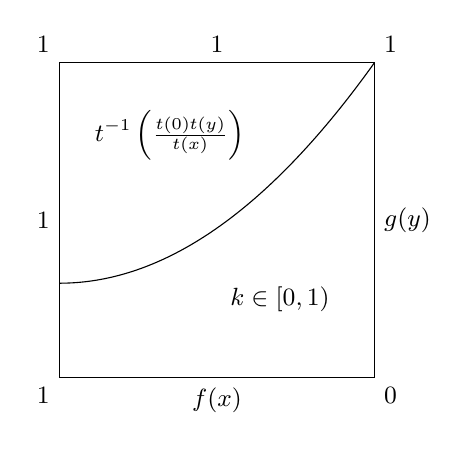
\begin{tikzpicture}[xscale=4, yscale=4]
		\draw (0,0) rectangle (1,1);
		\node [above right] at (1,1) {\small 1} ;
		\node [below right] at (1,0) {\small 0};
		\node [below left] at (0,0) {\small 1};
		\node [above left] at (0,1) {\small 1};
		\node [above] at (0.5,1) {\small 1};
		\node [left] at (0,0.5) {\small 1};
		\draw[domain=0:1,smooth,variable=\x,samples=200] plot (\x,{\x*\x*7/10+3/10});
		\node at (0.35,0.77) {\small $t^{-1} \left(\frac{t(0)t(y)}{t(x)}\right)$};
		\node at (0.7,0.25) {\small $k \in [0,1)$};
		\node [below] at (0.5,0) {\small $f(x)$};
		\node [right] at (1,0.5) {\small $g(y)$};
	\end{tikzpicture}
	\caption*{Case (ii)~~~~~~}
\end{subfigure}\\
\begin{subfigure}{.4\textwidth}
	\centering
	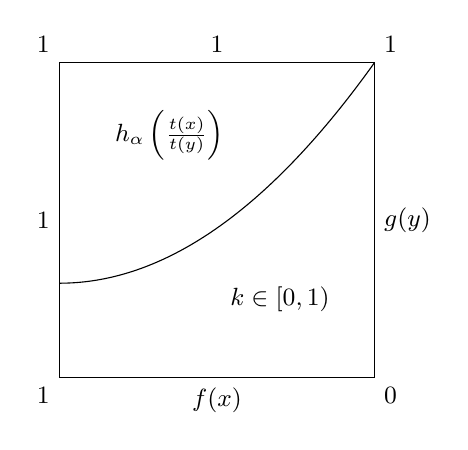
\begin{tikzpicture}[xscale=4, yscale=4]
		\draw (0,0) rectangle (1,1);
		\node [above right] at (1,1) {\small1} ;
		\node [below right] at (1,0) {\small0};
		\node [below left] at (0,0) {\small1};
		\node [above left] at (0,1) {\small1};
		\node [above] at (0.5,1) {\small1};
		\node [left] at (0,0.5) {\small1};
		\node at (0.35,0.77) {\small $h_{\alpha}\left(\frac{t(x)}{t(y)}\right)$};
		\draw[domain=0:1,smooth,variable=\x,samples=200] plot (\x,{\x*\x*7/10+3/10});
		\node at (0.7,0.25) {\small $k \in [0,1)$};
		\node [below] at (0.5,0) {\small $f(x)$};
		\node [right] at (1,0.5) {\small $g(y)$};
		%\node [below,rotate=30] at (0.35,0.60) {\scriptsize $y=t^{-1}(t(x)/\alpha)$};
	\end{tikzpicture}
	\caption*{Case (iii)~~~~~~}
\end{subfigure}%
\begin{subfigure}{.4\textwidth}
	\centering
	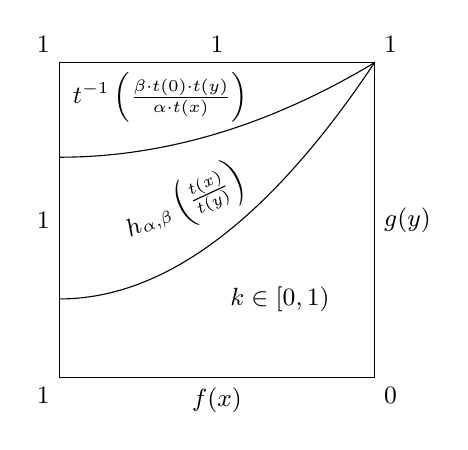
\begin{tikzpicture}[xscale=4, yscale=4]
		\draw (0,0) rectangle (1,1);
		\node [above right] at (1,1) {\small1} ;
		\node [below right] at (1,0) {\small0};
		\node [below left] at (0,0) {\small1};
		\node [above left] at (0,1) {\small1};
		\node [above] at (0.5,1) {\small1};
		\node [left] at (0,0.5) {\small1};
		\node at (0.32,0.89) {\small $t^{-1} \left(\frac{\beta \cdot t(0) \cdot t(y)}{\alpha \cdot t(x)}\right)$};
		\draw[domain=0:1,smooth,variable=\x,samples=200] plot (\x,{\x*\x*3/4+1/4});
		\draw[domain=0:1,smooth,variable=\x,samples=200] plot (\x,{\x*\x*3/10+7/10});
		\node at (0.7,0.25) {\small $k \in [0,1)$};
		\node [below] at (0.5,0) {\small $f(x)$};
		\node [right] at (1,0.5) {\small $g(y)$};
		%\node [right,rotate=15] at (0,0.6) {\tiny $y=t^{-1}(t(x)/\beta)$};
		%\node [right,rotate=18] at (0,0.15) {\tiny $y=t^{-1}(t(x)/\alpha)$};
		\node [rotate=25] at (0.4,0.55) {\small $h_{\alpha,\beta}\left(\frac{t(x)}{t(y)}\right)$};
	\end{tikzpicture}
	\caption*{Case (iv)~~~~~~}
\end{subfigure}
\caption[Schema of the structure of nilpotent $T$-power invariant implications that satisfy \EP.]{Schema of the structure of nilpotent $T$-power invariant implications that satisfy \EP defined in Proposition \ref{prop:nilpotent:(EP)}. In each case, the functions $f$ and $g$ can correspond to one of the cases in Lemma \ref{lem:nilpotent:(EP)f&g2}.}\label{figure:nilpotent:Structures(EP)}
\end{figure}

\begin{example}\label{example:nilpotent:(EP)}
Let us consider the Łukasiewicz t-norm \TLK, the additive generator $t(x)=1-x$ for all $x \in [0,1]$, $k=\frac{1}{4}$, $\alpha=2$, $\beta=4$ and the functions
$$
f_1(x)
=
\left\{ \begin{array}{ll}
	\frac{1}{4} &  \text{if }  x \leq \frac{1}{2}, \\[1pt]
	0 & \text{if } x>\frac{1}{2}, 
\end{array}
\right.
\quad
g_1(y)
=
\left\{ \begin{array}{ll}
	\frac{1}{4} &  \text{if }  y \geq \frac{1}{16}, \\[1pt]
	\sqrt{y} & \text{if } y<\frac{1}{16}. 
\end{array}
\right.	
$$
$$
f_2(x)=\frac{1}{4}, \quad \text{for all } x \in (0,1), \quad
g_2(y)
=
\left\{ \begin{array}{ll}
	\frac{1}{4} &  \text{if }  y \geq \frac{1}{8}, \\[1pt]
	0 & \text{if } y<\frac{1}{8}. 
\end{array}
\right.	
$$
$$f_3(x)=\frac{1}{4}(1-x^2), \quad x \in (0,1), \quad
g_3(y)
=
\left\{ \begin{array}{ll}
	\frac{1}{4} &  \text{if }  y \geq \frac{1}{4}, \\[1pt]
	y & \text{if } y<\frac{1}{4}. 
\end{array}
\right.	
$$
$$
\varphi_1(w)
=
\left\{ \begin{array}{ll}
	0 & \text{if } w=0, \\
	\frac{1}{4} &  \text{if }  w \leq 2, \\[1pt]
	1-\frac{1}{w} & \text{if } w>2, 
\end{array}
\right.
$$
$$
\varphi_2(w)
=
\left\{ \begin{array}{ll}
	0 & \text{if } w=0, \\
	\frac{1}{4} &  \text{if }  w \leq 2, \\[1pt]
	\frac{1}{2(1+e^{-5(w-2)})} & \text{if } w>2, 
\end{array}
\right.
\quad
\varphi_3(w)
=
\left\{ \begin{array}{ll}
	0 & \text{if } w=0, \\
	\frac{1}{4} &  \text{if }  w \leq 2, \\[1pt]
	\frac{1}{2(1+e^{-5(w-1.9)})} & \text{if } w>2, 
\end{array}
\right.	
$$
$$
\varphi_4(w)
=
\left\{ \begin{array}{ll}
	0 & \text{if } w=0, \\
	\frac{1}{4} &  \text{if }  w \leq 2, \\[1pt]
	\frac{3}{4(1+2^{3-w})} &  \text{if }  2<w<4, \\[1pt]
	1-\frac{2}{w}& \text{if } w>4, 
\end{array}
\right.
\quad
\varphi_5(w)
=
\left\{ \begin{array}{ll}
	0 & \text{if } w=0, \\
	\frac{1}{4} &  \text{if }  w \leq 2, \\[1pt]
	\frac{3}{4(1+1.5^{3-w})} &  \text{if }  2<w<4, \\[1pt]
	1-\frac{2}{w}& \text{if } w>4. 
\end{array}
\right.
$$
Then, $I_{\varphi_j,f_i,g_i}^{\TLK}$ is a nilpotent $\TLK$-power invariant implication for all $i \in \{1,2,3\}$ and $j \in \{1,2,3,4,5\}$. In Figure \ref{figure:nilpotent:(EP)} we can see the graphical representation of these functions. In that figure we can clearly see the behavior of the different cases in Proposition \ref{prop:nilpotent:(EP)}. Notice that depending on the choice of the different parameters and the functions $h_{\alpha}$ and $h_{\alpha,\beta}$ we can construct operators that are continuous in $(0,1)^2$ or not.

\begin{figure}[t]
	\centering
	\begin{subfigure}[t]{0.27\linewidth}\vspace{0pt}
		\centering
		\includegraphics[width=0.9\linewidth]{Example3-1.pdf}
		\caption{$I_{\varphi_1,f_1,g_1}^{\TLK}$}	
	\end{subfigure}%
	\begin{subfigure}[t]{0.27\linewidth}\vspace{0pt}
		\centering
		\includegraphics[width=0.9\linewidth]{Example3-2.pdf}
		\caption{$I_{\varphi_2,f_2,g_2}^{\TLK}$}
	\end{subfigure}%
	\begin{subfigure}[t]{0.27\linewidth}\vspace{0pt}
		\centering
		\includegraphics[width=0.91\linewidth]{Example3-3.pdf}
		\caption{$I_{\varphi_3,f_2,g_2}^{\TLK}$}		
	\end{subfigure}\\
	\begin{subfigure}[t]{0.27\linewidth}\vspace{0pt}
		\centering
		\includegraphics[width=0.9\linewidth]{Example3-4.pdf}
		\caption{$I_{\varphi_4,f_3,g_3}^{\TLK}$}	
	\end{subfigure}%
	\begin{subfigure}[t]{0.27\linewidth}\vspace{0pt}
		\centering
		\includegraphics[width=0.9\linewidth]{Example3-5.pdf}
		\caption{$I_{\varphi_5,f_3,g_3}^{\TLK}$}
	\end{subfigure}
	\caption[Plot of five nilpotent $\TLK$-power invariant implications that satisfy \EP.]{Plots of nilpotent $\TLK$-power invariant implications that satisfy \EP considered in Example \ref{example:nilpotent:(EP)}.}\label{figure:nilpotent:(EP)}
\end{figure}
\end{example}

\begin{remark}\label{remark:strict:(NPe)}
	It is interesting to notice that, in contrast with the analogous situation in the strict case (see Remark \ref{remark:(NPe)}), in the nilpotent case none of the solutions of \EP satisfy \NPe. Indeed, if \IT is a nilpotent $T$-power invariant implication satisfying \NPe then by Proposition \ref{prop:nilpotent:(NPe)}, \IT is given by Equation (\ref{eq:CandidateRU}). Then, since $\frac{t(e)}{t(0)}<1$ the constant region of $\varphi$ does not include (0,1) and this function does not correspond to any of the situations of Lemma \ref{lemma:nilpotent:(EP)varphi} and then it does not satisfy \EP.
\end{remark}

% LAW OF IMPORTATION %
Consecutively, we study the law of importation with respect to some t-norm. It is well known that \LI implies \EP, so our starting point are the fuzzy implication functions described in Proposition \ref{prop:nilpotent:(EP)}. We have seen that the solutions of \EP are significantly different in the strict and nilpotent cases so, one would expect the same situation when studying the law of importation. However, the next result proves that a nilpotent $T$-power invariant implication \IT that satisfies \LI must be constant in $(0,1)^2$. Then, by Lemma \ref{lem:nilpotent:InvariantVarphiConstant} we know that \IT is invariant with respect to the positive powers of any continuous t-norm, in particular, it is a strict $T^*$-power invariant implication for any strict t-norm $T^*$. Thus, the results on the law of importation in the strict case from Section \ref{subsection:additional_propertiesStrictTpower} are also valid for the nilpotent case and we do not list them here.
\pagebreak

\begin{lemma}\label{lem:nilpotent:(LI)}
Let \IT be a nilpotent $T$-power invariant implication that satisfies \LI with respect to a t-norm $T^*$, then there exists a $k \in [0,1]$ such that $\varphi(w)=k$ for all $w \in (0,+\infty)$.
\end{lemma}

\begin{proof}
It is well known that if \IT satisfies \LI with respect to a t-norm $T^*$ then it also fulfills \EP. Thus, $\varphi$ has one of the structures in Lemma \ref{lemma:nilpotent:(EP)varphi} and, in particular, $\varphi$ is constant to 1 in $(0,+\infty)$ or there exist $k \in [0,1)$ and $\alpha \in \left [ \frac{t(0)}{t(k)},1\right)$ such that $\varphi(w)=k$ for all $w \in (0,\alpha|$ and $\Ima g \subseteq [0,k]$. For this second case, let us consider $(y,z) \in (0,1)^2$ with $\IT(y,z) \in (0,1)$. Then,
$$k \leq \IT(y,z)=\IT(T^*(1,y),z)=\IT(1,\IT(y,z)) = g(\IT(y,z)) \leq k,$$
and $\IT(y,z)=k$. If $\IT(y,z) \in \{0,1\}$ for all $(y,z) \in (0,1)^2$ then by Lemma \ref{lemma:nilpotent:(EP)varphi} either $\varphi(w)=0$ for all $w \in [0,+\infty)$ or $\varphi(w)=1$ for all $w \in (0,+\infty]$. Thus, every situation leads to a $\varphi$  which is constant in $(0,+\infty)$.
\end{proof}

% ITERATIVE BOOLEAN RULE  %

Next, we consider the iterative boolean law. In this case, we can prove that $\varphi$ cannot be strictly increasing and, any interval in which $\varphi$ is constant to some $k \in (0,1)$ can be extended to $(0,+\infty)$.

\begin{lemma}\label{lem:nilpotent:(IB)}
Let \IT be a nilpotent $T$-power invariant implication that satisfies \IB. Then, the following properties hold:
\begin{enumerate}[label=(\roman*)]
	\item $g(y)=y$ for all $y \in \Ima g \setminus \{0,1\}$.
	\item $\varphi$ is not strictly increasing.
	\item If there exists a constant $k \in (0,1)$ and an interval $(a,b)$ with $a,b \in [0,+\infty)$ and $a<b$ such that $\varphi(w)=k$ for all $w \in (a,b)$ then $\varphi(w)=k$ for all $w \in (0,+\infty)$.
\end{enumerate}
\end{lemma}

\begin{proof}
\begin{enumerate}[label=(\roman*)]
	\item Consider $z \in \Ima g \setminus \{0,1\}$ then there exists $y \in (0,1)$ such that $g(y)=z$ and
	$$z=g(y)=\IT(1,y)=\IT(1,\IT(1,y))=\IT(1,z)=g(z).$$
	\item Assume that $\varphi$ is strictly increasing, then
	$$\varphi(1)=\IT(x,x)=\IT(x,\IT(x,x)) =\IT(x,\varphi(1)) = \varphi \left(\frac{t(x)}{t \circ \varphi(1)}\right),$$
	and $t(x)=t \circ \varphi(1)$ for all $x \in (0,1)$. Contradiction with the fact that $t$ is the additive generator of a nilpotent t-norm.
	\item First of all, we prove that $\varphi(w)=k$ for all $w \in \left(0,\frac{t(0)}{t(k)}\right)$ distinguishing between two cases:
	\begin{itemize}
		\item If $a \geq 1$ we consider $x_0 \in (0,1)$ and $y_0 \in \left( t^{-1} \left(\frac{t(x_0)}{a}\right), t^{-1} \left(\frac{t(x_0)}{b}\right)\right)$. In this case,
		$$k = \varphi \left(\frac{t(x_0)}{t(y_0)}\right) = \IT(x_0,y_0) = \IT(x_0,\IT(x_0,y_0)) = \IT(x_0,k) = \varphi \left(\frac{t(x_0)}{t(k)}\right).$$
		Thus, $\varphi(w)=k$ for all $w \in \left(0,\frac{t(0)}{t(k)}\right)$.
		\item If $a < 1$ then there exists an $n_0 \in \NN$ with $\left( \frac{t(0)}{t(k)} \right)^{n_0-1}a<1$ and $\left( \frac{t(0)}{t(k)} \right)^{n_0}a \geq 1$. We prove by induction on $n \in \{1,\dots,n_0\}$ that $\varphi(w)=k$ for all $w \in \left(0,\left(\frac{t(0)}{t(k)}\right)^{n_0}a\right)$.
		\begin{itemize}
			\item If $n=1$ we consider $x_0 > t^{-1}(a t(0))$ and $y_0 \in \left( t^{-1} \left(\frac{t(x_0)}{a}\right), t^{-1} \left(\frac{t(x_0)}{b}\right)\right)$. Then,
			\begin{eqnarray*}
			k &=& \varphi \left(\frac{t(x_0)}{t(y_0)}\right) = \IT(x_0,y_0) = \IT(x_0,\IT(x_0,y_0))= \IT(x_0,k) \\
			&=& \varphi \left(\frac{t(x_0)}{t(k)}\right),
			\end{eqnarray*}
			and $\varphi(w)=k$ for all $w \in \left(0,\frac{t(0)}{t(k)}a\right)$.
			\item We assume that $\varphi(w)=k$ for all $w \in \left(0,\left(\frac{t(0)}{t(k)}\right)^{n-1}a\right)$. Let us choose $x_0 > t^{-1} \left(a \frac{t(0)^n}{t(k)^{n-1}}\right)$ and $y_0 < t^{-1} \left(\frac{t(x_0)}{a} \left(\frac{t(k)}{t(0)}\right)^{n-1}\right)$. Then,
			\begin{eqnarray*}
			k &=& \varphi \left(\frac{t(x_0)}{t(y_0)}\right) = \IT(x_0,y_0) = \IT(x_0,\IT(x_0,y_0))= \IT(x_0,k) \\
			&=& \varphi \left(\frac{t(x_0)}{t(k)}\right),
			\end{eqnarray*}
			and $\varphi(w)=k$ for all $w \in \left(0,\left(\frac{t(0)}{t(k)}\right)^n a\right)$.
		\end{itemize}
		Finally, let us consider $x_0 \in (0,1)$ and $y_0 < t^{-1} \left(\frac{t(x_0)t(k)^{n_0}}{at(0)^{n_0}}\right)$. Then,
		$$k = \varphi \left(\frac{t(x_0)}{t(y_0)}\right) = \IT(x_0,y_0) = \IT(x_0,\IT(x_0,y_0))= \IT(x_0,k) = \varphi \left(\frac{t(x_0)}{t(k)}\right),$$
		and  $\varphi(w)=k$ for al $w \in \left(0,\frac{t(0)}{t(k)}\right)$.			
	\end{itemize}
	On the other hand, assume that there exists a $w_0 \in \left[ \frac{t(0)}{t(k)},+\infty\right)$ with $\varphi(w_0)>k$. Then, $t \circ \varphi (w_0) < t(k) \Rightarrow \frac{t \circ \varphi(w_0)}{t(k)} < 1 \Rightarrow \frac{t \circ \varphi(w_0)t(0)}{t(k)}<t(0)$. Let us choose $x_0 \in \left(t^{-1} \left(\frac{t(0) t \circ \varphi(w_0)}{t(k)}\right),1\right)$, since  $\frac{t(x_0)}{t(0)}<1<\frac{t(0)}{t(k)} \leq w_0$ there exists a $y_0 \in (0,1)$ such that $\frac{t(x_0)}{t(y_0)}=w_0$. In this case,
	\begin{eqnarray*}
	\varphi(w_0) &=& \varphi\left(\frac{t(x_0)}{t(y_0)}\right) = \IT(x_0,y_0) = \IT(x_0,\IT(x_0,y_0)) =\IT(x_0,\varphi(w_0)) \\
	&=& \varphi \left(\frac{t(x_0)}{t \circ \varphi(w_0)}\right)=k,
	\end{eqnarray*}
	which is a contradiction. Then $\varphi$ is constant to $k$ in $(0,+\infty)$.
\end{enumerate}
\end{proof}

The next result characterizes the nilpotent $T$-power invariant implications that satisfy \IB.

\begin{proposition}\label{prop:nilpotent:(IB)}
Let \IT be a nilpotent $T$-power invariant implication. Then \IT satisfies \IB if and only if one of the following conditions hold:
\begin{enumerate}[label=(\roman*)]
	\item $\varphi(w)=0$ for all $w \in (0,+\infty)$ and $f(x)=g(y)=0$ for all $x,y \in (0,1)$.
	\item 						$$
	\varphi(w)
	=
	\left\{ \begin{array}{ll}
		0 &   \text{if }   w \in (0,b|, \\
		1 & \text{if } w \in (0,+\infty] \setminus (0,b|,
	\end{array}
	\right.
	$$
	where $b \in (0,1)$, $ \Ima f \subseteq \{0,1\}$, $f(x)=0$ for all $x \in (0,1)$ such that $\frac{t(x)}{t(0)} \in (0,b|$ and $g(y)=0$ for all $y \in (0,1)$.
	\item Let $k \in (0,1]$, then $\varphi(w)=k$ for all $w \in (0,+\infty)$, $\Ima f  \subseteq \{0,k\}$, $\Ima g \subseteq [0,k]$ and $g(y)=y$ for all $y \in \Ima g \setminus \{0,1\}$.
\end{enumerate}
\end{proposition}

\begin{proof}
\begin{itemize}
	\item[($\Rightarrow$)] By (ii)-Lemma \ref{lem:nilpotent:(IB)} we know that $\varphi$ is not strictly increasing, i.e., it is constant in some interval. We distinguish between four cases:
	\begin{enumerate}[label=\alph*)]
		\item $\varphi(w)=0$ for all $w \in (0,+\infty)$ then by Lemma \ref{lem:nilpot:monotonicity_condition:necessicity} we have that $f(x)=g(y)=0$ for all $x,y \in (0,1)$ and we are in Case (i).
		\item If there exists a $b \in (0,+\infty)$ such that $\varphi(w)=0$ if and only if $w \in (0,b|$, then by Lemma \ref{lem:nilpot:monotonicity_condition:necessicity}, $g(y)=0$ for all $y \in (0,1)$ and by Condition (\ref{eq:def:nilpot:TPowerInv:MonotonicityCond}) we get that $f(x)=0$ when $\frac{t(x)}{t(0)} \in (0,b|$ for all $x \in (0,1)$. Let us consider $\varphi(w_0) \in (0,1)$ with $w_0 \in (0,+\infty) \setminus (0,b|$, if we choose $x_0>t^{-1} (\min \{t(0),bt \circ \varphi(w_0)\})$ then $\frac{t(x_0)}{t(0)}< \frac{b t \circ \varphi(w_0)}{t(0)}<b$ and there exists a $y_0 \in (0,1)$ such that $\frac{t(x_0)}{t(y_0)}=w_0$. Thus,
		\begin{eqnarray*}
			\varphi(w_0)&=&\varphi \left(\frac{t(x_0)}{t(y_0)}\right) = \IT(x_0,y_0) = \IT(x_0,\IT(x_0,y_0)) = \IT(x_0,\varphi(w_0)) \\
			&=& \varphi \left(\frac{t(x_0)}{t \circ \varphi(w_0)}\right)=0,
		\end{eqnarray*}
		and we obtain a contradiction with the fact that \IT satisfies \IB. Then $\Ima \varphi \subseteq \{0,1\}$ and we are in Case (ii).
		\item If $\varphi(w)=k$ with $k \in (0,1)$ for all $w \in (a,b)$ with $a,b \in [0,+\infty)$ and $a<b$, by (iii)-Lemma \ref{lem:nilpotent:(IB)} we have that $\varphi(w)=k$ for all $w \in (0,+\infty)$.
		\item Consider the situation where there exists $a \in (0,+\infty)$ such that $\varphi(w)=1$ for all $w \in |a,+\infty]$. If $\varphi(w_0)=0$ for some $w_0 \in (0,a]$ we are in the same situation as in b), then we assume that $\varphi(w) \in (0,1]$ for all $w \in (0,+\infty]$. On the other hand, if $\varphi$ is constant to some $k \in (0,1)$ in some interval, by c) we would obtain a contradiction, then $\varphi$ must be strictly increasing when it is not constant to 1. Let us assume that there exists a $w_0 \in (0,a]$ with $\varphi(w_0) \in (0,1)$, then if we choose $x_0 > t^{-1}(\min \{t(0), w_0 t \circ \varphi(w_0)\})$ we have $\frac{t(x_0)}{t(0)} < \frac{w_0 t \circ \varphi(w_0)}{t(0)} < w_0$ and there exists $y_0 \in (0,1)$ such that $\frac{t(x_0)}{t(y_0)}=w_0$. Then,
		\begin{eqnarray*}
		\varphi(w_0) &=& \varphi \left(\frac{t(x_0)}{t(y_0)}\right) = \IT(x_0,y_0) = \IT(x_0,\IT(x_0,y_0)) \\
		&=& \IT(x_0,\varphi(w_0)) 
		= \varphi \left(\frac{t(x_0)}{t \circ \varphi(w_0)}\right).
		\end{eqnarray*}
		Since $\varphi$ is strictly increasing, we have $t(x_0)=w_0 t \circ \varphi(w_0)$. Contradiction with the fact that $x_0$ was selected to satisfy $t(x_0)<w_0t\circ \varphi(w_0)$. Then, $\varphi(w)=1$ for all $w \in (0,+\infty)$.	
	\end{enumerate}
	The points b) and c) correspond to situations where $\varphi(w)=k$ for all $w \in (0,+\infty)$ with $k \in (0,1]$. By Lemma \ref{lem:nilpot:monotonicity_condition:necessicity} we have $\Ima f \subseteq [0,k]$ and $\Ima g \subseteq [0,k]$ and by (i)-Lemma \ref{lem:nilpotent:(IB)} we know that $g(y)=y$ for all $y \in \Ima g \setminus \{0,1\}$. Let us assume that there exists an $x_0 \in (0,1)$ with $f(x_0) \in (0,k)$, then
	$$f(x_0) = \IT(x_0,0) = \IT(x_0,\IT(x_0,0)) = \IT(x_0,f(x_0))=k,$$
	which is a contradiction. Then, this situation corresponds to Case (iii).  
	\item[($\Leftarrow$)] Cases (i) and (iii) do not depend on the additive generator of the t-norm $T$, so these solutions were already considered in Proposition \ref{prop:strict:(IB)}. Then, we only check Case (ii). On the one hand,
	$$
	\IT(x,y)
	=
	\left\{ \begin{array}{ll}
		0 &   \text{if }   x=1 \text{ and } y \in (0,1), \\
		0 &   \text{if }   x,y \in (0,1) \text{ and } \frac{t(x)}{t(y)} \in (0,b|, \\
		f(x) &   \text{if }   x \in (0,1) \text{ and } y=0, \\
		1 & \text{otherwise}.
	\end{array}
	\right.
	$$
	On the other hand,
	\begin{eqnarray*}
		\IT(x,\IT(x,y))
		&=&
		\left\{ \begin{array}{ll}
			\IT(1,0) &   \text{if }   x=1 \text{ and } y \in (0,1), \\[1pt]
			\IT(x,0) &   \text{if }   x,y \in (0,1) \text{ and } \frac{t(x)}{t(y)} \in (0,b|, \\[3pt]
			\IT(x,f(x)) &   \text{if }   x \in (0,1) \text{ and } y=0, \\[3pt]
			\IT(x,1) & \text{otherwise},
		\end{array}
		\right. \\
		&=&
		\left\{ \begin{array}{ll}
			0 &   \text{if }   x=1 \text{ and } y \in (0,1), \\
			0 &   \text{if }   x,y \in (0,1) \text{ and } \frac{t(x)}{t(y)} \in (0,b|, \\
			\IT(x,0) &   \text{if }   x \in (0,1), y=0 \text{ and } f(x)=0, \\[3pt]
			\IT(x,1) &   \text{if }   x \in (0,1), y=0 \text{ and } f(x)=1, \\
			1 & \text{otherwise}, 
		\end{array} \right.  \\
		&=& \IT(x,y). 
	\end{eqnarray*}
	
\end{itemize}
\end{proof}

In this case, the solutions are very similar to the strict case (see Proposition \ref{prop:strict:(IB)}). However, notice that in Case (ii) the expression of the corresponding nilpotent $T$-power invariant depends on the generator $t$, so it is not the same situation of Case (i) in Proposition \ref{prop:strict:(IB)} and the strict and nilpotent cases are not equivalent.

Finally, we study the $T$-conditionality with respect to the same t-norm considered in the invariance property. For this property we obtain very different results than in the strict case (see Proposition \ref{prop:strict:(TC)}) since we obtain solutions that are not necessary $0$ whenever $x>y$. Indeed, a nilpotent $T$-power invariant implications satisfies \TC with respect to $T$ if and only if $\varphi$ and $f$ satisfy a certain inequality involving an additive generator of $T$.
\begin{proposition}\label{Nilpotent:(TC)}
	Let \IT be a nilpotent $T$-power invariant implication and $t$ an additive generator of~$T$. Then \IT satisfies  \TC with respect to $T$ if and only if $\varphi(w) \leq t^{-1} \left(t(0)(1-w)\right)$ for all $w \in [0,1)$, $f(x) \leq t^{-1}(t(0)-t(x))$ for all $x \in (0,1)$ and $g(y)=0$ for all $y \in (0,1)$.
\end{proposition}
\begin{proof}
	\begin{itemize}
		\item[$(\Rightarrow)$] Let \IT be a nilpotent $T$-power invariant implication that satisfies \TC with respect to $T$. Let us assume that there exists a $\tilde{w} \in (0,1)$ such that $\varphi(\tilde{w})>t^{-1}(t(0)(1-\tilde{w}))$, therefore, there exists a $\tilde{y} \in (0,1)$ such that $\varphi(\tilde{w})>t^{-1}(t(\tilde{y})(1-\tilde{w}))>t^{-1}(t(0)(1-\tilde{w}))$. Since $\left\{\frac{t(x)}{t(\tilde{y})} \mid x \in (0,1)\right\} = \left(0,\frac{t(0)}{t(\tilde{y})}\right)$ there exists an $\tilde{x} \in (\tilde{y},1)$ such that $\tilde{w}=\frac{t(\tilde{x})}{t(\tilde{y})}$. In this case,
		\begin{eqnarray*}
			\varphi(\tilde{w})>t^{-1}(t(\tilde{y})(1-\tilde{w})) & \Rightarrow &  \varphi\left(\frac{t(\tilde{x})}{t(\tilde{y})}\right)>t^{-1}\left(t\left(\tilde{y}\right)\left(1-\frac{t(\tilde{x})}{t(\tilde{y})}\right)\right)\\
			& \Rightarrow &  \varphi\left(\frac{t(\tilde{x})}{t(\tilde{y})}\right)>t^{-1}\left(t(\tilde{y})-t(\tilde{x})\right) \\
			& \Rightarrow &  t(\tilde{x}) + t\left(\varphi\left(\frac{t(\tilde{x})}{t(\tilde{y})}\right)\right)<t(\tilde{y})<t(0) \\
			& \Rightarrow &  t^{-1}\left(t(\tilde{x}) + t\left(\varphi\left(\frac{t(\tilde{x})}{t(\tilde{y})}\right)\right)\right) > \tilde{y} \\
			& \Rightarrow &  T(\tilde{x},I(\tilde{x},\tilde{y})) > \tilde{y},
		\end{eqnarray*}
		and we obtain a contradiction with the fact that \IT and $T$ satisfy \TC. On the other hand, let us assume that there exists an $\tilde{x} \in (0,1)$ such that $f(\tilde{x}) > t^{-1}(t(0)-t(\tilde{x}))$. Then, there exists a $\tilde{y} \in (0,1)$ such that $f(\tilde{x}) > t^{-1}(t(\tilde{y})-t(\tilde{x})) > t^{-1}(t(0)-t(\tilde{x}))$ and we have
		\begin{eqnarray*}
			f(\tilde{x}) > t^{-1}(t(\tilde{y})-t(\tilde{x}))  & \Rightarrow &  t(\tilde{x})+t(f(\tilde{x})) < t(\tilde{y})<t(0)\\
			& \Rightarrow &  t^{-1}\left(t(\tilde{x})+t(f(\tilde{x}))\right) > \tilde{y}\\
			& \Rightarrow &  T(\tilde{x},I(\tilde{x},0)) > \tilde{y} >0,
		\end{eqnarray*}
		and we obtain a contradiction with the fact that \IT and $T$ satisfy \TC. Finally, since $\displaystyle \lim_{w \to 0^+} \varphi(w) \leq \lim_{w \to 0^+} t^{-1} \left(t(0)(1-w)\right) = 0$ by Lemma \ref{lem:nilpot:monotonicity_condition:necessicity} we obtain that $g(y)=0$ for all $ y \in (0,1)$.
		\item[$(\Leftarrow)$] Let $x,y \in [0,1]$ with $x>y$. We distinguish between different cases:
		\begin{itemize}
			\item If $x=1$ and $y \in [0,1)$ then
			$$T(x,I(x,y))=T(1,I(1,y))=I(1,y)=\left\{ \begin{array}{ll}
				g(y) &   \text{if }   y \in (0,1), \\
				0 &  \text{if }   y=0,
			\end{array}
			\right.
			=0 \leq y.$$
			\item If $y=0$ and $x \in (0,1)$ then
			\begin{eqnarray*}
				I(x,0)=f(x) \leq t^{-1}(t(0)-t(x)) & \Rightarrow & t(x)+t(I(x,0)) \geq t(0)\\
				&\Rightarrow& t^{(-1)}(t(x)+t(I(x,0)))=0\\
				&\Rightarrow& T(x,I(x,0))=0=y.
			\end{eqnarray*}
			\item If $0<y<x<1$ then
			$$\varphi \left(\frac{t(x)}{t(y)}\right) \leq t^{-1}\left(t(0)\left(1-\frac{t(x)}{t(y)}\right)\right) \leq t^{-1}\left(t(y)\left(1-\frac{t(x)}{t(y)}\right)\right) = t^{-1}(t(y)-t(x)),$$
			$$t(x) + t \left(\varphi \left(\frac{t(x)}{t(y)}\right)\right) \geq t(y),$$
			and we distinguish between two cases.
			\begin{itemize}
				\item If $t(x) + t \left(\varphi \left(\frac{t(x)}{t(y)}\right)\right) \geq t(0)$ then
				$$T(x,I(x,y))= t^{(-1)}\left(t(x) + t \left(\varphi \left(\frac{t(x)}{t(y)}\right)\right)\right) = 0 \leq y.$$
				\item $t(x) + t \left(\varphi \left(\frac{t(x)}{t(y)}\right)\right) < t(0)$ then 
				$$T(x,I(x,y))=t^{-1}\left(t(x) + t \left(\varphi \left(\frac{t(x)}{t(y)}\right)\right)\right) \leq y.$$
			\end{itemize}
		\end{itemize}
	\end{itemize}
\end{proof}
Proposition \ref{Nilpotent:(TC)} discloses an important breakthrough. It is known that the $T$-conditionality is recommended for doing any inference with the generalized modus ponens when a fuzzy implication function is used as the generalization of the classical conditional to fuzzy logic. Therefore, it is a property which is required for many applications. Besides, we have already motivated the importance of the $T$-power invariance when fuzzy hedges modeled by powers of continuous t-norms are used. Proposition \ref{Nilpotent:(TC)} ensures the existence of many fuzzy implication functions satisfying \PIT and \TC with respect to a nilpotent t-norm $T$. From this fact, we can affirm that this family is very appealing for many practical applications. Not only that, the conditions in Proposition \ref{Nilpotent:(TC)} are general enough to allow some flexibility in the structure of the operator. Indeed, for instance if we consider $\varphi(w)= \alpha t^{-1}(t(0)(1-w))$ for all $w \in [0,1)$ with $\alpha \in (0,1)$ we have the freedom of choosing the values of the function $\varphi$ in  $w \in [1,+\infty]$ (as long as we respect the conditions in Definition \ref{def:nilpot:TPowerInv}). For instance, in Example \ref{example:ITLKalpha} we have considered $\varphi(w)=\frac{(1+\alpha)w+\alpha-1}{(1+\alpha)w-\alpha+1}$ for all  $w \in [1,+\infty]$ to define a family of fuzzy implication functions that is a particular case of those described in Proposition \ref{Nilpotent:(TC)}. It is curious how the invariance property together with other well-known properties like \NP or \LI is so strong that imposes that the corresponding nilpotent $T$-power invariant implication must be constant in $(0,1)^2$ and with other properties like \TC or \EP is flexible enough to allow us to select arbitrarily the expression of the operator in a subregion of $[0,1]^2$.
\begin{example}\label{example:ITLKalpha}
	Let $T$ be a nilpotent t-norm and $t$ an additive generator of $T$. Let us consider $\alpha \in (0,1]$ and $\varphi:[0,+\infty] \to [0,1]$, $g:(0,1) \to [0,1]$, $f: (0,1) \to [0,1]$ given by
	$$f(x)=g(y)=0, \quad \text{ for all } x,y \in (0,1),$$
	$$\varphi(w) 
	=
	\left\{ \begin{array}{ll}
		\alpha t^{-1}(t(0)(1-w)) &   \text{if }   w \in [0,1), \\
		\frac{(1+\alpha)w+\alpha-1}{(1+\alpha)w-\alpha+1} & \text{if } w \in [1,+\infty].
	\end{array}
	\right.
	$$
	Then, according to Proposition \ref{Nilpotent:(TC)} the corresponding nilpotent $T$-power invariant implication satisfies \TC with respect to $T$ for all $\alpha \in (0,1]$. Let us denote this family of functions as $I_{\alpha}^T : [0,1]^2 \to [0,1]$, their expression is
	\begin{equation}\label{eq:Family(TC)(IT)}
		I_{\alpha}^T(x,y) =\left\{ \begin{array}{ll}
			0 &   \text{if }   (x \in (0,1] \text{ and } y=0) \text{ or } (x = 1 \text{ and } y\in (0,1)), \\
			\alpha t^{-1}\left(t(0) \left(1-\frac{t(x)}{t(y)}\right)\right) & \text{if } 0<y<x<1, \\
			\frac{(1+\alpha)t(x)-(1-\alpha)t(y)}{(1+\alpha)t(x)+(1-\alpha)t(y)} & \text{if } 0<x\leq y<1, \\
			1 & \text{if } (x=0 \text{ and } y \in [0,1]) \text{ or } (x \in (0,1] \text{ and } y=1),
		\end{array}
		\right.
	\end{equation}
	for all $\alpha \in (0,1]$. In Figure \ref{fig:IalphaT} we can find a sketch of the structure of this subfamily of nilpotent $T$-power invariant implications. In particular, if we select $\alpha=1$ we have a family that also satisfies \IP and \OP  (see Proposition \ref{prop:nilpotent:(OP)n(IP)}).
	\begin{figure}[htp!]
		\centering
		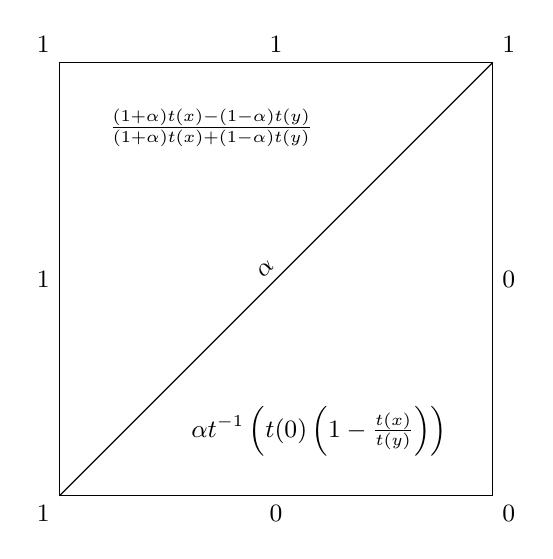
\begin{tikzpicture}[xscale=5.5, yscale=5.5]
			\draw (0,0) rectangle (1,1);
			\node [above right] at (1,1) {\small 1} ;
			\node [below right] at (1,0) {\small 0};
			\node [below left] at (0,0) {\small 1};
			\node [above left] at (0,1) {\small 1};
			\node [above] at (0.5,1) {\small 1};
			\node [left] at (0,0.5) {\small 1};
			\node [above,rotate=45] at (0.5,0.5) {\small $\alpha$};
			\draw (0,0) -- (1,1);
			\node at (0.35,0.85) {\small $\frac{(1+\alpha)t(x)-(1-\alpha)t(y)}{(1+\alpha)t(x)+(1-\alpha)t(y)}$};
			\node at (0.6,0.15) {\small $\alpha t^{-1}\left(t(0) \left(1-\frac{t(x)}{t(y)}\right)\right)$};
			\node [below] at (0.5,0) {\small $0$};
			\node [right] at (1,0.5) {\small $0$};
		\end{tikzpicture}
		\caption{Schema of the structure of $I_{\alpha}^T$.}\label{fig:IalphaT}
	\end{figure}
	\begin{figure}[t!]
		\centering
		\begin{subfigure}[t]{0.35\linewidth}\vspace{0pt}
			\centering
			\includegraphics[width=0.9\linewidth]{ITalpha0.25.pdf}
			\caption{$I_{\alpha=0.25}^{\TLK}$}	
		\end{subfigure}%
		\begin{subfigure}[t]{0.35\linewidth}\vspace{0pt}
			\centering
			\includegraphics[width=0.9\linewidth]{ITalpha0.5.pdf}
			\caption{$I_{\alpha=0.5}^{\TLK}$}
		\end{subfigure}\\ \vspace{0.5cm}
		\begin{subfigure}[t]{0.35\linewidth}\vspace{0pt}
			\centering
			\includegraphics[width=0.91\linewidth]{ITalpha0.75.pdf}
			\caption{$I_{\alpha=0.75}^{\TLK}$}		
		\end{subfigure}%
		\begin{subfigure}[t]{0.35\linewidth}\vspace{0pt}
			\centering
			\includegraphics[width=0.9\linewidth]{ITalpha1.pdf}
			\caption{$I_{\alpha=1}^{\TLK}$}	
		\end{subfigure}
		\caption{Plot of the fuzzy implication function $I^T_{\alpha}$ where $T=\TLK$ for different values of the parameter $\alpha$.}\label{figure:ITLKalpha}
	\end{figure}
\end{example}
\begin{remark}
	The reader might have noticed that, unlike the case of the study of \LI, for \TC we have not considered the problem for a t-norm $T^*$ that might be different from the one used when imposing \PIT. We have decided not to study this case because of the complexity attached. It is rather straightforward to notice that \TC is more complex to study than \LI in this case because the first one is an inequality. However, some results in the particular case of $T$-power based implications can be found in \cite{Li2022,Peng2022}.
\end{remark}

\subsection{Summary}
To end this section we provide a summary in Table  \ref{table:summaryTpowerinvadditionalprop} of all the additional properties studied for the family of $T$-power invariant implication where $T$ is a continuous Archimedean t-norm and also of $T$-power based implications as a particular case. In this table, we can compare two perspectives: to study a family that satisfies a certain property and to study a family characterized by the fact that they fulfill a certain property. It is intuitive to think that the second perspective is much more stronger and provides more information. Indeed, in this chapter we have empirically proved this fact. In Table  \ref{table:summaryTpowerinvadditionalprop} we can see that although the power based implications satisfy the invariance property, they do not satisfy many of the other additional properties of fuzzy implication functions. On the other hand, studying the families characterized by the fact that they fulfill \PIT with respect to a certain Archimedean t-norm we have proved that there is always a choice satisfying also another additional property (except the continuity). Furthermore, as argued along the section, in this study we have obtain many interesting fuzzy implication functions which behave very differently from power-based implications. \enlargethispage{12pt}
\begin{table}[!t]
	\begin{adjustbox}{max width=\textwidth}
	\begin{tabular}{c|cc|cc|}
		\cline{2-5}
		\multicolumn{1}{l|}{}                  & \multicolumn{2}{l|}{\bf $T$-power based implications} & \multicolumn{2}{l|}{\bf $T$-power invariant implications} \\ \cline{2-5} 
		& \multicolumn{1}{c|}{\bf $T$ strict}   & \bf $T$ nilpotent   & \multicolumn{1}{c|}{\bf $T$ strict}     & \bf $T$ nilpotent     \\ \hline
		\multicolumn{1}{|c|}{\bf Continuity}       & \multicolumn{1}{c|}{\xmark}           &   \multicolumn{1}{c|}{\xmark}            & \multicolumn{1}{c|}{\begin{tabular}[c]{@{}c@{}c@{}}\xmark\\ Proposition \ref{prop:strict:continuity} \\ Corollary \ref{cor:strict:discontinuous} \end{tabular}}            &        \begin{tabular}[c]{@{}c@{}c@{}}\xmark\\ Proposition \ref{prop:nilpotent:continuity} \\ Corollary \ref{cor:nilpotent:discontinuous} \end{tabular}         \\ \hline
		\multicolumn{1}{|c|}{\bf Natural Negation}   & \multicolumn{1}{c|}{\NDOne}           &      \multicolumn{1}{c|}{$N_{I^T}(x)=\frac{t(x)}{t(0)}$}         & \multicolumn{1}{c|}{Corollary \ref{cor:strict:natural_negation}}             &        \multicolumn{1}{c|}{Corollary \ref{cor:nilpotent:natural_negation}}          \\ \hline
		\multicolumn{1}{|c|}{\bf Trivial 1-region} & \multicolumn{1}{c|}{\xmark}            &  \multicolumn{1}{c|}{\xmark}              & \multicolumn{1}{c|}{Proposition \ref{prop:strict:1-region}}             &   \multicolumn{1}{c|}{Proposition \ref{prop:nilpotent:1-region}}               \\ \hline
		\multicolumn{1}{|c|}{\CB}             & \multicolumn{1}{c|}{\xmark}            &    \multicolumn{1}{c|}{\xmark}            & \multicolumn{1}{c|}{\begin{tabular}[c]{@{}c@{}} Proposition \ref{prop:strict:(CB)} \\ Constant in $(0,1)^2$ \end{tabular}}            &       \multicolumn{1}{c|}{\begin{tabular}[c]{@{}c@{}} Proposition \ref{prop:nilpot:(CB)} \\ Constant in $(0,1)^2$ \end{tabular}}          \\ \hline
		\multicolumn{1}{|c|}{\NP}             & \multicolumn{1}{c|}{\xmark}            &    \multicolumn{1}{c|}{\xmark}            & \multicolumn{1}{c|}{\begin{tabular}[c]{@{}c@{}} Proposition \ref{prop:strict:(NP)} \\ Constant in $(0,1)^2$ \end{tabular}}            &       \multicolumn{1}{c|}{\begin{tabular}[c]{@{}c@{}} Proposition \ref{prop:nilpotent:(NP)} \\ Constant in $(0,1)^2$ \end{tabular}}           \\ \hline
		\multicolumn{1}{|c|}{\NPe}            & \multicolumn{1}{c|}{\xmark}           &     \multicolumn{1}{c|}{\xmark}           & \multicolumn{1}{c|}{Proposition \ref{prop:strict:(NPe)}}             &     \multicolumn{1}{c|}{Proposition \ref{prop:nilpotent:(NPe)}}             \\ \hline
		\multicolumn{1}{|c|}{\IP}             & \multicolumn{1}{c|}{\cmark}            &       \multicolumn{1}{c|}{\cmark}         & \multicolumn{1}{c|}{Proposition \ref{prop:strict:(IP)n(OP)}}             &      \multicolumn{1}{c|}{Proposition \ref{prop:nilpotent:(OP)n(IP)}}            \\ \hline
		\multicolumn{1}{|c|}{\OP}             & \multicolumn{1}{c|}{\cmark}           &    \multicolumn{1}{c|}{\cmark}            & \multicolumn{1}{c|}{Proposition \ref{prop:strict:(IP)n(OP)}}             &     \multicolumn{1}{c|}{Proposition \ref{prop:nilpotent:(OP)n(IP)}}             \\ \hline
		\multicolumn{1}{|c|}{\EP}             & \multicolumn{1}{c|}{\xmark}            &     \multicolumn{1}{c|}{\xmark}           & \multicolumn{1}{c|}{Proposition \ref{prop:strict:(EP)}}             &      \multicolumn{1}{c|}{Proposition \ref{prop:nilpotent:(EP)}}           \\ \hline
		\multicolumn{1}{|c|}{\bf \LI with $T^*$}             & \multicolumn{1}{c|}{\xmark}           &        \multicolumn{1}{c|}{\xmark}        & \multicolumn{1}{c|}{\begin{tabular}[c]{@{}c@{}} Proposition \ref{prop:strict:(LI)} \\ Constant in $(0,1)^2$ \end{tabular}}             &     \multicolumn{1}{c|}{\begin{tabular}[c]{@{}c@{}c@{}} Lemma \ref{lem:nilpotent:(LI)} \\ Proposition \ref{prop:strict:(LI)} \\ Constant in $(0,1)^2$ \end{tabular}}             \\ \hline
		\multicolumn{1}{|c|}{\bf (IB)}             &\multicolumn{1}{c|}{\xmark}            & \multicolumn{1}{c|}{\xmark}               & \multicolumn{1}{c|}{Proposition \ref{prop:strict:(IB)}}             &          \multicolumn{1}{c|}{Proposition \ref{prop:nilpotent:(IB)}}         \\ \hline
		\multicolumn{1}{|c|}{\bf \TC with $T$}      & \multicolumn{1}{c|}{\xmark}           &  \multicolumn{1}{c|}{\cite[Theorem 3.2]{Peng2022}}             & \multicolumn{1}{c|}{Proposition \ref{prop:strict:(TC)}}             &       \multicolumn{1}{c|}{Proposition \ref{Nilpotent:(TC)}}            \\ \hline
	\end{tabular}
	\end{adjustbox}
\caption[Summary of the properties fulfilled by $T$-power based implications and by $T$-power invariant implications where $T$ is a continuous Archimedean t-norm.]{Summary of the properties fulfilled by $T$-power based implications and by $T$-power invariant implications where $T$ is a continuous Archimedean t-norm. The results involving $T$-power based implications are either available in \cite{Massanet2017} or they have been deduced from the results of this section.}\label{table:summaryTpowerinvadditionalprop}
\end{table}
\section{Intersections}\label{section:intersectionsTpower}

In this section, we investigate the intersections between the families of strict and nilpotent $T$-power invariant implications and ten of the main families of fuzzy implication functions. This step is very important when studying a new family of fuzzy implication functions since it proves that the newly introduced family is significantly different from other  families in the literature. Moreover, in our particular case, this study has an added value, since studying the intersection between the family of strict/nilpotent $T$-power invariant implications and another family is equivalent to characterize all the fuzzy implication functions of this family which are invariant with respect to $T$-powers of a certain strict/nilpotent t-norm.

First of all, we study the intersection between the studied families, i.e., strict and nilpotent $T$-power invariant implications. In Lemma \ref{lem:nilpotent:InvariantVarphiConstant} we have already proved that if $\varphi$ is constant, the dependence on the generator disappears, and a nilpotent $T$-power invariant implication is, in fact, invariant with respect to the positive powers of any continuous t-norm, so it is also a strict $T^*$-power invariant implication for any strict t-norm $T^*$. However, the following result completely characterizes the intersection between the two families, that will be denoted by:
\begin{eqnarray*}
	\mathbb{I}^{\infty}_{Inv} &~-~& \text{the family of all fuzzy implication functions which are invariant} \\
	&~~~& \text{with respect to the positive powers of some strict t-norm}; \\
	\mathbb{I}^{\aleph}_{Inv} &~-~& \text{the family of all fuzzy implication functions which are invariant} \\
	&~~~& \text{with respect to the positive powers of some nilpotent t-norm}.
\end{eqnarray*}

\begin{proposition}\label{prop:InterStrictNilpot}
	Let $I:[0,1]^2 \to [0,1]$ be a binary function. Then $I \in  \mathbb{I}^{\infty}_{Inv} \cap \mathbb{I}^{\aleph}_{Inv}$ if and only if there exist three constants $0 \leq k_1 \leq k_2 \leq k_3 \leq 1$, a decreasing function $f:(0,1) \to [0,k_1]$ and an increasing function $g:(0,1) \to [0,k_1]$ such that
	\begin{equation*}
		I(x,y) =\left\{ \begin{array}{ll}
			0 & \text{if } x=1 \text{ and } y=0,\\
			f(x) &   \text{if }   x \in (0,1) \text{ and } y=0, \\
			g(y) &  \text{if }  x = 1 \text{ and } y\in (0,1), \\
			k_1 &  \text{if } x,y \in (0,1) \text{ and } x>y, \\
			k_2 &  \text{if } x,y \in (0,1) \text{ and } x=y, \\
			k_3 &  \text{if } x,y \in (0,1) \text{ and } x<y, \\
			1 & \text{otherwise.}
		\end{array}
		\right.
	\end{equation*}
\end{proposition}
\begin{proof}
	Let $I \in  \mathbb{I}^{\infty}_{Inv} \cap \mathbb{I}^{\aleph}_{Inv}$, then there exists $t_1$ an additive generator of a strict t-norm $T_1$, $t_2$ an additive generator of a nilpotent t-norm $T_2$ and $\varphi_1: [0,+\infty] \to [0,1]$, $\varphi_2: [0,+\infty] \to [0,1]$ two increasing functions with $\varphi_1(0)=\varphi_2(0)=0$ and $\varphi_1(+\infty)=\varphi_2(+\infty)=1$ such that
	$$\varphi_1 \left(\frac{t_1(x)}{t_1(y)}\right) = I(x,y) = \varphi_2 \left(\frac{t_2(x)}{t_2(y)}\right), \quad \text{for all } x,y \in (0,1).$$
	It is clear that $\varphi_1(1)=\varphi_2(1)$. Let $y_0 \in (0,1)$, we have
	$$\varphi_1(1^-)=\lim_{w \to 1^{-}} \varphi_1(w)=\lim_{x \to y_0^+} \varphi_1 \left(\frac{t_1(x)}{t_1(y_0)}\right)=\lim_{x \to y_0^+} \varphi_2 \left(\frac{t_2(x)}{t_2(y_0)}\right) = \lim_{w \to 1^{-}} \varphi_2(w)=\varphi_2(1^-),$$
	$$\varphi_1(1^+)=\lim_{w \to 1^{+}} \varphi_1(w)= \lim_{x \to y_0^-} \varphi_1 \left(\frac{t_1(x)}{t_1(y_0)}\right)=\lim_{x \to y_0^-} \varphi_2 \left(\frac{t_2(x)}{t_2(y_0)}\right) =\lim_{w \to 1^{+}} \varphi_2(w)= \varphi_2(1^+).$$
	Now, we distinguish between two cases:
	\begin{itemize}
		\item If $w \in (1,+\infty)$, by the monotonicity of $\varphi_1$ we have $\varphi_1(w) \geq \varphi_1(1^+) = \varphi_2(1^+)$. For $y^* \in (0,1)$ and $x^* = t_1^{-1}(wt_1(y^*))$ we have
		$$\varphi_1(w)=\varphi_1 \left(\frac{t_1(x^*)}{t_1(y^*)}\right)=\varphi_2 \left(\frac{t_2(x^*)}{t_2(y^*)}\right) \leq \varphi_2 \left(\frac{t_2(0)}{t_2(y^*)}\right),$$
		$$\varphi_1(w) \leq \lim_{y^* \to 0^+} \varphi_2 \left(\frac{t_2(0)}{t_2(y^*)}\right) = \varphi_2(1^+)=\varphi_1(1^+), $$
		and then $\varphi_1(w) = \varphi_1(1^+)$ for all $w \in (1,+\infty)$.
		\item If $w \in (0,1)$, by the monotonicity of $\varphi_1$ we have $\varphi_1(w) \leq \varphi_1(1^-) = \varphi_2(1^-)$. For $x^* \in (0,1)$  and $y^*=t_1^{-1}\left(\frac{t_1(x^*)}{w}\right)$ we have
		$$\varphi_1(w) = \varphi_1 \left(\frac{t_1(x^*)}{t_1(y^*)}\right)= \varphi_2 \left(\frac{t_2(x^*)}{t_2(y^*)}\right) \geq \varphi_2 \left(\frac{t_2(x^*)}{t_2(0)}\right),$$
		$$\varphi_1(w) \geq \lim_{x^* \to 0^+} \varphi_2 \left(\frac{t_2(x^*)}{t_2(0)}\right) = \varphi_2(1^-)=\varphi_1(1^-),$$
		and then $\varphi_1(w)= \varphi_2(1^-) = \varphi_1(1^-)$ for all $w \in (0,1)$.
	\end{itemize}
	Thus, considering $k_1= \varphi_1(1^-)$, $k_2 = \varphi_1(1)=k_2$ and $\varphi_1(1^+)=k_3$, the result follows  by the definition of strict and nilpotent invariant implications.
\end{proof}

%\subsection{Intersections between strict or nilpotent $T$-power invariant implications and other families}\label{subsec:IntStrictOthers}

Now, let us highlight five fuzzy implication functions, which are either strict or nilpotent $T$-power invariant implications:

$$
\ILT(x,y)
=
\left\{ \begin{array}{ll}
	1 &   \text{if }   x=0 \text{ or } y=1, \\
	0 & \text{otherwise,}
\end{array}
\right. \quad
\IWB(x,y) =\left\{ \begin{array}{ll}
	y &  \text{if }  x = 1 \text{ and } y\in [0,1], \\
	1 &  \text{otherwise,}
\end{array}
\right.
$$
$$
I_{Inv}^{f}(x,y)
=
\left\{ \begin{array}{ll}
	f(x) &   \text{if }   x \in (0,1) \text{ and } y=0, \\
	y &   \text{if }   x=1 \text{ and } y \in [0,1), \\
	1 & \text{otherwise,}
\end{array}
\right.
$$
$$
I_{Inv}^{g}(x,y)
=
\left\{ \begin{array}{ll}
	0 &   \text{if }   x=1 \text{ and } y=0, \\
	g(y) &   \text{if }   x=1 \text{ and } y \in(0,1), \\
	1 & \text{otherwise,}
\end{array}
\right.
$$
$$
I_{Inv}^{t,C}(x,y)
=
\left\{ \begin{array}{ll}
	0 &   \text{if }   (x \in (0,1] \text{ and } y=0) \text{ or } (x=1 \text{ and } y \in (0,1)), \\
	t^{-1}\left(\frac{Ct(y)}{t(x)}\right) & \text{otherwise},
\end{array}
\right.
$$
where $f:(0,1) \to [0,1]$ is a decreasing function with $\Ima f \subseteq (0,1]$, $C \in (0,+\infty)$, $g:(0,1) \to [0,1]$ is an increasing function with $\Ran g \subseteq \{0,1\}$ and $t$ is an additive generator of a strict t-norm. By Proposition \ref{prop:InterStrictNilpot} it is clear that $I_{\text{Lt}}, I_{\text{WB}}, I_{Inv}^{f}, I_{Inv}^{g} \in \mathbb{I}^{\infty}_{Inv} \cap \mathbb{I}^{\aleph}_{Inv}$ and by Proposition \ref{prop:strict:(EP)}, $I_{Inv}^{t,C} \in \mathbb{I}^{\infty}_{Inv}$ and it satisfies \EP.

Next, we consider seven of the most recurring families of fuzzy implication functions:
\begin{eqnarray*}
	\mathbb{I}_{\mathbb{S},\mathbb{N}} &~-~& \text{the family of all $(S,N)$-implications};\\
	\mathbb{I}_{\mathbb{T}} &~-~& \text{the family of all $R$-implications};\\
	\mathbb{I}_{\mathbb{QL}} &~-~& \text{the family of all $QL$-implications};\\
	\mathbb{I}_{\mathbb{D}} &~-~& \text{the family of all $D$-implications};\\
	\mathbb{I}_{\mathbb{F}} &~-~& \text{the family of all $f$-generated implications};\\
	\mathbb{I}_{\mathbb{G}} &~-~& \text{the family of all $g$-generated implications};\\
	\mathbb{I}_{\mathbb{H}} &~-~& \text{the family of all $h$-generated implications}.
\end{eqnarray*}

All the above families have in common that they satisfy the left neutrality principle. In this sense, in \cite{Massanet2017} it was pointed out that $T$-power based implications do not satisfy \NP and then they have empty intersection with all these families. However, thanks to Propositions \ref{prop:strict:(NP)} and \ref{prop:nilpotent:(NP)} we know that there are choices for $f$, $g$ and $\varphi$ such that the corresponding strict or nilpotent $T$-power invariant implication satisfies \NP. Therefore, it is to be expected that the families of strict and nilpotent $T$-power invariant implications will have non-empty intersection with some of these families.  Indeed, the following result provides the complete characterization of the intersections of interest and shows that strict and nilpotent $T$-power invariant implications have non-empty intersection with $(S,N)$, $R$, $QL$ and $D$-implications. However, we know by Propositions \ref{prop:strict:(NP)} and \ref{prop:nilpotent:(NP)} that all strict and nilpotent $T$-power invariant fuzzy implication functions that satisfy \NP are constant to 1 in $(0,1)^2$, so only fuzzy implication functions which are constant to 1 in $(0,1)^2$ belong to the intersection. Moreover, by Proposition \ref{prop:InterStrictNilpot} we know that any nilpotent $T$-power invariant implication which is constant in $(0,1)^2$ is also a strict $T$-power invariant implication, so the study of the intersection is equivalent in the two cases.

\begin{proposition}\label{prop:intersections1}
	The following equalities are true:
	\begin{enumerate}[label=(\roman*)]
		\item $\mathbb{I}^{\infty}_{Inv} \cap \mathbb{I}_{\mathbb{T}} = \{I_{\textbf{WB}}\} = \mathbb{I}^{\aleph}_{Inv} \cap \mathbb{I}_{\mathbb{T}}.$
		\item $\mathbb{I}^{\infty}_{Inv} \cap \mathbb{I}_{\mathbb{S},\mathbb{N}} = \mathbb{I}^{\infty}_{Inv} \cap \mathbb{I}_{\mathbb{QL}} = \mathbb{I}^{\infty}_{Inv} \cap \mathbb{I}_{\mathbb{D}} = \{I_{Inv}^{f}\} = \mathbb{I}^{\aleph}_{Inv} \cap \mathbb{I}_{\mathbb{S},\mathbb{N}} = \mathbb{I}^{\aleph}_{Inv} \cap \mathbb{I}_{\mathbb{QL}} = \mathbb{I}^{\aleph}_{Inv} \cap \mathbb{I}_{\mathbb{D}}$.
		\item $\mathbb{I}^{\infty}_{Inv} \cap \mathbb{I}_{\mathbb{F}} = \mathbb{I}^{\infty}_{Inv} \cap \mathbb{I}_{\mathbb{G}} =\mathbb{I}^{\infty}_{Inv} \cap \mathbb{I}_{\mathbb{H}}= \emptyset = \mathbb{I}^{\aleph}_{Inv} \cap \mathbb{I}_{\mathbb{F}} = \mathbb{I}^{\aleph}_{Inv} \cap \mathbb{I}_{\mathbb{G}} =\mathbb{I}^{\aleph}_{Inv} \cap \mathbb{I}_{\mathbb{H}}.$
	\end{enumerate}
\end{proposition}
\begin{proof} In order to prove this proposition we recall that all those fuzzy implication functions belonging to these intersections satisfy \NP, therefore by Propositions \ref{prop:strict:(NP)} and \ref{prop:nilpotent:(NP)} they are given by
	\begin{equation}\label{eq:(NP)2}
		I(x,y)
		=
		\left\{ \begin{array}{ll}
			f(x) &   \text{if }   x \in (0,1) \text{ and } y=0, \\
			y &   \text{if }   x=1 \text{ and } y \in [0,1), \\
			1 & \text{otherwise,}
		\end{array}
		\right.	
	\end{equation}
	where $f:(0,1) \to [0,1]$ is a decreasing function. In particular, notice that they are constant to 1 in $(0,1)^2$. Then, by Proposition \ref{prop:InterStrictNilpot} we know that $I \in  \mathbb{I}^{\infty}_{Inv} \cap \mathbb{I}^{\aleph}_{Inv}$ so we only have to consider the respective intersections with $\mathbb{I}^{\infty}_{Inv}$.
	\begin{enumerate}[label=(\roman*)]
		\item Let $I \in \mathbb{I}^{\infty}_{Inv} \cap \mathbb{I}_{\mathbb{T}}$.
		Consider that $I=I_{T^*}$ with $T^* \not = \TD$, where $\TD$ is the drastic t-norm, then there exists $(x_0,y_0) \in (0,1)^2$ such that $T^*(x_0,y_0)>0$. Thus, for $y \in (0,T^*(x_0,y_0))$ we have that
		$$I_{T^*}(x_0,y)=\sup\{t \in [0,1] | T^*(x_0,t) \leq y \} \leq y_0 < 1.$$
		Contradiction with the fact that  $I(x,y)=1$ for all $(x,y) \in (0,1)^2$. Then $T^*=\TD$ and $I=I_{\TD}=I_{\textbf{WB}}$.
		\item Let $I$ be a \STP, by Corollary \ref{cor:strict:natural_negation} we know that the natural negation of $I$ is
		$$N_I(x)= \left\{ \begin{array}{ll}
			1 &  \text{if }  x = 0, \\
			f(x) &  \text{if } x \in (0,1), \\
			0 & \text{if } x=1.
		\end{array}
		\right.
		$$
		Now, let us prove that $\Ima f \subseteq (0,1]$. Consider $x_0 \in (0,1)$ such that $f(x_0)=0$ and let us prove that this is a contradiction with the fact that $I$ is an $(S,N)$, $QL$ or $D$-implication.
		\begin{itemize}
			\item If $I$ is an $(S,N)$-implication, there exists a t-conorm $S$ such that $I(x,y)=S(N_I(x),y)$ for all $x,y \in [0,1]^2$, where $N_I(x)=I(x,0)$ for all $x\in[0,1]$. However,
			$$I(x_0,y)=1 > y = S(0,y)=S(f(x_0),y)=S(N_I(x_0),y)=I(x_0,y),$$
			for all $y\in (0,1)$.
			\item If $I$ is a $QL$-implication, there exist a t-norm $T$ and a t-conorm $S$ such that $I(x,y)=S(N_I(x),T(x,y))$ for all $x,y \in [0,1]^2$. However,
			$$I(x_0,y)=1 > T(x_0,y)= S(0,T(x_0,y)) = S(N_I(x_0),T(x_0,y))=I(x_0,y),$$
			for all $y \in (0,1]$.
			\item If $I$ is a $D$-implication, there exist a t-norm $T$ and a t-conorm $S$ such that $I(x,y)=S(T(N_I(x),N_I(y)),y)$ for all $x,y \in [0,1]^2$. However,
			$$I(x_0,y)=1>y=S(0,y)=S(T(0,N_I(y)),y)=S(T(N_I(x_0),N_I(y)),y)=I(x_0,y),$$
			for all $y \in(0,1)$.
		\end{itemize}
		Then, we have proved that $I=I_{Inv}^{f}$. For the reverse inclusions we have to prove that	$I_{Inv}^{f}$ is an $(S,N)$, $QL$ and $D$-implication. Indeed, let $\SD$ be the drastic t-conorm, $N_I(x)=f(x)$ with $f$ a decreasing function with $\Ima f\subseteq (0,1]$ and $T$ any positive t-norm, then
		\begin{eqnarray*}
		\SD(N_I(x),y) &=& \left\{ \begin{array}{ll}
			1 &  \text{if }  N_I(x),y \in (0,1], \\
			\max\{N_I(x),y\} &  \text{otherwise},
		\end{array}
		\right.	\\
		&=&
		\left\{ \begin{array}{ll}
			f(x) &\text{if } x \in (0,1) \text{ and } y=0,\\
			y &\text{if } x=1 \text{ and } y \in [0,1),\\
			1 &  \text{otherwise},
		\end{array}
		\right.	
		\end{eqnarray*}
		\begin{eqnarray*}
			\SD(N_I(x),T(x,y))
			&=&
			\left\{ \begin{array}{ll}
				1 &  \text{if }  N_I(x),T(x,y) \in (0,1], \\
				\max\{N_I(x),T(x,y)\} &  \text{otherwise},
			\end{array}
			\right. \\	
			&=&
			\left\{ \begin{array}{ll}
				\max\{N_I(x),T(x,0)\} &  \text{if }  x \in (0,1) \text{ and } y=0, \\
				\max\{N_I(1),T(1,y)\} &  \text{if } x=1 \text{ and } y \in [0,1), \\
				1 & \text{otherwise,}
			\end{array}
			\right. \\
			&=&
			\left\{ \begin{array}{ll}
				f(x) &  \text{if }  x \in (0,1) \text{ and } y=0, \\
				y &  \text{if } x=1 \text{ and } y \in [0,1), \\
				1 & \text{otherwise.}
			\end{array}
			\right. 
		\end{eqnarray*}
		\begin{eqnarray*}
			\SD(T(N_I(x),N_I(y)),y)
			&=&
			\left\{ \begin{array}{ll}
				1 &  \text{if }  T(N_I(x),N_I(y)),y \in (0,1], \\
				\max\{N_I(x),T(x,y)\} &  \text{otherwise},
			\end{array}
			\right. \\	
			&=&
			\left\{ \begin{array}{ll}
				\max\{T(N_I(x),N_I(0)),0\} &  \text{if }  x \in (0,1) \text{ and } y=0, \\
				\max\{T(N_I(1),N_I(y)),y\} &  \text{if } x=1 \text{ and } y \in [0,1), \\
				1 & \text{otherwise,}
			\end{array}
			\right. \\
			&=&
			\left\{ \begin{array}{ll}
				f(x) &  \text{if }  x \in (0,1) \text{ and } y=0, \\
				y &  \text{if } x=1 \text{ and } y \in [0,1), \\
				1 & \text{otherwise.}
			\end{array}
			\right. 
		\end{eqnarray*}
		\item  $\mathbb{I}^{\infty}_{Inv} \cap \mathbb{I}_{\mathbb{F}}  =\mathbb{I}^{\infty}_{Inv} \cap \mathbb{I}_{\mathbb{H}} = \emptyset$ because $f$ and $h$-generated implications never satisfy \IP and $\mathbb{I}^{\infty}_{Inv} \cap \mathbb{I}_{\mathbb{G}}= \emptyset$ because $g$-generated implications are continuous except at (0,0) and the fuzzy implication functions given by Equation (\ref{eq:(NP)2}) are never continuous on $(1,y)$ for all $y \in (0,1)$.
	\end{enumerate}
\end{proof}
Notice that although the intersection of strict or nilpotent $T$-power invariant implications and $(S,N)$, $R$, $QL$ and $D$-implications is not empty, the fuzzy implication functions that belong to this intersection are constant to 1 in $(0,1)^2$. Therefore, we can conclude that the $T$-power invariance property with respect to a strict or nilpotent t-norm is not satisfied for almost all members of the families considered.\\
Now, in order to do a more in-depth study we consider some of the most well-known families that do not satisfy \NP, distinguishing between several subfamilies of $RU$-implications. To not consider again the families of $(S,N)$ and $R$-implications we contemplate only proper uninorms.
\begin{eqnarray*}
	\mathbb{I}_{\mathbb{U},\mathbb{N}} &~-~& \text{the family of all $(U,N)$-implications where $U$ is a proper uninorm.};\\
	\mathbb{I}_{\mathbb{H},e} &~-~& \text{the family of all $(h,e)$-implications};\\
	\mathbb{I}_{\mathbb{U}} &~-~& \text{the family of all $RU$-implications where $U$ is a proper uninorm};\\
	\mathbb{I}_{\mathbb{U}_{\mathbb{LC}}} &~-~& \text{the family of all $RU$-implications where $U$ is a conjunctive} \\
										& & \text{left-continuous uninorm};\\
	\mathbb{I}_{\mathbb{U}_{M}} &~-~& \text{the family of all $RU$-implications where $U \in \mathcal{U_{\text{Min}}}$};\\
	\mathbb{I}_{\mathbb{U}_{R}} &~-~& \text{the family of all $RU$-implications where $U \in \mathcal{U_{\text{Rep}}}$ and $U$ is proper}; \\
	\mathbb{I}_{\mathbb{U}_{I}} &~-~& \text{the family of all $RU$-implications where $U \in \mathcal{U_{\text{Idem}}}$}.
\end{eqnarray*}

For these cases, we study separately the intersections between the strict and nilpotent $T$-power invariant implications, starting with the strict case. In contrast to Proposition \ref{prop:intersections1}, the next result shows that $(U,N)$ and $RU$-implications have non-empty intersection with strict $T$-power invariant implications and this intersection includes a fuzzy implication function that is not constant to one in $(0,1)^2$. Notice that the fuzzy implication function that appears in the intersection with $(U,N)$ and $RU$-implications is $I_{Inv}^{t,C}$, which corresponds to the strict $T$-power invariant implication that satisfies \EP and is not constant inside the open unit square (see Proposition \ref{prop:strict:(EP)}).

\begin{proposition}\label{prop:strict:IntUN} The following statements are true:
	\begin{enumerate}[label=(\roman*)]
		\item $\{\ILT,I_{Inv}^{g},I_{Inv}^{t,C}\} \subsetneq \mathbb{I}^{\infty}_{Inv} \cap \mathbb{I}_{\mathbb{U},\mathbb{N}}$.
		\item $\mathbb{I}^{\infty}_{Inv} \cap \mathbb{I}_{\mathbb{U}}=\{I_{Inv}^{t,C}\}$.
		\item $\mathbb{I}^{\infty}_{Inv} \cap \mathbb{I}_{\mathbb{H},e} = \emptyset$.
	\end{enumerate}
\end{proposition}
\begin{proof}  \hspace{0.5cm}  
	\begin{enumerate}[label=(\roman*)]
		\item We need to prove that $\ILT$, $I_{Inv}^{g}$ and $I_{Inv}^{t,C}$ are $(U,N)$-implications.
		\begin{itemize}
			\item Let $U$ be a representable disjunctive uninorm, and $N=\NDOne$ the least fuzzy negation, then
			$$
			U(N(x),y)=\left\{ \begin{array}{ll}
				U(1,y) &  \text{if }  x=0, \\
				U(0,y) &  \text{if } x \in (0,1],
			\end{array}
			\right.
			=
			\left\{ \begin{array}{ll}
				1 &  \text{if }  x=0 \text{ or } y=1, \\
				0 &  \text{otherwise,}
			\end{array}
			\right.
			=
			\ILT(x,y),
			$$
			because these uninorms satisfy that $U(0,y)=0$ for all $y\in[0,1)$ and $U(1,y)=1$ for all $y\in[0,1]$.
			\item Let $g:(0,1) \to [0,1]$ be an increasing function such that $g(y) \subseteq \{0,y\}$ for all $y \in (0,1)$ and $N=\NDTwo$, the greatest fuzzy negation. We distinguish between different cases:
			\begin{itemize}
				\item If $g(y)=0$ for all $y \in (0,1)$, then for any representable disjunctive uninorm $U$ we have that $U(N(x),y)=I_{Inv}^{g}(x,y)$ for all $x,y \in [0,1]^2$.
				\item If $g(y)=y$ for all $y \in (0,1)$, then for any disjunctive $U \in \mathcal{U}_{\max}$ we have that $U(N(x),y)=I_{Inv}^{g}(x,y)$ for all $x,y \in [0,1]^2$.
				\item Let us consider that $g$ is given by
				$$
				g(y)
				=
				\left\{ \begin{array}{ll}
					0 &  \text{if }  x < a, \\
					y &  \text{if } x \geq a,
				\end{array}
				\right.
				$$
				where $a \in (0,1)$ (the case when $g(y)=y$ if and only if $x>a$ is analogous). In this case, consider a disjuntive idempotent uninorm $U=\langle g_U,e\rangle_{\text{ide}}$ with $e \in (0,1)$ and $g_U :[0,1] \to [0,1]$, symmetric with respect to the main
				diagonal, with $g_U(e) = e$, $g_U(0)=a$ and $g_U(a)>0$. Then, $U(N(x),y)=I_{Inv}^{g}(x,y)$.	
			\end{itemize}
			\item  Let $e \in (0,1)$, $N(x)=t^{-1}\left(\frac{Ct(e)}{t(x)}\right)$ for all $x \in [0,1]$ and
			$$U(x,y)
			=
			\left\{ \begin{array}{ll}
				1 & \text{if } (x,y) \in \{(1,0),(0,1)\}, \\
				t^{-1} \left(\frac{t(x)t(y)}{t(e)}\right) & \text{otherwise.}
			\end{array} \right.$$
			Then, is straightforward to see that $U$ is a disjunctive uninorm with neutral element $e$, $N$ is a fuzzy negation and
			\begin{eqnarray*}
				U(N(x),y)
				&=&
				\left\{ \begin{array}{ll}
					U(1,y) &  \text{if }  x=0, \\
					U(t^{-1}\left(\frac{Ct(e)}{t(x)}\right),y) &  \text{if } x \in (0,1),\\
					U(0,y) &  \text{if } x=1,\\
				\end{array}
				\right. \\
				&=&
				\left\{ \begin{array}{ll}
					1 &  \text{if }  x=0 \text{ or } y=1, \\
					0 &  \text{if } (x=1, y \in [0,1)) \text{ or } (y=0, x \in (0,1)),\\
					t^{-1}\left(\frac{Ct(y)}{t(x)}\right) &  \text{otherwise},\\
				\end{array}
				\right. \\
				&=&I_{Inv}^{t,C}(x,y).
			\end{eqnarray*}
		A counterexample for proving  $\{\ILT, I_{Inv}^{g},I_{Inv}^{t,C}\} \not = \mathbb{I}^{\infty}_{Inv} \cap \mathbb{I}_{\mathbb{U},\mathbb{N}}$ is provided in Remark \ref{remark:strict:CommentsIntUN}.
		\end{itemize}
		\item  Let $I \in \mathbb{I}^{\infty}_{Inv} \cap \mathbb{I}_{\mathbb{U}}$, then $I$ satisfies \NPe and by Remark \ref{remark:(NPe)} we have $I=I_{Inv}^{t,C}$ with $C=t(e)$. For the reverse inclusion, we need to prove that $I_{Inv}^{t,C}$ is a $RU$-implication. Let us consider the conjunctive representable uninorm generated by $h:[0,1] \to [-\infty,+\infty]$ defined as $h(x)=-\ln\left(\frac{t(x)}{t(e)}\right)$ with $e=t^{-1}(C)$, then
		\begin{eqnarray*}
			I_{U_h}(x,y)
			&=&
			\left\{ \begin{array}{ll}
				1 &  \text{if }  (x,y) \in \{(0,0),(1,1)\}, \\
				h^{-1}(h(y)-h(x)) &  \text{otherwise,}
			\end{array}
			\right. \\
			&=&
			\left\{ \begin{array}{ll}
				0 &  \text{if } (x \in (0,1], y=0) \text{ or } (x=1, y \in (0,1)), \\
				1 & \text{if } x=0 \text{ or } y=1, \\
				h^{-1} \left(-\ln \left(\frac{t(y)}{t(x)}\right)\right) &  \text{otherwise,}
			\end{array}
			\right.\\
			&=&
			\left\{ \begin{array}{ll}
				0 &  \text{if } (x \in (0,1] \text{ and } y=0) \text{ or } (x=1 \text{ and } y \in (0,1)), \\
				1 & \text{if } x=0 \text{ or } y=1, \\
				t^{-1}\left(\frac{t(e)t(y)}{t(x)}\right) &  \text{otherwise,}
			\end{array}
			\right. \\
			&=&I_{Inv}^{t,C}(x,y).
		\end{eqnarray*}
		\item Let $I \in \mathbb{I}^{\infty}_{Inv} \cap \mathbb{I}_{\mathbb{H},\mathbb{e}}$, again since $I$ satisfies \NPe by Remark \ref{remark:(NPe)} we have $I=I_{Inv}^{t,C}$ with $C=t(e)$. Now, let us see that this fuzzy implication function is not an $(h,e)$-implication. In this case,
		$$ \lim_{x \to 0^+} I(x,y)=\lim_{x\to 0^+} t^{-1} \left(\frac{Ct(y)}{t(x)}\right) = t^{-1}(0)=1,$$
		for all $y \in (0,1)$. Contradiction with the fact that $(h,e)$-implications satisfy that  $ \displaystyle \lim_{x \to 0^+} I(x,y)=e$ for all $0<y \leq e$ (see Theorem \ref{th:AddProp(h,e)}).
	\end{enumerate}
\end{proof}
	\begin{remark}\label{remark:strict:CommentsIntUN} Notice that since $(U,N)$-implications satisfy \EP, if we consider $I \in \mathbb{I}^{\infty}_{Inv} \cap \mathbb{I}_{\mathbb{U},\mathbb{N}}$ then $I$ has one of the configurations in Proposition \ref{prop:strict:(EP)}. In this context, it is easy to see that the problem of characterizing the intersection $\mathbb{I}^{\infty}_{Inv} \cap \mathbb{I}_{\mathbb{U},\mathbb{N}}$ reduces to prove or disprove if for a given increasing function $g:(0,1) \to [0,1]$ with $g(y) \leq y$ for all $y \in (0,1)$ there exists a uninorm $U$ such that $U(0,y)=g(y)$ for all $y \in (0,1)$. In fact, we have proved the existence of that uninorm when $g(y) \in \{0,y\}$ for all $y \in (0,1)$. However, if $g(y_0) \not \in \{0,y_0\}$ for some $y_0 \in (0,1)$, the corresponding uninorm cannot be locally internal on the boundary. As it was pointed out in \cite{Li2018}, almost all known classes of uninorms are locally internal on the boundary and only some recent examples show that there exist uninorms that do not fulfill such condition \cite{Csiszar2014,Xie2022}. Therefore, characterizing the intersection $\mathbb{I}^{\infty}_{Inv} \cap \mathbb{I}_{\mathbb{U},\mathbb{N}}$ leads to study a family of uninorms with yet no much information. Nevertheless, we can show that $\{\ILT,I_{Inv}^{g},I_{Inv}^{t,C}\} \not = \mathbb{I}^{\infty}_{Inv} \cap \mathbb{I}_{\mathbb{U},\mathbb{N}}$ by considering an example of a uninorm not locally internal on the boundary. For instance, for
		$$g(y)
		=
		\left\{ \begin{array}{ll}
			0 &  \text{if }  y \in [0,e], \\
			y & \text{if } y \in (e,a),\\
			a &  \text{if } y \in [a,1),
		\end{array}
		\right.
		$$
		with $e \in (0,1)$ and $a \in (e,1)$, if we consider the uninorm given in \cite[Example 1]{Li2018}:
		$$U(x,y)
		=
		\left\{ \begin{array}{ll}
			e\TD\left(\frac{x}{e},\frac{y}{e}\right) &  \text{if }  (x,y) \in [0,e]^2, \\
			e+(1-e)\SD\left(\frac{x-e}{1-e},\frac{y-e}{1-e}\right) & \text{if } (x,y) \in [e,1]^2,\\
			1 & \text{if } x=1 \text{ or } y=1, \\
			a & \text{if } (x,y) \in [0,e)\times (a,1) \cup (a,1)\times [0,e),\\
			\max\{x,y\} &  \text{otherwise},
		\end{array}
		\right.
		$$
		we have that 
		\begin{eqnarray*}
		I(x,y)&=&U(\NDTwo(x),y) = \left\{ \begin{array}{ll}
			0 &  \text{if }  x=1 \text{ and } y=0, \\
			g(y) & \text{if } x=1 \text{ and } y \in (0,1),\\
			1 &  \text{otherwise},
		\end{array}
		\right. \\
		&=& \left\{ \begin{array}{ll}
			0 &  \text{if }  (x=1 \text{ and } y=0) \text{ or } (x=1 \text{ and } y \in (0,e]), \\
			y & \text{if } x=1 \text{ and } y \in (e,a),\\
			a & \text{if } x=1 \text{ and } y \in [a,1),\\
			1 &  \text{otherwise}.
		\end{array}
		\right.
		 \end{eqnarray*}
		Thus, it is clear that $I$ is such that $I \in \mathbb{I}^{\infty}_{Inv} \cap \mathbb{I}_{\mathbb{U},\mathbb{N}}$.		 	
	\end{remark}

On the other hand, in the case of nilpotent $T$-power invariant implications the situation is quite different. None of the non-constant in $(0,1)^2$ solutions of \EP (see Proposition \ref{prop:nilpotent:(EP)}) appears either in the intersection with $(U,N)$-implications or $RU$-implications with the main classes of uninorms. In fact, $\mathbb{I}^{\aleph}_{Inv} \cap \mathbb{I}_{\mathbb{U},\mathbb{N}}$ results to be a proper subset of $\mathbb{I}^{\infty}_{Inv} \cap \mathbb{I}_{\mathbb{U},\mathbb{N}}$ and the intersection between the family of nilpotent $T$-power invariant implications with the family of RU-implications for the main classes of uninorms is empty. In this case, the intersection with the $(h,e)$-implications is also empty.

\begin{proposition}\label{prop:IntersectionsNilp}~~
	\begin{enumerate}[label=(\roman*)]
		\item $\{\ILT,I_{Inv}^{g}\} \subsetneq \mathbb{I}^{\aleph}_{Inv} \cap \mathbb{I}_{\mathbb{U},\mathbb{N}} \subsetneq \mathbb{I}^{\infty}_{Inv} \cap \mathbb{I}_{\mathbb{U},\mathbb{N}}$.
		\item $\mathbb{I}^{\aleph}_{Inv} \cap \mathbb{I}_{\mathbb{U}_{\mathbb{LC}}}=\mathbb{I}^{\aleph}_{Inv} \cap \mathbb{I}_{\mathbb{U}_{M}}=\mathbb{I}^{\aleph}_{Inv} \cap \mathbb{I}_{\mathbb{U}_{R}}=\mathbb{I}^{\aleph}_{Inv} \cap \mathbb{I}_{\mathbb{U}_{I}}=\emptyset$.
		\item $\mathbb{I}^{\aleph}_{Inv} \cap \mathbb{I}_{\mathbb{H},e} = \emptyset$.
	\end{enumerate}
\end{proposition}

\begin{proof}~~
	\begin{enumerate}[label=(\roman*)]
		\item Let $\IT \in \mathbb{I}^{\aleph}_{Inv} \cap \mathbb{I}_{\mathbb{U},\mathbb{N}}$. Let us assume that $\varphi$ is not constant in the interval $(0,+\infty)$. Since $(U,N)$-implications satisfy \EP (see \cite[Proposition~5.3.2]{Baczynski2008}), by Lemma  \ref{lemma:nilpotent:(EP)varphi} $\varphi$ is given by
		$$
		\varphi(w)
		=
		\left\{ \begin{array}{ll}
			0 &   \text{if }   w=0, \\
			k &   \text{if }   w \in (0,\alpha|, \\
			h(w) &   \text{if }   w \in (0,+\infty) \setminus (0,\alpha|, \\
			1 &   \text{if }   w=+\infty,
		\end{array}
		\right.
		$$
		where $k \in [0,1)$, $\alpha \in \left[\frac{t(0)}{t(k)},+\infty\right)$ and $h:(0,+\infty) \setminus (0,\alpha| \to (k,1)$ is an increasing function. Since $\IT \in \mathbb{I}^{\aleph}_{Inv} \cap \mathbb{I}_{\mathbb{U},\mathbb{N}}$ there exist a fuzzy negation $N$ and a uninorm $U$ with neutral element $e \in (0,1)$ such that $\IT(x,y)=U(N(x),y)$ for all $x,y \in [0,1]$. Let us consider $y^* \in \left(t^{-1}\left(\min \left\{t(e),\frac{t(0)}{\alpha}\right\} \right),1\right)$ and $x \in (t^{-1}(\min\{\alpha t(e),t(0)\}),t^{-1}(\alpha t(y^*)))$, then 
		\begin{eqnarray*}
			U(k,y^*) &=& U \left(\varphi \left(\frac{t(x)}{t(e)}\right),y^*\right) = U(\IT(x,e),y^*) = U(U(N(x),e),y^*) \\
			&=& U(N(x),y^*)=\IT(x,y^*)=h \left(\frac{t(x)}{t(y^*)}\right).
		\end{eqnarray*}
		Therefore, there exists a constant $k^* \in (k,1)$ such that $h(w)=k^*$ for all $w \in \left(\alpha, \min \left\{\frac{\alpha t(e)}{t(y^*)},\frac{t(0)}{t(y^*)}\right\}\right)$, and since we can approximate $y^*$ to 1 we have $h(w)=k^*$ for all $w \in (\alpha,+\infty)$ and $U(k,y^*)=k^*$. Now, let us consider $x^* \in (t^{-1}(\alpha t(y^*)),1)$, we have
		\begin{eqnarray*}
			k &=& \varphi \left(\frac{t(x^*)}{t(y^*)}\right)=\IT(x^*,y^*)=U(N(x^*),y^*)  = U(U(N(x^*),e),y^*) \\
			&=& U(\IT(x^*,e),y^*)= U \left(\varphi \left(\frac{t(x^*)}{t(e)}\right),y^*\right)=U(k,y^*)=k^*,
		\end{eqnarray*}
		and we obtain a contradiction. Then $\varphi$ must be constant in $(0,+\infty)$ and by Propositions \ref{prop:InterStrictNilpot} and \ref{prop:strict:IntUN} the result follows.
		\item  Let $\IT \in \mathbb{I}^{\aleph}_{Inv} \cap \mathbb{I}_{\mathbb{U}}$, then there exists a uninorm $U$ with neutral element $e \in (0,1)$ such that $\IT(x,y)=\sup \{t \in [0,1] \mid U(x,t) \leq y\}$ and \IT satisfies \NPe (see \cite[Proposition~5.4.2]{Baczynski2008}). Thus, by Proposition \ref{prop:nilpotent:(NPe)} we know that $I$ is given by Equation (\ref{eq:CandidateRU})
		\begin{equation*}
			\IT(x,y)
			=
			\left\{ \begin{array}{ll}
				1 & \text{if } (x=0 \text{ and } y \in [0,1)) \text{ or } (x \in (0,1] \text{ and } y=1),\\
				\overline{f}(x) & \text{if }   x \in (0,e) \text{ and } y=0, \\
				t^{-1} \left(\frac{t(e)t(y)}{t(x)}\right) &  \text{if } x,y \in (0,1) \text{ and } \frac{t(x)}{t(y)} > \frac{t(e)}{t(0)}, \\
				0 & \text{otherwise,}				
			\end{array}
			\right.
		\end{equation*}
		with $\overline{f}:(0,e) \to (0,1)$ a decreasing function with $\overline{f}(x) \leq t^{-1} \left(\frac{t(e)t(0)}{t(x)}\right)$ for all $x \in (0,e)$. As it is pointed out in Remark \ref{remark:strict:(NPe)} in this case $\IT$ does not satisfy \EP. We now discuss why \IT does not belong to the considered subfamilies of $RU$-implications:
		\begin{itemize}
			\item $U$ conjunctive and left-continuous: \IT should satisfy \EP (see \cite[Proposition~5.4.5]{Baczynski2008}).
			\item $U \in \mathcal{U_{\text{Min}}}$: in this case, $\IT(x,e)= t^{-1} \left(\frac{t(e)^2}{t(x)}\right)$, for all $x < t^{-1}\left(\frac{t(e)^2}{t(0)}\right)$. Contradiction with \cite[(ii)-Remark~5.4.9]{Baczynski2008}).
			\item $U \in \mathcal{U_{\text{Rep}}}$: \IT should satisfy \EP (see \cite[Lemma~5.4.12]{Baczynski2008}).
			\item $U \in \mathcal{U_{\text{Idem}}}$: We have that $\IT(x,x)=e$ for all $x \in (0,1)$, contradiction with  \cite[(i)-Proposition~5.4.22]{Baczynski2008}).
		\end{itemize}
		\item Let $\IT \in \mathbb{I}^{\aleph}_{Inv} \cap \mathbb{I}_{\mathbb{H},e}$, then \IT satisfies \NPe and $\varphi$ is determined by Proposition \ref{prop:nilpotent:(NPe)}. In this case,
		$$\lim_{x \to 0^+} \IT(x,y) = \lim_{x \to 0^+} t^{-1} \left(\frac{t(e)t(y)}{t(x)}\right) = t^{-1} \left(\frac{t(e)t(y)}{t(0)}\right),$$
		contradiction with the fact that the $(h,e)$-implications satisfy $\displaystyle \lim_{x \to 0^+} I(x,y)=e$ for all $y \in (0,e]$ (see Theorem \ref{th:AddProp(h,e)}).
	\end{enumerate}
\end{proof}
Notice that in Proposition \ref{prop:IntersectionsNilp} we have not completely characterized the intersection of the nilpotent $T$-invariant implications and $(U,N)$ or $RU$-implications for an arbitrary uninorm $U$. However, we have proved that $\mathbb{I}^{\aleph}_{Inv} \cap \mathbb{I}_{\mathbb{U},\mathbb{N}}$ is  a proper subset of $\mathbb{I}^{\infty}_{Inv} \cap \mathbb{I}_{\mathbb{U},\mathbb{N}}$. Then, in order to determine this intersection we are in the same situation as in the strict case (see Remark \ref{remark:strict:CommentsIntUN}). The reader can find some further comments on the study of  $\mathbb{I}^{\aleph}_{Inv} \cap \mathbb{I}_{\mathbb{U}}$ in Remark \ref{remark:RU}.

\begin{remark}\label{remark:RU}
	Although we have not characterized the intersection $\mathbb{I}^{\aleph}_{Inv} \cap \mathbb{I}_{\mathbb{U}}$, it is clear from the proof of Proposition \ref{prop:IntersectionsNilp} that this problem is equivalent to answer the question: \emph{Is the fuzzy implication function given in (\ref{eq:CandidateRU}) an RU-implication?} Since there is not much information about $RU$-implications when $U$ is not one of the considered sub-classes of uninorms we have not yet found an answer for this question. However, we point out an interesting observation. Let us consider the binary function $A:[0,1]^2 \to [0,1]$ defined by
	$$
	A(x,y)
	=
	\left\{ \begin{array}{ll}
		0 & \text{if } (x=0 \text{ and } y \in [0,1)) \text{ or } (y=0 \text{ and } x \in (0,1)),\\
		0 & \text{if } x,y \in (0,e] \text{ and } t(x)t(y)>t(e)t(0),\\
		t^{-1} \left(\frac{t(x)t(y)}{t(e)}\right) & \text{otherwise,}				
	\end{array}
	\right.
	$$
	with $e \in (0,1)$ and $t$ the additive generator of a nilpotent t-norm $T$. This operator is conjunctive, commutative, increasing and has neutral element $e$. However, it is not a uninorm since it does not fulfill the associativity. We can prove that 
	\begin{eqnarray*}
	I(x,y)
	&=&\sup \{z \in [0,1] \mid  A(x,z) \leq y\} \\
	&=&
	\left\{ \begin{array}{ll}
		1 & \text{if } (x=0 \text{ and } y \in [0,1)) \text{ or } (x \in (0,1] \text{ and } y=1),\\
		t^{-1} \left(\frac{t(e)t(0)}{t(x)}\right) & \text{if }   x \in (0,e) \text{ and } y=0, \\
		t^{-1} \left(\frac{t(e)t(y)}{t(x)}\right) &  \text{if } x,y \in (0,1) \text{ and } \frac{t(x)}{t(y)} > \frac{t(e)}{t(0)}, \\
		0 & \text{otherwise,}				
	\end{array}
	\right.
	\end{eqnarray*}
	is a nilpotent $T$-power invariant implication. Then, we have a non-empty intersection with residual implications generated from commutative semi-uninorms \cite{Krol2011,Ouyang2012}.
\end{remark}

\subsection{Summary}

To end this section, we provide a summary in Table \ref{table:tpowerinvariantintersections} of all the intersections between the family of strict/nilpotent $T$-power invariant implications and the ten considered families of fuzzy implication functions. In this table it can be seen in a glance that the new introduced families have few or none intersection with the considered families. This fact enhances the importance of the study performed, since it discloses that the invariance property is not easily satisfied by many of the families of fuzzy implication functions in the literature.

\begin{table}[h]
	\centering\setlength{\extrarowheight}{2pt}
\begin{tabular}{|c|Sc|cc|}
	\hline
	$\cap$ & $\mathbb{I}^{\infty}_{Inv}$& \multicolumn{2}{c|}{$\mathbb{I}^{\aleph}_{Inv}$} \\ \hline
	$\mathbb{I}^{\infty}_{Inv}$&     $\mathbb{I}^{\infty}_{Inv}$              & \multicolumn{2}{c|}{Proposition \ref{prop:InterStrictNilpot}}            \\ \hline
	$\mathbb{I}_{\mathbb{S},\mathbb{N}}$&     $I_{Inv}^f$              & \multicolumn{2}{c|}{$I_{Inv}^f$}            \\ \hline
	$\mathbb{I}_{\mathbb{T}}$  &       \IWB            & \multicolumn{2}{c|}{\IWB}            \\ \hline
	$\mathbb{I}_{\mathbb{QL}}$&         $I_{Inv}^f$          & \multicolumn{2}{c|}{$I_{Inv}^f$}            \\ \hline
	$\mathbb{I}_{\mathbb{D}}$&         $I_{Inv}^f$          & \multicolumn{2}{c|}{$I_{Inv}^f$}            \\ \hline
	$\mathbb{I}_{\mathbb{F}}$ &           $\emptyset$        & \multicolumn{2}{c|}{$\emptyset$}            \\ \hline
	$\mathbb{I}_{\mathbb{G}}$&          $\emptyset$         & \multicolumn{2}{c|}{$\emptyset$}            \\ \hline
	$\mathbb{I}_{\mathbb{H}}$&          $\emptyset$         & \multicolumn{2}{c|}{$\emptyset$}            \\ \hline
	$\mathbb{I}_{\mathbb{U},\mathbb{N}}$ &     $\supsetneq \{\ILT,I_{Inv}^{g},I_{Inv}^{t,C}\}$              & \multicolumn{2}{c|}{$ \supsetneq \{\ILT,I_{Inv}^{g}\}$ }            \\ \hline
	$\mathbb{I}_{\mathbb{H},e}$             &         $\emptyset$          & \multicolumn{2}{c|}{$\emptyset$}            \\ \hline
	\multirow{5}{*}{$\mathbb{I}_{\mathbb{U}}$} & \multirow{5}{*}{$I_{Inv}^{t,C}$} & \multicolumn{1}{c|}{$\mathbb{I}_{\mathbb{U}}$}     & ?   \\ \cline{3-4} 
	&                   & \multicolumn{1}{c|}{$\mathbb{I}_{\mathbb{U}_{\mathbb{LC}}}$} & $\emptyset$   \\ \cline{3-4} 
	&                   & \multicolumn{1}{c|}{$\mathbb{I}_{\mathbb{U}_{M}}$}    &  $\emptyset$  \\ \cline{3-4} 
	&                   & \multicolumn{1}{c|}{$\mathbb{I}_{\mathbb{U}_{R}}$}    &  $\emptyset$  \\ \cline{3-4} 
	&                   & \multicolumn{1}{c|}{$\mathbb{I}_{\mathbb{U}_{I}}$}   & $\emptyset$   \\ \hline
\end{tabular}
\caption{Summary of the intersection of the families strict/nilpotent $T$-power invariant implications with ten of the most well-known families of fuzzy implication functions.}\label{table:tpowerinvariantintersections}
\end{table}

\section{Conclusions and future work}\label{section:ConclusionsTpowerInvariant}

In this chapter, we have deeply studied the family of fuzzy implications functions characterized by the fact that they fulfill the invariance with respect to the positive powers of a certain strict or nilpotent t-norm.  A first remarkable result is the correction of the characterization of all binary functions which are invariant with respect to the positive powers of a certain nilpotent t-norm published in \cite{Massanet2019B}. From this new result and the analogous result for the strict case published in \cite{Massanet2019B}, we have defined the families of strict and nilpotent $T$-power invariant implications. Further, for the two families we have studied several additional properties apart from the invariance and its intersection with other families. All the obtained results have been gathered in two practical tables (see Tables \ref{table:summaryTpowerinvadditionalprop} and \ref{table:tpowerinvariantintersections}). From the study of the additional properties we have derived some interesting conclusions:
\begin{itemize}
	\item There are available examples of fuzzy implication functions that satisfy both the $T$-power invariance where $T$ is a strict or nilpotent t-norm and one of the additional properties considered: \IP, \OP, \EP, \LI, \NP, \NPe \IB, \TC or \CB. Then, unlike the case of $T$-power based implications,  in these two families there is always a choice of a fuzzy implication function that satisfies one of these properties apart from the invariance with respect to $T$-powers. The results of this study clearly state the potential of the perspective of studying the family characterized by the fact that they satisfy a certain property ($T$-power invariant implications) versus the perspective of studying a family that always (or almost always) satisfies a certain property ($T$-power based implications). Indeed, in our more general study we have obtained many interesting fuzzy implication functions that satisfy \PIT and another additional property which do not belong to the family of $T$-power based implications.	
	\item Despite the previous point, in both the strict and nilpotent cases the $T$-power invariance seems to be quite restrictive when considered together with some of the studied properties, since the solutions for \LI, \NP, \CB are constant in $(0,1)^2$ and almost constant in the case of \IB. In the study of these properties, we have obtained the same or similar solutions in the strict and nilpotent cases. As we state hereunder, this is not the case for the properties \EP and \TC.
	\item In the study of \EP we have obtained interesting solutions which highlight the differences between the strict and nilpotent cases. In the strict case, one of the solutions is non-constant in $(0,1)^2$ and its expression depends on the additive generator of the strict t-norm. Moreover, we have disclosed that this solution corresponds to the so-called preference implication, therefore apart from \PIT and \EP the solutions also satisfy the four distributivities. In the nilpotent case, there are more different solutions which are non-constant in $(0,1)^2$ whose expression depends on the additive generator of the nilpotent t-norm. Also, these solutions can depend on some function which is arbitrary except for being bounded by some value.  Therefore, we can define families of fuzzy implication functions satisfying \EP and \PIT with respect to a nilpotent t-norm $T$ whose expression in a subregion $(0,1)^2$ depends on some parametric function.
	\item Besides, in the study of \TC for the nilpotent $T$-power invariant implications we have proved that there exist many fuzzy implication functions satisfying both \TC and \PIT with respect to a nilpotent t-norm $T$. Moreover, the structure of the solutions is flexible enough for allowing the user to determine the expression of the operator in a subregion of $[0,1]^2$, for instance by selecting a parametric family of functions. Then, we can define many parametric fuzzy implication functions satisfying two valuable properties in approximate reasoning, \PIT and \TC. Thus, these subfamilies of nilpotent $T$-power invariant implications have a lot of potential for practical applications. On the other hand, for strict $T$-power invariant implications we only have obtained trivial solutions of \TC.
	\item It is interesting to notice how \PIT acts very restrictively with some properties like \LI or \NP, resulting in fuzzy implication functions constant in $(0,1)^2$, whereas with other properties like \EP and \TC it is flexible enough to allow an arbitrary determination of the operator in a subregion of $[0,1]^2$. This fact highlights the complex structure of the studied families.
\end{itemize}

Thanks to the deep study of the additional properties we have almost completely characterized the intersection between the family of strict or nilpotent $T$-power invariant implications and ten of the most important families of fuzzy implication functions (see Table \ref{table:tpowerinvariantintersections}). We have proved that the families of strict and nilpotent $T$-power invariant implications present almost no intersection with the main families of fuzzy implication functions. While there is no $f$, $g$, $h$ or $(h,e)$-generated implications satisfying the invariance property with respect to a strict or nilpotent t-norm, this property is satisfied by some few $(S,N)$, $R$, $QL$, $D$, $(U,N)$ and $RU$-implications, except in the case of $RU$-implications in which the intersection with the nilpotent $T$-power invariant implications is empty for the main classes of uninorms. However, the solutions are scarce and many of the corresponding fuzzy implication functions are constant in $(0,1)^2$.   Moreover, the family of nilpotent $T$-power invariant implications presents even further dissimilarities than in the strict case, since none of the solutions obtained in the study of \EP is a $(U,N)$ or a $RU$-implication. This fact proves that the invariance property is not satisfied in general by ten of the main families in the literature and highlights the importance and novelty of the two families introduced in this chapter. 

As future work, it would be interesting to completely characterize the intersection between strict $T$-power invariant implications and $(U,N)$-implications and  nilpotent $T$-power invariant implications and $RU$-implications. These intersections are related to two research lines, respectively: the study of uninorms not locally internal on the boundary \cite{Li2018,Xie2022} and the generalization of $RU$-implications to commutative semi-uninorms \cite{Krol2011,Ouyang2012}.  Moreover, it would be also interesting to consider the family of fuzzy implication functions which are invariant with respect to the positive powers of a certain continuous t-norm which is not necessarily Archimedean. 
